% ============================================================================
%  Project Phase - II Report
%  Benchmarking Phase Ordering Trade-offs in a Custom Compiler Infrastructure
%  using MiBench
%
%  Build:  pdflatex report && pdflatex report && pdflatex report
%  (or upload the folder to Overleaf; no BibTeX step is required)
% ============================================================================
\documentclass[12pt,a4paper,oneside]{report}

% ---------------------------------------------------------------------------
%  Fill in / verify these before submission
% ---------------------------------------------------------------------------
\newcommand{\ProjectTitle}{Benchmarking Phase Ordering Trade-offs in a Custom Compiler Infrastructure using MiBench}
\newcommand{\ShortTitle}{Benchmarking Phase Ordering Trade-offs in a Custom Compiler Infrastructure}
\newcommand{\AcademicYear}{2026 - 27}
\newcommand{\Semester}{VII}
\newcommand{\StudentA}{Aniket De}          \newcommand{\UsnA}{4SF23CSXXX}
\newcommand{\StudentB}{Kushal S M}         \newcommand{\UsnB}{4SF23CSXXX}
\newcommand{\StudentC}{Manas S}            \newcommand{\UsnC}{4SF23CSXXX}
\newcommand{\StudentD}{Vivek Neeralagi}    \newcommand{\UsnD}{4SF23CSXXX}
\newcommand{\GuideName}{Dr. Suhas A Bhyratae}
\newcommand{\GuideDesignation}{Associate Professor}
\newcommand{\CoordinatorName}{Ms. Prapulla G}
\newcommand{\CoordinatorDesignation}{Assistant Professor}
\newcommand{\HodName}{Dr. Mustafa Basthikodi}
\newcommand{\PrincipalName}{Dr. S. S. Injaganeri}

% ---------------------------------------------------------------------------
%  Packages
% ---------------------------------------------------------------------------
\usepackage[utf8]{inputenc}
\usepackage[T1]{fontenc}
\usepackage{lmodern}
\usepackage[a4paper,left=1.25in,right=1.0in,top=1.0in,bottom=1.0in,headheight=15pt]{geometry}
\usepackage{setspace}
\usepackage{graphicx}
\usepackage{xcolor}
\usepackage{booktabs}
\usepackage{tabularx}
\usepackage{longtable}
\usepackage{array}
\usepackage{caption}
\usepackage{subcaption}
\usepackage{float}
\usepackage{fancyhdr}
\usepackage{listings}
\usepackage{tikz}
\usetikzlibrary{arrows.meta,positioning,shapes.geometric,fit,calc,backgrounds}
\usepackage{amsmath,amssymb}
\usepackage{microtype}
\usepackage{afterpage}
\usepackage{ragged2e}
\usepackage[hidelinks,bookmarksnumbered]{hyperref}

\graphicspath{{figures/}}
\setstretch{1.12}
\setlength{\parindent}{0pt}
\setlength{\parskip}{5pt}
\raggedbottom
\setlength{\emergencystretch}{1.5em}

% Keep floats near their text and avoid float-only pages
\renewcommand{\topfraction}{0.9}
\renewcommand{\bottomfraction}{0.8}
\renewcommand{\textfraction}{0.1}
\renewcommand{\floatpagefraction}{0.75}
\setcounter{topnumber}{3}
\setcounter{bottomnumber}{2}
\setcounter{totalnumber}{4}

% ---------------------------------------------------------------------------
%  Headers and footers (matching the departmental template)
% ---------------------------------------------------------------------------
% Body pages: running header and footer (matching the departmental template).
% Every style below is self-contained because fancyhdr re-executes a style's
% body each time it is selected; a style that only clears fields would leak.
\fancypagestyle{main}{%
  \fancyhf{}
  \renewcommand{\headrulewidth}{0.4pt}
  \renewcommand{\footrulewidth}{0.4pt}
  \fancyhead[L]{\footnotesize\ShortTitle}
  \fancyhead[R]{\footnotesize\leftmark}
  \fancyfoot[L]{\footnotesize Department of Computer Science and Engineering, SCEM, Mangaluru}
  \fancyfoot[R]{\footnotesize Page \thepage}}
\renewcommand{\chaptermark}[1]{\markboth{Chapter \thechapter}{}}

% Chapter opening pages: page number centred, no header (as in the template)
\fancypagestyle{plain}{%
  \fancyhf{}
  \fancyfoot[C]{\footnotesize\thepage}
  \renewcommand{\headrulewidth}{0pt}
  \renewcommand{\footrulewidth}{0pt}}

% Front-matter pages: roman page number centred
\fancypagestyle{front}{%
  \fancyhf{}
  \fancyfoot[C]{\footnotesize\thepage}
  \renewcommand{\headrulewidth}{0pt}
  \renewcommand{\footrulewidth}{0pt}}

% Un-numbered back-matter chapters (References, Appendix) keep the header
\fancypagestyle{backmatter}{%
  \fancyhf{}
  \renewcommand{\headrulewidth}{0.4pt}
  \renewcommand{\footrulewidth}{0.4pt}
  \fancyhead[L]{\footnotesize\ShortTitle}
  \fancyhead[R]{\footnotesize\leftmark}
  \fancyfoot[L]{\footnotesize Department of Computer Science and Engineering, SCEM, Mangaluru}
  \fancyfoot[R]{\footnotesize Page \thepage}}

% ---------------------------------------------------------------------------
%  Table of contents naming
% ---------------------------------------------------------------------------
\renewcommand{\contentsname}{Table of Contents}
\renewcommand{\listfigurename}{List of Figures}
\renewcommand{\listtablename}{List of Tables}
\renewcommand{\bibname}{References}
\setcounter{tocdepth}{1}
\setcounter{secnumdepth}{3}

% ---------------------------------------------------------------------------
%  Captions, tables, listings
% ---------------------------------------------------------------------------
\captionsetup{font=small,labelfont=bf,skip=6pt}
\renewcommand{\arraystretch}{1.25}
\newcolumntype{L}[1]{>{\RaggedRight\arraybackslash}p{#1}}
\newcolumntype{C}[1]{>{\centering\arraybackslash}p{#1}}

\definecolor{codebg}{RGB}{247,247,245}
\definecolor{codeframe}{RGB}{200,200,196}
\definecolor{kw}{RGB}{20,70,160}
\definecolor{cm}{RGB}{110,110,105}
\definecolor{str}{RGB}{150,50,30}

\lstdefinelanguage{CSubset}{
  morekeywords={int,if,else,while,for,return,print},
  sensitive=true,
  morecomment=[l]{//},
  morecomment=[s]{/*}{*/},
  morestring=[b]",
}
\lstdefinelanguage{ThreeAC}{
  morekeywords={func,end,goto,iffalse,if,param,call,return,print,arr,global,param_decl,nop},
  sensitive=true,
  morecomment=[l]{\#},
}
\lstdefinelanguage{RiscV}{
  morekeywords={addi,add,sub,mul,div,rem,lw,sw,li,la,j,jal,call,ret,beqz,bnez,slt,slti,seqz,snez,xori,and,or,neg,mv,sb,ecall,slli},
  sensitive=true,
  morecomment=[l]{\#},
}
\lstset{
  basicstyle=\ttfamily\footnotesize,
  keywordstyle=\color{kw}\bfseries,
  commentstyle=\color{cm}\itshape,
  stringstyle=\color{str},
  backgroundcolor=\color{codebg},
  frame=single,
  rulecolor=\color{codeframe},
  framerule=0.4pt,
  numbers=left,
  numberstyle=\tiny\color{cm},
  numbersep=6pt,
  breaklines=true,
  breakatwhitespace=true,
  showstringspaces=false,
  tabsize=4,
  columns=fullflexible,
  keepspaces=true,
  xleftmargin=1.2em,
  aboveskip=8pt,
  belowskip=8pt,
  captionpos=b,
}
\renewcommand{\lstlistingname}{Listing}

% Tighter lists (no enumitem in the minimal TeX Live used for the reference build)
\let\oldItemize\itemize
\renewcommand{\itemize}{\oldItemize\setlength{\itemsep}{1pt}\setlength{\parskip}{2pt}\setlength{\topsep}{3pt}}
\let\oldEnumerate\enumerate
\renewcommand{\enumerate}{\oldEnumerate\setlength{\itemsep}{1pt}\setlength{\parskip}{2pt}\setlength{\topsep}{3pt}}

% Short helpers
\newcommand{\pass}[1]{\textsf{#1}}
\newcommand{\code}[1]{\texttt{#1}}
\newcommand{\ordering}[1]{\textsf{#1}}
\newcommand{\fig}[1]{Fig.~\ref{#1}}

% ============================================================================
\begin{document}

% ---------------------------------------------------------------------------
%  FRONT MATTER
% ---------------------------------------------------------------------------
\pagenumbering{roman}
\pagestyle{empty}
\begin{titlepage}
\begin{center}
\begin{spacing}{1.05}
{\large\bfseries VISVESVARAYA TECHNOLOGICAL UNIVERSITY}\\
{\normalsize\bfseries ``JNANA SANGAMA'', BELAGAVI - 590 018}

\vspace{0.8em}

\includegraphics[height=2.0cm]{vtu_logo}

\vspace{0.8em}
{\large\bfseries PROJECT PHASE - II REPORT}\\
{\normalsize on}\\[0.4em]
{\large\bfseries ``\ProjectTitle''}

\vspace{0.7em}
{\normalsize\itshape Submitted by}\\[0.5em]
\begin{tabular}{@{}p{7.2cm}p{4cm}@{}}
\bfseries\StudentA & \bfseries\UsnA\\
\bfseries\StudentB & \bfseries\UsnB\\
\bfseries\StudentC & \bfseries\UsnC\\
\bfseries\StudentD & \bfseries\UsnD\\
\end{tabular}

\vspace{0.6em}
{\normalsize\itshape In partial fulfillment of the requirements for the \Semester{} semester}\\[0.3em]
{\large\bfseries BACHELOR OF ENGINEERING}\\
{\normalsize in}\\
{\large\bfseries COMPUTER SCIENCE \& ENGINEERING}

\vspace{0.6em}
{\normalsize\itshape Under the Guidance of}\\[0.3em]
{\normalsize\bfseries \GuideName}\\
{\small \GuideDesignation}\\
{\small Department of CSE}

\vspace{0.4em}
{\normalsize at}

\vspace{0.4em}

\includegraphics[height=2.2cm]{scem_logo}

{\Large\bfseries SAHYADRI}\\
{\normalsize\bfseries College of Engineering \& Management}\\
{\normalsize (An Autonomous Institution)}\\
{\normalsize\bfseries MANGALURU}\\[0.4em]
{\normalsize\bfseries \AcademicYear}
\end{spacing}
\end{center}
\end{titlepage}

\clearpage
\thispagestyle{empty}
\begin{center}

\includegraphics[width=0.62\textwidth]{scem_banner}

\vspace{0.5em}
{\large\bfseries Department of Computer Science \& Engineering}

\vspace{1.0em}
{\Large\bfseries CERTIFICATE}
\end{center}

\vspace{0.6em}
\begin{spacing}{1.45}\sloppy
This is to certify that the phase - II work of project entitled \textbf{``\ProjectTitle''} has been carried out by \textbf{\StudentA{} (\UsnA), \StudentB{} (\UsnB), \StudentC{} (\UsnC)} and \textbf{\StudentD{} (\UsnD)}, the bonafide students of Sahyadri College of Engineering and Management in partial fulfillment of the requirements for the \Semester{} semester of Bachelor of Engineering in Computer Science and Engineering of Visvesvaraya Technological University, Belagavi during the year \AcademicYear. It is certified that all suggestions indicated for Internal Assessment have been incorporated in the Report deposited in the departmental library. The project report has been approved as it satisfies the academic requirements in respect of project work prescribed for the said degree.
\end{spacing}

\vspace{2.6em}
\noindent
\begin{tabular*}{\textwidth}{@{\extracolsep{\fill}}ccc@{}}
\rule{4.2cm}{0.4pt} & \rule{4.2cm}{0.4pt} & \rule{4.2cm}{0.4pt}\\
\textbf{Project Guide} & \textbf{Project Coordinator} & \textbf{HOD}\\
\GuideName & \CoordinatorName & \HodName\\
\GuideDesignation & \CoordinatorDesignation & Professor \& Head\\
Dept. of CSE & Dept. of CSE & Dept. of CSE\\
\end{tabular*}

\vspace{2.8em}
\noindent
\begin{tabular*}{\textwidth}{@{\extracolsep{\fill}}lr@{}}
\textbf{Examiner's Name} & \textbf{Signature}\\[1.4em]
1. \makebox[6.5cm]{\dotfill} & \makebox[3.5cm]{\dotfill}\\[1.4em]
2. \makebox[6.5cm]{\dotfill} & \makebox[3.5cm]{\dotfill}\\
\end{tabular*}
\clearpage

\clearpage
\thispagestyle{empty}
\begin{center}
{\large\bfseries Department of Computer Science \& Engineering}

\vspace{2.5em}
{\Large\bfseries DECLARATION}
\end{center}

\vspace{1.5em}
\begin{spacing}{1.6}
We hereby declare that the entire work embodied in this Project Phase - II Report titled \textbf{``\ProjectTitle''} has been carried out by us at Sahyadri College of Engineering and Management, Mangaluru under the supervision of \textbf{\GuideName} in partial fulfillment of the requirements for the \Semester{} semester of Bachelor of Engineering in Computer Science and Engineering. This report has not been submitted to this or any other University for the award of any other degree.
\end{spacing}

\vspace{5em}
\noindent\StudentA{} (\UsnA)

\vspace{1.5em}
\noindent\StudentB{} (\UsnB)

\vspace{1.5em}
\noindent\StudentC{} (\UsnC)

\vspace{1.5em}
\noindent\StudentD{} (\UsnD)

\vspace{3em}
\noindent Dept. of CSE, SCEM, Mangaluru
\clearpage


\pagestyle{front}
\setcounter{page}{1}
\chapter*{Abstract}
\addcontentsline{toc}{chapter}{Abstract}
\begin{spacing}{1.0}

An optimizing compiler improves a program by applying a sequence of transformation passes to an intermediate representation of the code. The passes interact: each one can create, destroy, or hide opportunities for those that follow, so the order in which they run changes the quality of the generated code. Choosing that order is the \emph{phase-ordering problem}. It remains unsolved in general because the number of orderings grows factorially and the best order depends on the program, so production compilers settle it with fixed, hand-tuned pipelines that hide the effect of ordering.

This project studies the problem directly by building a complete, transparent compiler infrastructure in which every optimization pass is independent and freely reorderable. The compiler accepts a subset of C with integers, fixed-size arrays, globals, functions, conditionals, and loops, and consists of a hand-written lexer, a recursive-descent parser, a semantic analyzer, a three-address-code intermediate representation with 35 opcodes, an interpreter that executes the intermediate code to obtain dynamic instruction counts and validate output, and a RISC-V RV32IM assembly back end. Six classical optimizations were implemented as reorderable passes: constant folding, dead code elimination, common subexpression elimination, copy propagation, strength reduction, and algebraic simplification. A pass manager runs any ordering and enumerates all $6! = 720$ permutations together with the unoptimized baseline.

Fifteen kernels adapted from the MiBench embedded suite and the PolyBench/C numerical suite were compiled under every one of the 721 orderings, giving 10{,}815 compile-and-execute experiments, each measured for static code size, an estimated cycle count from an ARM Cortex-M class cost model, and dynamic instruction count, then aggregated with the geometric mean. The best ordering family reduces code size by 35.7\% (22.3\% to 60.0\% per program), estimated cycles by 20.5\%, and dynamic instructions by 23.2\%; the worst family reduces code size by only 1.3\%. The 720 orderings collapse into nine equivalence classes determined solely by the relative order of four passes, and a simple rule governs them: constant folding and copy propagation must run early and dead code elimination last. Every optimized program produced output identical to its baseline, and the improvement survives lowering to RISC-V assembly.

An interactive React and FastAPI web application lets a user inspect every front-end artefact, rearrange the passes by drag and drop, step through the pipeline with a diff of each stage, view RISC-V assembly, and run the exhaustive exploration in the browser; 185 automated tests cover the system. The project delivers an exact empirical characterization of phase-ordering trade-offs on embedded kernels and a teaching tool that makes the problem visible.
\end{spacing}

\chapter*{Acknowledgement}
\addcontentsline{toc}{chapter}{Acknowledgement}
\begin{spacing}{1.12}

It is with great satisfaction that we are submitting the Project Phase - II Report on \textbf{``\ProjectTitle''}. We have completed it as a part of the curriculum of Visvesvaraya Technological University, Belagavi in partial fulfillment of the requirements for the \Semester{} semester of Bachelor of Engineering in Computer Science and Engineering.

We are profoundly indebted to our guide, \textbf{\GuideName}, \GuideDesignation, Department of Computer Science and Engineering, for innumerable acts of timely advice and encouragement, and we sincerely express our gratitude.

We also thank \textbf{\CoordinatorName}, Project Coordinator, Department of Computer Science and Engineering, for the constant encouragement and support extended throughout the project.

We express our sincere gratitude to \textbf{\HodName}, Professor and Head, Department of Computer Science and Engineering, for his invaluable support and guidance.

We sincerely thank \textbf{\PrincipalName}, Principal, Sahyadri College of Engineering and Management, Sahyadri Educational Institutions, who has always been a great source of inspiration.

We are grateful to the authors and maintainers of the MiBench and PolyBench/C benchmark suites, whose kernels form the basis of our evaluation, and to the open-source communities behind Python, FastAPI, React, matplotlib, and the RISC-V toolchain, on which this work was built.

Finally, yet importantly, we express our heartfelt thanks to our family and friends for their wishes and encouragement throughout the work.

\vspace{0.3em}
\begin{flushright}
\StudentA{} (\UsnA)\\
\StudentB{} (\UsnB)\\
\StudentC{} (\UsnC)\\
\StudentD{} (\UsnD)
\end{flushright}
\end{spacing}


\clearpage
\phantomsection
\addcontentsline{toc}{chapter}{Table of Contents}
\tableofcontents

\clearpage
\phantomsection
\addcontentsline{toc}{chapter}{List of Figures}
\listoffigures

\clearpage
\phantomsection
\addcontentsline{toc}{chapter}{List of Tables}
\listoftables

% ---------------------------------------------------------------------------
%  MAIN MATTER
% ---------------------------------------------------------------------------
\clearpage
\pagenumbering{arabic}
\pagestyle{main}

\chapter{Introduction}

\section{Overview}

A compiler translates a program written in a high-level language into a lower-level form that a machine can execute. Between the front end, which reads and checks the source program, and the back end, which emits machine instructions, sits the optimizer. The optimizer rewrites an intermediate representation (IR) of the program so that the final code is smaller, faster, or both, while preserving the meaning of the original program exactly. Classical textbooks describe the optimizer as a sequence of \emph{passes}, each of which performs one well-defined transformation: folding constant expressions, deleting code whose results are never used, reusing values that have already been computed, replacing expensive operations by cheaper ones, and so on \cite{aho2006,cooper2011,muchnick1997}.

Each of these passes is easy to understand in isolation. What is not easy is understanding how they behave together. Passes are not independent: the output of one pass is the input to the next, and a transformation can create new opportunities for a later pass, or remove opportunities that a later pass would otherwise have exploited, or leave behind residue that only a specific later pass can clean up. Constant folding, for example, turns \code{t1 = 2 + 3} into \code{t1 = 5}. That, by itself, is a small improvement. Its real value is indirect: once \code{t1} is a known constant, every instruction that reads \code{t1} can be simplified, comparisons that depend on \code{t1} may become decidable at compile time, whole branches may become unreachable, and the code that computed the operands of the original addition becomes dead. None of those follow-on improvements happen unless the passes that perform them run \emph{after} constant folding. If dead code elimination runs first, it finds very little to remove, and it does not run again.

The question of which order to run the passes in is known as the \emph{phase-ordering problem}. It is one of the oldest open problems in compiler construction. It is hard for three reasons. First, the number of possible orderings grows factorially: six passes have $6! = 720$ orderings, ten passes have more than three million, and a production compiler with a hundred or more passes has a space that can never be enumerated. Second, the best ordering is program dependent: a sequence that is excellent for a loop-heavy numerical kernel may be mediocre for a branchy state machine. Third, the interactions between passes are difficult to reason about analytically, because each pass is a complex procedure over an arbitrary program, and formal results show that the problem is undecidable in its general form \cite{touati2006}.

Production compilers such as GCC and LLVM \cite{lattner2004} resolve the problem pragmatically. Their optimization levels, \code{-O1}, \code{-O2}, \code{-O3}, and \code{-Os}, are fixed pipelines in which the pass order was settled by decades of engineering experience and tuning against large benchmark suites. This approach works well on average, and it is the right approach for a compiler that must serve millions of users. It has two costs, however. The first is that the pipelines are opaque: a student, a researcher, or an embedded-systems engineer who wants to know \emph{why} a given order was chosen, or how much a different order would gain or lose on their particular code, has no direct way to find out. The second is that the pipelines are tuned for typical desktop and server workloads; the trade-offs that matter on a small microcontroller, where every byte of flash and every cycle of energy counts, may be different.

This project approaches the phase-ordering problem from the opposite direction. Instead of studying a production compiler from the outside, the team built a complete compiler infrastructure from scratch in which every optimization pass is an independent, reorderable unit, and in which the space of orderings is small enough to enumerate completely. The compiler accepts a subset of the C language and is implemented in Python. It comprises a hand-written lexer, a recursive-descent parser, a semantic analyzer, a three-address-code intermediate representation, six optimization passes managed by a configurable pass manager, an interpreter that executes the intermediate code to measure dynamic behaviour and to check correctness, and a back end that emits RISC-V RV32IM assembly. Fifteen benchmark kernels adapted from the MiBench embedded suite \cite{guthaus2001} and the PolyBench/C numerical suite \cite{pouchet2016} are compiled under all 721 possible orderings of the six passes, and three metrics are collected for each result: static code size, an estimated cycle count from an embedded-processor cost model, and the dynamic instruction count observed during execution.

The infrastructure is complemented by an interactive web application. Its purpose is to make the phase-ordering problem \emph{visible}: a user can type or load a program, see the tokens, the syntax tree, the symbol table, and the intermediate code, arrange the six passes in any order by drag and drop, step through the pipeline one pass at a time with a coloured diff of each stage, inspect the generated RISC-V assembly side by side with the intermediate code, and run the exhaustive 721-ordering exploration directly in the browser with an interactive plot of the size-versus-cycles trade-off. The tool is intended for compiler courses and for anyone who wants to build intuition about pass interactions without reading the source of a production compiler.

\begin{figure}[H]
\centering
\resizebox{\textwidth}{!}{%
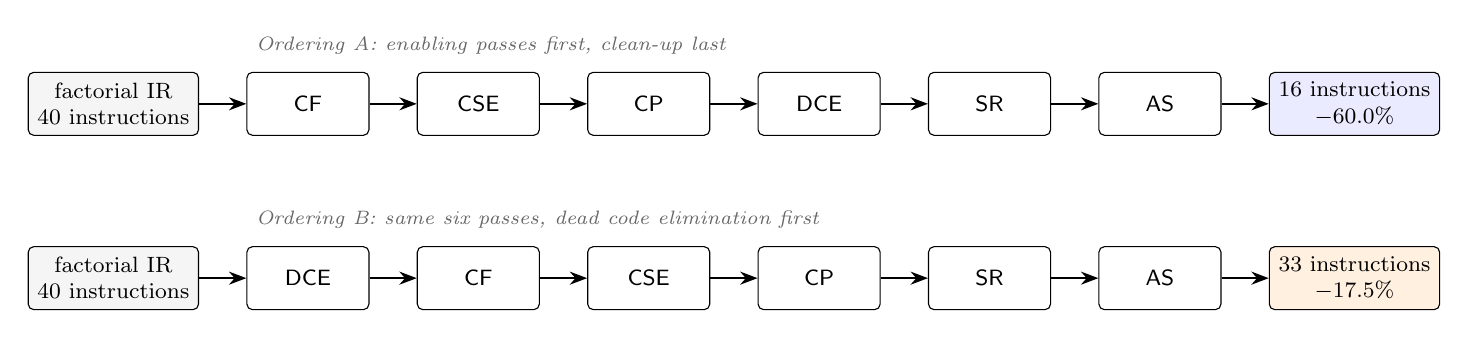
\begin{tikzpicture}[
  node distance=4mm and 6mm,
  box/.style={draw, rounded corners=2pt, minimum width=1.55cm, minimum height=0.8cm, align=center, font=\footnotesize\sffamily, fill=white},
  ir/.style={draw, rounded corners=2pt, minimum width=2.1cm, minimum height=0.8cm, align=center, font=\footnotesize, fill=gray!8},
  res/.style={draw, rounded corners=2pt, minimum width=2.1cm, minimum height=0.8cm, align=center, font=\footnotesize, fill=blue!8},
  arr/.style={-{Stealth[length=2.2mm]}, thick},
  lab/.style={font=\scriptsize\itshape, text=black!60}]
  \node[ir] (in1) {factorial IR\\40 instructions};
  \node[box, right=of in1] (a1) {CF};
  \node[box, right=of a1] (a2) {CSE};
  \node[box, right=of a2] (a3) {CP};
  \node[box, right=of a3] (a4) {DCE};
  \node[box, right=of a4] (a5) {SR};
  \node[box, right=of a5] (a6) {AS};
  \node[res, right=of a6] (o1) {16 instructions\\$-60.0\%$};
  \foreach \s/\t in {in1/a1,a1/a2,a2/a3,a3/a4,a4/a5,a5/a6,a6/o1} \draw[arr] (\s) -- (\t);

  \node[ir, below=14mm of in1] (in2) {factorial IR\\40 instructions};
  \node[box, right=of in2] (b1) {DCE};
  \node[box, right=of b1] (b2) {CF};
  \node[box, right=of b2] (b3) {CSE};
  \node[box, right=of b3] (b4) {CP};
  \node[box, right=of b4] (b5) {SR};
  \node[box, right=of b5] (b6) {AS};
  \node[res, right=of b6, fill=orange!12] (o2) {33 instructions\\$-17.5\%$};
  \foreach \s/\t in {in2/b1,b1/b2,b2/b3,b3/b4,b4/b5,b5/b6,b6/o2} \draw[arr] (\s) -- (\t);

  \node[lab, above=1mm of a1.north west, anchor=south west] {Ordering A: enabling passes first, clean-up last};
  \node[lab, above=1mm of b1.north west, anchor=south west] {Ordering B: same six passes, dead code elimination first};
\end{tikzpicture}}
\caption[The phase-ordering problem in one picture.]{The phase-ordering problem in one picture. The same six passes applied to the same intermediate code of the \code{factorial} benchmark produce a 16-instruction program in one order and a 33-instruction program in another. The only difference is where dead code elimination runs.}
\label{fig:intro-phase-ordering}
\end{figure}

\fig{fig:intro-phase-ordering} shows the effect that motivates the entire project. The unoptimized intermediate code of the \code{factorial} benchmark has 40 instructions. Running the six passes in the order constant folding, common subexpression elimination, copy propagation, dead code elimination, strength reduction, algebraic simplification yields 16 instructions, a reduction of 60\%. Moving dead code elimination to the front and leaving every other pass in the same relative order yields 33 instructions, a reduction of only 17.5\%. No pass was added or removed. The interaction between the passes, and nothing else, accounts for a factor of two in the outcome.

\section{Scope}

The project has a deliberately bounded scope so that the phase-ordering question can be answered completely rather than approximately. The following are within scope and were delivered.

\begin{itemize}
  \item \textbf{Source language.} A subset of C consisting of the \code{int} type, integer literals, arithmetic operators (\code{+}, \code{-}, \code{*}, \code{/}, \code{\%}), comparison operators, logical operators with C short-circuit semantics, unary negation and logical not, global scalar variables with constant initializers, fixed-size one-dimensional arrays, block scoping with shadowing, \code{if}/\code{else}/\code{else if}, \code{while} and \code{for} loops, functions with parameters and return values, a built-in \code{print} statement, and single-line and block comments. Everything is a 32-bit integer; there is no floating point, no pointers, no structures, and no standard library.
  \item \textbf{Compiler front end.} A lexer with line and column tracking, a recursive-descent parser with six levels of operator precedence, an abstract syntax tree of twenty node types, a scope-aware symbol table, and a semantic analyzer that collects every violation in a program and reports them together.
  \item \textbf{Intermediate representation.} A flat three-address code with 35 opcodes, including dedicated opcodes for array and global-variable access so that block-local optimizations cannot miscompile cross-function state.
  \item \textbf{Optimization passes.} Six classical passes: constant folding with constant propagation (\pass{CF}), dead code elimination with unreachable-code removal (\pass{DCE}), common subexpression elimination (\pass{CSE}), copy propagation (\pass{CP}), strength reduction (\pass{SR}), and algebraic simplification (\pass{AS}). Each pass is a pure function from an instruction list to a new instruction list, and each is safe to run in any position of any ordering.
  \item \textbf{Pass manager.} A component that validates and runs an arbitrary ordering, describes it, and enumerates all 720 full permutations plus the baseline.
  \item \textbf{Measurement.} A metric collector that computes static code size, a weighted cycle estimate based on an ARM Cortex-M class cost model, and an instruction-category breakdown; an interpreter that executes the intermediate code and reports dynamic instruction counts, per-opcode frequencies, and program output; and a visualizer that produces seven kinds of publication-quality plots and a geometric-mean summary.
  \item \textbf{Back end.} A RISC-V RV32IM assembly generator producing GNU-syntax, Linux user-mode assembly with a built-in decimal print routine, validated against an in-repository RV32IM simulator so that the assembly is checked to match the interpreter on every benchmark.
  \item \textbf{Benchmarks.} Fifteen kernels: eight adapted from MiBench (bit counting, Collatz iteration, factorial, Fibonacci, greatest common divisor, integer square root, modular exponentiation, and a SHA-style mixing function) and seven adapted from PolyBench/C (one- and two-dimensional Jacobi stencils, GEMM, 2MM, ATAX, BiCG, and GESUMMV).
  \item \textbf{Interactive tool.} A React and TypeScript single-page application served by a FastAPI back end, with five sections: Playground, Optimization Lab, Assembly, Phase-Ordering Explorer, and Reference. A zero-dependency legacy page is also served for environments without a JavaScript build.
  \item \textbf{Quality assurance.} A test suite of 185 automated tests covering every module, including a cross-pass integration test that compiles all fifteen benchmarks under every ordering and asserts output equality with the baseline.
\end{itemize}

The following are explicitly outside the scope of this phase. The compiler does not perform register allocation, instruction scheduling, loop transformations such as unrolling or invariant code motion, inlining, or interprocedural analysis. The optimization passes use local, forward, linear analyses that conservatively reset their state at control-flow boundaries rather than full data-flow analysis over a control-flow graph. The cycle estimate is a static cost model, not a measurement on hardware or in a cycle-accurate simulator. The RISC-V back end uses a simple stack-slot allocation strategy and is intended for faithful, readable lowering rather than peak performance. These exclusions are not weaknesses of the study; they are what make the study tractable. The goal was to characterize the interactions of a small, well-understood set of passes completely, and to build the infrastructure on which more ambitious passes can later be added.

\section{Motivation}

The motivation for this work comes from three directions: education, research, and the practical needs of embedded software.

\textbf{Education.} Compiler design is a core subject in every computer science curriculum, and optimization is usually taught pass by pass: one lecture on constant folding, one on dead code elimination, one on common subexpression elimination. Students learn what each pass does, but they rarely see what the passes do to \emph{each other}. The reason is practical: production compilers are enormous, their pass pipelines are buried under layers of infrastructure, and their intermediate representations are hard to read. Online tools such as Compiler Explorer \cite{godbolt2019} show the final assembly for a given optimization level but do not expose the pipeline that produced it. Recent educational work has begun to address this gap with visualizations of individual optimizations \cite{koitz2025}, but a tool in which a learner can freely rearrange passes and watch the consequences unfold stage by stage did not exist. The team wanted to build one, and to build it on a compiler small enough that a student can read all of its source code in an afternoon.

\textbf{Research.} The phase-ordering problem has a rich literature. Early work used genetic algorithms and other search methods to find good sequences \cite{cooper1999,almagor2004,kulkarni2004}. Kulkarni and colleagues showed that for small sets of passes the space of \emph{distinct outcomes} is far smaller than the space of sequences, because many sequences produce identical code, and that this makes exhaustive enumeration feasible for realistic functions \cite{kulkarni2006,kulkarni2009}. More recent work applies machine learning and reinforcement learning to predict good orderings for LLVM \cite{ashouri2017,hajali2020,jain2022,cummins2023}. Almost all of this work is conducted on production compilers, which means the researcher can never be sure that a measured effect is due to pass interaction rather than to an artefact of the surrounding infrastructure. A small, transparent compiler with a handful of passes offers a complementary view: every ordering can be run, every result can be inspected by hand, and the structural rules that govern the space can be stated exactly. The project is an attempt to produce such a view for six classical passes on embedded-style kernels.

\textbf{Embedded software.} On desktop processors, code size is rarely a concern and the compiler's default pipeline is nearly always good enough. On microcontrollers it is different. A device built around a Cortex-M0 class core may have 32 kilobytes of flash; the difference between a 60\% and a 20\% reduction in code size can decide whether a feature fits at all. Energy consumption is tied directly to the number of cycles executed, so a 20\% reduction in dynamic instructions translates into longer battery life. Studies on embedded targets have found that the standard optimization levels are not always the best choice and that alternative sequences can improve both performance and energy \cite{georgiou2018}. Small manufacturers who build such devices, including the large population of micro, small, and medium enterprises in India, usually cannot afford to tune a compiler for their workload. A framework that quantifies how much ordering matters, and that identifies the structural rules for a good ordering, is a first step towards a tool that could do such tuning automatically. The choice of MiBench, which was designed to represent commercial embedded workloads, and of a RISC-V RV32IM back end, which targets an open instruction set that is increasingly used in low-cost microcontrollers, reflects this motivation.

\textbf{Continuity from Phase I.} The first phase of this project delivered the front end, the intermediate representation, three passes (constant folding, dead code elimination, and common subexpression elimination), a first pass manager, eight MiBench-adapted benchmarks, and a single-file web page for experimentation. The results of that phase, obtained on the \code{factorial} benchmark, showed a 60\% code-size reduction for the best ordering and confirmed that the effect was real and large. Phase II set out to answer the questions that Phase I raised: does the effect hold across a broader and more realistic set of programs, in particular array-based numerical kernels; are there structural rules that explain which orderings are good; how much of the ordering space is redundant; does the improvement in the intermediate code survive lowering to a real instruction set; and can the whole apparatus be made usable by others? Answering those questions required three more passes, seven more benchmarks, a semantic analyzer, arrays, global variables, \code{for} loops, short-circuit evaluation, a RISC-V back end with a simulator to validate it, a redesigned web application, and a substantially larger test suite. This report describes that work and its results.

\textbf{Organization of the report.} Chapter 2 surveys the literature on the phase-ordering problem, on compiler autotuning, on the benchmark suites and evaluation methodology used, and on educational compiler tools. Chapter 3 formulates the problem, states the objectives, and lists the functional and non-functional requirements and the technical specifications. Chapter 4 presents the architecture, high-level and detailed design of every component, describes the fifteen benchmark programs, and lists the tools and technologies used. Chapter 5 reports the experimental environment, the results achieved against each requirement, the empirical findings of the exhaustive phase-ordering study, a comparison with existing work, snapshots of the interactive tool, and the societal impact and Sustainable Development Goals addressed. Chapter 6 concludes and outlines future work. The appendices contain the grammar of the source language, the intermediate-representation opcode reference, a complete compilation trace for one benchmark, and a summary of the test suite.

\chapter{Literature Survey}

The phase-ordering problem has been studied for more than four decades, first as a question of compiler engineering, then as a search problem, and most recently as a machine-learning problem. This chapter reviews the literature that shaped the present work. It is organized in six parts: the classical foundations that define the passes and first recognized their interactions; theoretical results on the nature of the problem; search-based approaches that treat ordering as an optimization problem in its own right; machine-learning approaches that try to predict good orderings; the infrastructure, benchmark suites, and evaluation methodology on which this project rests; and educational tools for making compiler internals visible. The chapter closes with a summary table and a statement of the gap that this project addresses.

\section*{Classical foundations}

Aho, Lam, Sethi, and Ullman \cite{aho2006} provide the standard treatment of the compiler pipeline that this project follows: lexical analysis, syntax analysis by recursive descent, semantic analysis with a scope-aware symbol table, generation of three-address code, and machine-independent optimization. Their chapters on code optimization define the passes implemented in this project, namely constant folding, copy propagation, dead code elimination, common subexpression elimination through available-expression analysis, and strength reduction, and present them as transformations over basic blocks and flow graphs. The book observes that ``the order in which optimizations are applied'' affects results and recommends iterating certain passes to a fixed point, but it does not attempt to characterize the interactions systematically. The three-address code used here, with at most one operator and two operands per instruction and explicit temporaries, follows their presentation closely, as does the treatment of short-circuit boolean expressions through jumping code.

Cooper and Torczon \cite{cooper2011} devote an explicit discussion to the sequencing of optimizations. They note that the compiler writer must decide both which transformations to include and the order in which to apply them, that some transformations create opportunities for others while some destroy them, and that the ideal sequence varies from program to program. They describe the fixed sequence as a compromise and point to their own research on adaptive compilation as an alternative. The book's treatment of local value numbering and of the distinction between local, superlocal, regional, and global optimization scope informed the decision in this project to keep every pass local to a basic block and to reset analysis state at labels and jumps, trading some optimization power for guaranteed safety under arbitrary reordering.

Muchnick \cite{muchnick1997} presents what is probably the best-known prescriptive answer to the phase-ordering question: a diagram that arranges dozens of optimizations into tiers and proposes an order in which they should be run, with constant folding and algebraic simplification early, common subexpression elimination and copy propagation in the middle, and dead code elimination repeatedly as a clean-up step. The order is justified by experience rather than by measurement, and Muchnick explicitly acknowledges that it is a heuristic. The empirical structure uncovered by this project, in which enabling passes must precede clean-up passes and dead code elimination is most effective when it runs last, agrees with Muchnick's recommendation and provides quantitative support for it on a small pass set.

Bacon, Graham, and Sharp \cite{bacon1994} catalogue the program transformations used by optimizing compilers for high-performance computing. Although the catalogue is oriented towards loop and data-layout transformations that are outside the scope of this project, it is valuable for two reasons. It defines each transformation precisely, including the scalar transformations implemented here, and it discusses the legality conditions that a transformation must respect, which guided the conservative handling of arrays and global variables in the passes: because no alias analysis is performed, array loads are never cached across instructions by common subexpression elimination, and array stores and global stores are never removed by dead code elimination.

\section*{The nature of pass interactions}

Whitfield and Soffa \cite{whitfield1997} were among the first to study pass interactions formally. They introduced a specification language, Gospel, in which the preconditions and effects of a code-improving transformation are written down explicitly, and a tool, Genesis, that generates the transformation from the specification. Using the specifications, they derived \emph{enabling} and \emph{disabling} relationships between pairs of transformations: an enabling relationship exists when applying one transformation can create the preconditions for another, and a disabling relationship exists when it can destroy them. Their experiments showed that these relationships are real and measurable, that many pairs interact in both directions, and that the interaction depends on the program. The pairwise interaction matrix produced by this project's visualizer, which compares the mean code size of orderings in which pass A precedes pass B with that of orderings in which B precedes A, is a direct empirical analogue of their enabling and disabling analysis.

Click and Cooper \cite{click1995} approached the interaction problem from a different angle. They showed that, for some pairs of analyses, running them separately in either order is strictly weaker than running a single combined analysis, because each analysis can only exploit the facts that the other has already discovered. Their combined constant propagation and unreachable-code elimination finds constants that no sequence of the two separate passes can find. This result is important for the interpretation of exhaustive phase-ordering studies such as the present one: it establishes that the best sequence of separate passes is not necessarily the best achievable result, and that some phase-ordering problems can only be dissolved by merging passes rather than reordering them. The present project deliberately kept the passes separate in order to study ordering, but this result is a natural direction for future work.

Touati and Barthou \cite{touati2006} examined the decidability of the phase-ordering problem. They modelled optimizations as functions over programs and asked whether an algorithm can decide, for an arbitrary program and performance goal, whether some sequence of optimizations reaches the goal. They proved that the problem is undecidable in the general model where sequences may be arbitrarily long and the performance function is arbitrary, and that it becomes decidable when the sequence length is bounded or when the set of reachable programs is finite. The result justifies the design choice made here: by fixing the set of passes at six and requiring each pass to run exactly once, the ordering space is finite and small, and exhaustive enumeration is not merely feasible but complete.

\section*{Search-based approaches}

Cooper, Schielke, and Subramanian \cite{cooper1999} were the first to treat pass ordering as an explicit optimization problem. Working in a research compiler with ten transformations and targeting code size for embedded systems, they used a genetic algorithm to evolve sequences of twelve passes and compared the result with the compiler's fixed default sequence. The evolved sequences produced substantially smaller code, and, more importantly, the best sequence differed from program to program. Their paper introduced the vocabulary of ``adaptive compilation'' and established code size, rather than execution speed, as a legitimate first-class objective, a framing that this project adopts through its emphasis on static instruction count for embedded targets.

Almagor, Cooper, Grosul, Harvey, Reeves, Subramanian, Torczon, and Waterman \cite{almagor2004} set out to characterize the shape of the search space rather than merely to search it. For a set of small programs they enumerated every sequence of ten passes drawn from five transformations, some $5^{10}$ sequences in all, and studied the distribution of outcomes. They found that the space contains many local minima, that good sequences are nevertheless common, and that simple search strategies such as hill climbing with random restarts find sequences within a few percent of the best in a fraction of the time an exhaustive search would take. The observation that the space, though large, is highly structured is the same observation that emerges from the present project at a smaller scale, where the 720 orderings of six passes collapse into at most 23 distinct outcomes for any single program.

Kulkarni, Hines, Hiser, Whalley, Davidson, and Jones \cite{kulkarni2004} attacked the cost of search. Working in the VISTA interactive compilation framework built on the VPO optimizer, they observed that genetic-algorithm searches over phase sequences wasted most of their time re-evaluating sequences whose outcomes were already known. Two techniques removed the waste: detecting \emph{dormant} phases, which find nothing to do and leave the code unchanged, so that any sequence differing only in dormant phases can be skipped; and hashing the resulting function bodies so that sequences that produce identical code are recognized and evaluated only once. Together these reduced search time by an order of magnitude. Both phenomena are directly visible in this project's data: strength reduction and algebraic simplification are dormant with respect to code size on most benchmarks, and the majority of the 720 orderings produce code identical to some other ordering.

Kulkarni, Whalley, Tyson, and Davidson \cite{kulkarni2006} then asked whether the space could be enumerated exhaustively rather than searched. Their insight was to enumerate not sequences but \emph{distinct function instances}: starting from the unoptimized function, they applied every phase, kept only the results that differed from anything already seen, and repeated until no new instance appeared. Because most sequences produce duplicates, the space of instances is orders of magnitude smaller than the space of sequences. With fifteen reorderable phases they were able to enumerate the complete space of instances for the large majority of functions in their embedded benchmark set, and to determine the truly optimal sequence for each. The exhaustive design of the present project, which enumerates every permutation of a smaller pass set, is a simplified realization of the same idea; the equivalence-class analysis in Chapter 5 is the instance-space view of the same data.

Kulkarni, Whalley, Tyson, and Davidson \cite{kulkarni2009} extended the exhaustive approach to dynamic performance. Because measuring the execution time of every function instance by simulation is expensive, they measured dynamic instruction counts by simulation only for instances with distinct control-flow structure and estimated the rest, achieving near-perfect correlation with full simulation at a small fraction of the cost. They were then able to report, for each function, how far the compiler's default sequence fell short of the optimal one on both size and speed. The present project measures dynamic instruction counts exactly by interpreting every ordering, which is affordable at its scale, and confirms their qualitative finding that size and speed are strongly but not perfectly correlated across orderings.

Triantafyllis, Vachharajani, Vachharajani, and August \cite{triantafyllis2003} proposed Optimization-Space Exploration, in which the compiler compiles each code segment under several optimization configurations and selects the best by a static performance estimate rather than by execution. The configurations are pruned in advance to a small set that covers most of the benefit, and the selection is done at compile time so that the approach fits inside a production compiler. Their use of a static estimator to rank configurations is the same strategy as this project's weighted cycle model; their finding that a small number of well-chosen configurations captures most of the available benefit parallels the observation here that a handful of ordering classes account for all the distinct outcomes.

Hoste and Eeckhout \cite{hoste2008} introduced COLE, Compiler Optimization Level Exploration, which uses a multi-objective evolutionary algorithm to search the space of GCC optimization flags and produces a Pareto front of settings that trade compilation time against execution time. The Pareto-optimal settings outperform the standard levels \code{-O1}, \code{-O2}, and \code{-O3}, and the paper argues that compiler developers should derive their optimization levels by such systematic exploration rather than by hand. The Pareto-front presentation of size against estimated cycles in this project's scatter plots and in the Phase-Ordering Explorer page follows the same multi-objective framing.

Nobre, Martins, and Cardoso \cite{nobre2016} proposed a graph-based approach to pass selection and ordering for LLVM. A directed graph over passes is built from sequences known to perform well, with edge weights reflecting how often one pass follows another; new sequences are then sampled as walks on the graph. The method finds sequences that improve on \code{-O3} for a range of kernels while exploring only a tiny fraction of the space. The idea that good orderings share local structure, that certain passes tend to follow certain others, is borne out by the structural rules found in this project, where every one of the best orderings shares the same relative positions of the four passes that matter.

\section*{Machine-learning approaches}

Agakov, Bonilla, Cavazos, Franke, Fursin, O'Boyle, Thomson, Toussaint, and Williams \cite{agakov2006} were among the first to use machine learning to speed up iterative compilation. Rather than predicting the best sequence directly, they learned a probability distribution over good transformation sequences from a training set of programs and used it to bias the random search on new programs, so that the search concentrated on the promising region of the space. On embedded targets the focused search reached the performance of an unfocused search an order of magnitude faster. The work established the pattern, followed by most later machine-learning approaches, of using static program features to transfer knowledge between programs.

Fursin and colleagues \cite{fursin2011} built this idea into a production compiler with Milepost GCC. The compiler extracts a vector of static features from each function, and a model trained on a corpus of programs predicts which optimization flags to enable. The system was integrated into a mainstream GCC release and demonstrated that learned optimization decisions could be deployed in practice, not only in research prototypes. The features it used, such as counts of instruction kinds, basic blocks, and edges, are the kind of features that this project's metric collector computes as an instruction-category breakdown.

Kulkarni and Cavazos \cite{kulkarnicavazos2012} reformulated phase ordering as a sequential decision problem inside a just-in-time compiler. A neural network, evolved with the NEAT neuroevolution algorithm, examines the current state of the method being compiled and decides which optimization to apply next, one step at a time, until it decides to stop. Because the decision is made from the current code rather than from the original program, the model adapts the sequence as the code changes. Applied to the Jikes research virtual machine, it produced consistent speedups over the default sequence. The stage-by-stage view in this project's Optimization Lab, where the effect of each pass on the current code is displayed before the next pass is chosen, is the interactive, human-driven counterpart of this formulation.

Ashouri, Bignoli, Palermo, Silvano, Kulkarni, and Cavazos \cite{ashouri2017} proposed MiCOMP, which mitigates the phase-ordering problem in LLVM by clustering the optimizer's passes into a small number of sub-sequences and then learning to predict a good ordering of the sub-sequences from program features. The reduction from individual passes to clusters shrinks the search space enough for prediction to be effective, and the predicted orderings outperformed \code{-O3} on a range of benchmarks. The clustering insight, that passes which always travel together can be treated as a unit, is echoed in this project's finding that certain passes never affect the outcome relative to each other and can be collapsed without loss.

Ashouri, Killian, Cavazos, Palermo, and Silvano \cite{ashouri2018} surveyed the field of compiler autotuning with machine learning. The survey classifies the literature by the problem addressed, selection of optimizations versus their ordering; by the learning technique, supervised, unsupervised, or reinforcement learning; by the program representation used as input; and by the target, and identifies open problems including the lack of standard benchmarks and the difficulty of reproducing results across compiler versions. The survey was used in this project as a map of the field and confirmed that small, transparent infrastructures for controlled experimentation are rare.

Haj-Ali, Huang, Moses, Xiang, Stoica, Asanovi\'{c}, and Wawrzynek \cite{hajali2020} introduced AutoPhase, which applies deep reinforcement learning to phase ordering for high-level synthesis, where LLVM passes are applied to a program before it is compiled to hardware and the objective is circuit performance. The agent observes features of the current program and selects the next pass; a random-forest analysis identifies which features matter. AutoPhase reported large improvements over \code{-O3} for the HLS benchmarks studied. The paper is notable for demonstrating that the phase-ordering problem is as relevant to hardware generation as to software, and for showing that reinforcement learning can discover orderings that domain experts would not have chosen.

Jain, Andaluri, VenkataKeerthy, and Upadrasta \cite{jain2022} proposed POSET-RL, which targets the two objectives that matter most for embedded systems, code size and execution time, simultaneously. The method derives a dependence graph from the passes in LLVM's \code{-Oz} size-optimizing pipeline, uses it to constrain the sequences a reinforcement-learning agent may propose, represents programs with learned IR embeddings, and rewards the agent for improving size without degrading time. The reported results improved on \code{-Oz} in code size while maintaining or improving execution time on standard benchmark suites. POSET-RL was the primary inspiration for this project's choice of metrics: static size and a proxy for time are measured for every ordering, and the trade-off between them is the central object of study.

Cummins, Wasti, Guo, Cui, Ansel, Gomez, Jain, Liu, Teytaud, Steiner, Tian, and Leather \cite{cummins2022} released CompilerGym, a set of reinforcement-learning environments for compiler optimization problems built in the style of OpenAI Gym. The LLVM environment exposes phase ordering as an environment whose actions are passes and whose rewards are changes in code size or runtime, together with standard benchmark datasets and baselines. The project made phase-ordering research reproducible and accessible to machine-learning researchers without compiler expertise. This project's web API, which exposes compile, optimize, step, and benchmark endpoints over HTTP, is a much smaller but philosophically similar attempt to make a phase-ordering environment available to others.

VenkataKeerthy, Aggarwal, Jain, Desarkar, Upadrasta, and Srikant \cite{venkatakeerthy2020} developed IR2Vec, a method for embedding LLVM intermediate representation into continuous vectors that capture the semantics of the code. The embeddings are computed from the IR itself, without executing the program, and are used as input features by POSET-RL and other learning-based phase-ordering systems. The work illustrates how much effort the machine-learning approaches must invest in representing programs before any learning can begin, and by contrast how simple the representation problem becomes in an infrastructure such as this project's, where the IR has 35 opcodes and the entire program is a short list of instructions.

Cummins, Seeker, Grubisic, Elhoushi, Liang, Roziere, Gehring, Gloeckle, Hazelwood, Synnaeve, and Leather \cite{cummins2023} trained a large language model to optimize LLVM assembly. Given an unoptimized function, the model emits the list of passes that should be applied to minimize code size, and as an auxiliary task it predicts the resulting instruction count and the optimized code itself. The model improved on \code{-Oz} by a few percent over a large test set without executing any compilation during inference. The work represents the current frontier of learning-based phase ordering and highlights that even the most capable models are being evaluated against exactly the metric this project uses, static instruction count.

Han and Kim \cite{han2024} observed that many passes in a sequence are dormant, changing nothing, and that a search algorithm which can predict dormancy can effectively explore an exponentially larger space of sequences for the same cost, since every dormant pass can be inserted or removed without evaluation. They learned to predict dormancy from program features and integrated the predictor into a phase-ordering search. This is a modern, learned version of the dormant-phase detection of Kulkarni et al.\ \cite{kulkarni2004}, and it is precisely the phenomenon that produces the large equivalence classes in this project's results.

Liu and colleagues \cite{liu2024} proposed to model the dependence between passes explicitly and to use the dependence model to prune the ordering search, so that passes known to be independent are not permuted and passes known to depend on one another are kept in the beneficial order. Their approach reduced search cost while preserving optimization quality. Chen, Chen, Yao, Yu, Xu, and Ma \cite{chen2025} identified short chains of passes that reliably boost the effectiveness of the passes that follow them, and built phase-ordering sequences around these booster chains. Both papers, published after this project began, articulate the same structural view that this project's results support empirically: the ordering space is governed by a small number of dependence relationships among a subset of the passes, and once those are respected the remaining freedom is inconsequential.

\section*{Infrastructure, targets, and cost models}

Lattner and Adve \cite{lattner2004} described the LLVM compiler infrastructure, whose modular pass framework and typed, static-single-assignment intermediate representation have made it the platform for almost all recent phase-ordering research. LLVM's pass manager accepts an explicit list of passes and runs them in the given order, which is what makes the phase-ordering experiments of \cite{ashouri2017,hajali2020,jain2022,cummins2023} possible. The pass manager in this project is modelled on the same idea at a much smaller scale: a registry of named passes, a validated ordered list, and a loop that threads the IR through each pass in turn. LLVM was not used directly because its scale, with over a hundred passes and an IR that a student cannot read at a glance, defeats the purpose of a transparent teaching and research tool.

Waterman and Asanovi\'{c} \cite{waterman2019} specify the RISC-V unprivileged instruction set architecture. RISC-V is an open, royalty-free ISA whose base integer instruction set, RV32I, together with the multiply and divide extension, M, defines the RV32IM target chosen for this project's back end. The specification's small, regular instruction set makes it possible to write a correct code generator and a validating simulator in a few hundred lines each, and its rapidly growing adoption in low-cost microcontrollers makes it a realistic embedded target. The specification also documents the behaviour of division by zero, which the back end must guard explicitly to match the interpreter's semantics.

The ARM Cortex-M3 Technical Reference Manual \cite{arm2010} provided the instruction timing information from which this project's cost model was derived. On Cortex-M class cores, most arithmetic, logical, and comparison instructions execute in a single cycle; multiplication takes one to several cycles depending on the core; hardware division takes between two and twelve cycles depending on the operands; taken branches incur a pipeline refill penalty of several cycles; and loads and stores take two cycles. The cost model assigns weights in this spirit, one cycle for simple operations, three for multiplication, twelve for division and modulo, two for branches and memory accesses, and larger fixed costs for calls, returns, and output. The model is an estimate, not a measurement, and Chapter 5 discusses its limitations.

Georgiou, Blackmore, Xavier-de-Souza, and Eder \cite{georgiou2018} studied the standard optimization levels of GCC and LLVM on Cortex-M embedded targets from the point of view of both performance and energy consumption. They found that the highest optimization level is frequently not the best choice on these targets, that lower levels sometimes produce faster and more energy-efficient code, and that the reasons lie in pass interactions and target-specific effects that the default pipelines do not account for. They proposed a lightweight approach that exploits the existing levels rather than searching the full flag space. Their work supports the premise of this project that the phase-ordering problem is of practical importance on embedded targets and that the default pipeline is not the last word.

\section*{Benchmark suites and evaluation methodology}

Guthaus, Ringenberg, Ernst, Austin, Mudge, and Brown \cite{guthaus2001} introduced MiBench, a free benchmark suite designed to be representative of commercial embedded workloads. The suite is organized into six categories, automotive and industrial control, consumer devices, office automation, networking, security, and telecommunications, and its programs are small enough to run on a simulator yet realistic enough that their characteristics differ measurably from the desktop-oriented SPEC suites. Eight of this project's fifteen benchmarks are adapted from MiBench kernels: bit counting from the automotive category, integer square root and basic arithmetic kernels from basicmath, and modular exponentiation and hash mixing from the security category. The adaptations preserve the control structure and arithmetic character of the originals while restricting them to the integer subset of C that the compiler supports.

Pouchet and Yuki \cite{pouchet2016} maintain PolyBench/C, a collection of numerical kernels from linear algebra, stencil computations, data mining, and medley categories, written in a restricted style that makes them amenable to polyhedral analysis. Each kernel is a small set of nested loops over arrays with affine index expressions. Seven of this project's benchmarks are adapted from PolyBench: the one- and two-dimensional Jacobi stencils, general matrix multiplication (GEMM), two chained matrix multiplications (2MM), matrix-transpose-vector product (ATAX), the BiCG sub-kernel, and the scalar-vector-matrix product GESUMMV. These kernels were added in Phase II to test whether the phase-ordering effects observed on scalar MiBench kernels carry over to array-based numerical code with repeated index arithmetic, which they do.

Fleming and Wallace \cite{fleming1986} showed, in a widely cited note, that the arithmetic mean is the wrong way to summarize normalized benchmark results, because the ranking it produces depends on which system is chosen as the normalization base. The geometric mean is the only mean that is consistent under normalization, and it is therefore the correct aggregate for ratios such as ``optimized size divided by baseline size''. All cross-program summaries in this project are geometric means of per-program ratios, computed as the exponential of the mean logarithm, and every result table that reports an average across programs follows this rule.

\section*{Educational compiler tools}

Godbolt \cite{godbolt2019} described Compiler Explorer, the widely used web tool that shows, for a program typed into the browser, the assembly produced by dozens of compilers at any optimization level, with source lines colour-linked to assembly lines. The article walks through the optimizations a modern compiler performs and shows how the tool reveals them. Compiler Explorer inspired the side-by-side, hover-linked presentation of intermediate code and RISC-V assembly in this project's Assembly page. It differs from this project in that it treats the compiler as a black box with a fixed pipeline; the user can choose \code{-O2} but cannot reorder the passes within it or see the intermediate stages.

Koitz-Hristov, Mandl, and Wotawa \cite{koitz2025} presented VisOpt, an educational tool that visualizes compiler optimizations for computer science students, showing the effect of individual transformations on program representations to support teaching of compiler construction. Their evaluation in a classroom setting found that visualization improved students' understanding of what the optimizations do. This project shares VisOpt's goal and extends it in one specific direction: it visualizes not only individual optimizations but their interaction, by letting the learner change the order and observe the consequence at each stage.

Nystrom \cite{nystrom2021} and Sandler \cite{sandler2024} are recent book-length tutorials on building interpreters and C compilers from scratch. Both emphasize hand-written lexers and recursive-descent parsers, incremental development with a test suite, and a three-address or similar linear intermediate form, and Sandler's book in particular covers the implementation of constant folding, copy propagation, unreachable-code elimination, and dead-store elimination as separate passes over a three-address code, together with a discussion of the order in which to run them. These works guided the engineering style of this project's front end and confirmed that a compiler of this scope can be implemented, tested, and understood by a small student team.

\section*{Summary and research gap}

Table~\ref{tab:lit-summary} summarizes the surveyed work by approach, the compiler on which it was carried out, the scale of the pass set, and the objective measured.

\begin{table}[!tbp]
\centering\footnotesize
\caption{Summary of the surveyed work on phase ordering and compiler autotuning}
\label{tab:lit-summary}
\begin{tabular}{L{3.1cm} L{2.7cm} L{2.3cm} L{1.7cm} L{2.7cm}}
\toprule
\textbf{Work} & \textbf{Approach} & \textbf{Compiler} & \textbf{Passes} & \textbf{Objective}\\
\midrule
Whitfield \& Soffa \cite{whitfield1997} & Formal enabling / disabling relations & Genesis & few & interaction analysis\\
Cooper et al.\ \cite{cooper1999} & Genetic algorithm & research (MSCP) & 10 & code size\\
Almagor et al.\ \cite{almagor2004} & Exhaustive sub-space, hill climbing & research & 5 (len.\ 10) & speed, size\\
Kulkarni et al.\ \cite{kulkarni2004} & GA with dormancy and hashing & VPO / VISTA & 15 & size, speed\\
Kulkarni et al.\ \cite{kulkarni2006,kulkarni2009} & Exhaustive instance enumeration & VPO & 15 & size, dyn.\ count\\
Triantafyllis et al.\ \cite{triantafyllis2003} & Configuration exploration, static estimator & Itanium research & configurations & speed\\
Hoste \& Eeckhout \cite{hoste2008} & Multi-objective evolutionary & GCC & flags & Pareto speed / compile time\\
Agakov et al.\ \cite{agakov2006}, Fursin et al.\ \cite{fursin2011} & ML-focused search, learned flag prediction & GCC & flags & speed\\
Kulkarni \& Cavazos \cite{kulkarnicavazos2012} & Neuroevolution, per-step decision & Jikes RVM & tens & speed\\
Ashouri et al.\ \cite{ashouri2017} & Clustered sub-sequences, supervised ML & LLVM & $\sim$100 & speed\\
Haj-Ali et al.\ \cite{hajali2020} & Deep RL & LLVM / HLS & 45 & circuit perf.\\
Jain et al.\ \cite{jain2022} & Deep RL with dependence graph & LLVM & $\sim$30 & size and time\\
Cummins et al.\ \cite{cummins2022,cummins2023} & RL environments; LLM pass prediction & LLVM & $\sim$120 & size\\
Han \& Kim \cite{han2024}, Liu et al.\ \cite{liu2024}, Chen et al.\ \cite{chen2025} & Dormancy, dependence, booster chains & LLVM & $\sim$100 & size, speed\\
Georgiou et al.\ \cite{georgiou2018} & Standard-level analysis on Cortex-M & GCC, LLVM & levels & speed, energy\\
Godbolt \cite{godbolt2019}, Koitz-Hristov et al.\ \cite{koitz2025} & Visualization for learners & GCC, LLVM, others & fixed & education\\
\textbf{This project} & \textbf{Exhaustive 721-ordering enumeration, equivalence-class analysis, interactive tool} & \textbf{custom, transparent} & \textbf{6} & \textbf{size, est.\ cycles, dyn.\ count}\\
\bottomrule
\end{tabular}
\end{table}

Three observations follow from the survey. First, almost all quantitative phase-ordering research has been conducted on production compilers, chiefly LLVM, GCC, and VPO. This has the advantage of realism but the disadvantage of opacity: with a hundred passes and a complex IR, the researcher measures the aggregate effect of ordering but cannot easily attribute it to specific pairwise interactions, and a student cannot follow what happened. Second, the search-based and learning-based methods are motivated by the impossibility of exhaustive enumeration at production scale, and they therefore report how much better than the default a found sequence is, but rarely how far from the true optimum it remains; only the exhaustive studies of Kulkarni and colleagues can answer that question, and they did so for a fixed set of fifteen phases in a single research compiler. Third, educational tools show the effect of a fixed pipeline or of single optimizations, but none allows a learner to reorder passes and observe the consequences stage by stage.

The gap that this project addresses lies at the intersection of these three observations. It builds a compiler infrastructure small enough that every pass and every intermediate result can be read, in which the ordering space is small enough to enumerate completely, so that the true optimum and the structure of the space are known exactly rather than estimated; it evaluates on kernels adapted from the embedded and numerical benchmark suites used by the wider community, with the metrics, size, time proxy, and dynamic count, that the community uses; it lowers the results to a real instruction set to check that improvements in the IR survive code generation; and it wraps the whole in an interactive tool that makes the phase-ordering problem visible to learners. None of the surveyed works combines these properties.

\chapter{Problem Formulation}

\section{Problem Description}

An optimizing compiler applies a sequence of transformation passes to an intermediate representation of a program. Let $P$ denote a program in intermediate form and let $\Pi = \{\pi_1, \pi_2, \ldots, \pi_n\}$ be a set of $n$ optimization passes, each a function that maps a program to a semantically equivalent program. A \emph{phase ordering} is a permutation $\sigma$ of $\{1, \ldots, n\}$, and applying it to $P$ produces
\[
  P_\sigma = \pi_{\sigma(n)}\bigl(\pi_{\sigma(n-1)}(\cdots \pi_{\sigma(1)}(P)\cdots)\bigr).
\]
Let $m$ be a metric on programs, such as the number of instructions or an estimate of the cycles needed to execute them. The phase-ordering problem asks for the permutation $\sigma^\ast$ that minimizes $m(P_\sigma)$ for a given $P$, or for a fixed $\sigma$ that performs well over a population of programs.

The problem is hard for reasons that are structural rather than incidental. The number of permutations is $n!$, so the space grows faster than any polynomial in $n$. The passes are not commutative: $\pi_i(\pi_j(P))$ and $\pi_j(\pi_i(P))$ are in general different programs, because a transformation changes the very patterns that the other transformation looks for. Nor are the passes idempotent in combination: even though a single pass may reach a fixed point on its own, running it again after another pass has changed the program can find new work. The optimal permutation depends on $P$, so no fixed $\sigma$ is best for every program. And the dependence of $m(P_\sigma)$ on $\sigma$ is not smooth in any useful sense; two permutations that differ in one adjacent swap can produce very different programs, while two permutations that differ in many positions can produce identical ones.

In practice, three further complications appear. First, the metric is not unique. Code size matters for flash-constrained embedded devices, execution time matters for everything else, and the two do not always move together; a transformation that shortens the code may lengthen the critical loop, and one that speeds up the loop may duplicate code. The problem is therefore multi-objective, and its solution is a Pareto front rather than a single point. Second, correctness must be preserved under every ordering. A pass that is correct in the position its author intended may be incorrect in another position if it relies on an invariant that an earlier pass established; a system that permits arbitrary reordering must ensure that every pass is correct on any valid input. Third, the results of an ordering study are only meaningful if the passes are studied on programs that resemble real workloads, which requires a benchmark suite and a principled way of aggregating results across it.

Production compilers sidestep the problem with a fixed pipeline that has been tuned over many years. This is a sound engineering decision, but it leaves several questions unanswered for anyone who is not a maintainer of that compiler. How much does the ordering actually matter for a given set of passes and a given class of programs? Which pairs of passes interact, in which direction, and how strongly? How much of the ordering space is redundant, in the sense that different orderings produce the same result? Is there a simple structural rule that characterizes the good orderings? Does an improvement measured on the intermediate representation survive translation to a real instruction set? These questions can be answered exactly only by enumerating the space, which is impossible at production scale and has been done in the literature only once, for one research compiler.

The project therefore studies a bounded instance of the problem: six classical scalar optimizations on a subset of C, evaluated on fifteen kernels adapted from embedded and numerical benchmark suites, with the ordering space enumerated in full. The bounded instance is chosen so that the answers are complete and inspectable, and so that the infrastructure that produces them is small enough to serve as a teaching tool.

\section{Problem Statement}

Existing compiler infrastructures apply optimization passes in a fixed, hand-tuned order, and the size and complexity of those infrastructures make it impractical to isolate, reorder, and measure individual passes or to enumerate the space of orderings. As a result, the quantitative effect of phase ordering on code size and execution cost is known only approximately, the structure of the ordering space is understood only through sampled search, and students and engineers have no transparent environment in which to observe how optimization passes interact.

The project addresses this by designing and implementing a modular compiler for a subset of C in which every optimization pass is an independent, reorderable, and individually correct transformation on a three-address-code intermediate representation; by building a pass manager that can run any ordering and enumerate all of them; by measuring static code size, an estimated cycle cost, and the dynamic instruction count of every ordering on a suite of fifteen MiBench- and PolyBench-derived kernels; by validating correctness of every optimized program against the unoptimized baseline through execution; by lowering the optimized code to RISC-V RV32IM assembly and validating that as well; and by presenting the entire pipeline, the orderings, and the resulting trade-offs in an interactive web application.

\section{Objectives}

\begin{enumerate}
  \item To design and implement a complete compiler front end for a subset of C, comprising a lexer, a recursive-descent parser producing an abstract syntax tree, a scope-aware symbol table, and a semantic analyzer that reports all violations in a single pass.
  \item To define a three-address-code intermediate representation with explicit support for functions, control flow, fixed-size arrays, and global variables, together with an IR generator that translates the syntax tree into it, and an interpreter that executes it.
  \item To implement six classical optimizations, constant folding, dead code elimination, common subexpression elimination, copy propagation, strength reduction, and algebraic simplification, as independent passes that are correct in any position of any ordering.
  \item To build a configurable pass manager that runs an arbitrary ordering and enumerates all $6! = 720$ full permutations together with the unoptimized baseline.
  \item To adapt fifteen benchmark kernels from the MiBench embedded suite and the PolyBench/C numerical suite into the supported subset of C.
  \item To measure, for every program and every ordering, the static code size, an estimated cycle count based on an embedded-processor cost model, and the dynamic instruction count, and to verify that the program output is unchanged.
  \item To analyze the results: identify the best and worst orderings per program and overall using geometric-mean aggregation, quantify pairwise pass interactions, determine the equivalence classes of orderings that produce identical outcomes, and characterize the structural rules that distinguish good orderings from bad ones.
  \item To implement a RISC-V RV32IM assembly back end and an accompanying simulator, and to verify that every benchmark produces the same output when lowered to assembly as when interpreted.
  \item To develop an interactive web application that exposes every stage of the compiler, allows passes to be reordered by drag and drop, steps through the pipeline with a diff at each stage, displays the generated assembly, and runs the exhaustive ordering exploration in the browser.
  \item To achieve comprehensive automated test coverage of every component, including an end-to-end test that compiles all benchmarks under all orderings.
\end{enumerate}

\section{Functional Requirements}

\begin{itemize}
  \item \textbf{FR-1 Lexical analysis.} The system shall convert source text in the supported C subset into a token stream with line and column information, recognizing keywords, identifiers, integer literals, all supported operators and delimiters, and skipping single-line and block comments. Malformed input shall produce an error that names the offending location.
  \item \textbf{FR-2 Syntax analysis.} The system shall parse the token stream into an abstract syntax tree according to the grammar in Appendix~A, respecting the six levels of operator precedence, and shall report the first syntax error with its location and the token that was found.
  \item \textbf{FR-3 Semantic analysis.} The system shall check that every variable is declared before use, that no name is declared twice in one scope, that called functions exist and are called with the correct number of arguments, that no function is defined twice, that arrays are indexed and scalars are not, that a \code{main} function exists, and that global initializers are compile-time constants. All violations in a program shall be collected and reported together.
  \item \textbf{FR-4 Intermediate code generation.} The system shall translate a semantically valid syntax tree into three-address code, using explicit temporaries and labels, dedicated opcodes for array and global access, and jumping code for short-circuit logical operators.
  \item \textbf{FR-5 Interpretation.} The system shall execute the intermediate code directly, producing the program's printed output and return value, the total number of instructions executed, and the number of executions of each opcode, with a step limit that prevents non-terminating programs from hanging the system.
  \item \textbf{FR-6 Optimization passes.} The system shall provide the six passes \pass{CF}, \pass{DCE}, \pass{CSE}, \pass{CP}, \pass{SR}, and \pass{AS}, each as a function from an instruction list to a new instruction list, each preserving program semantics on any valid input regardless of what passes ran before it.
  \item \textbf{FR-7 Pass ordering.} The system shall accept any ordered list of pass names, validate it, apply the passes in the given order, and describe the ordering in human-readable form. It shall enumerate all full permutations of the six passes together with the empty ordering.
  \item \textbf{FR-8 Metric collection.} The system shall compute, for any instruction list, the static code size excluding labels and structural markers, an estimated cycle count from a documented per-opcode cost table, and a breakdown of instructions by category.
  \item \textbf{FR-9 Exhaustive benchmarking.} The system shall compile a program under every ordering, execute each result, record all three metrics, verify that the output matches the baseline, and report the results as a table, as per-program plots, and as a geometric-mean summary across programs.
  \item \textbf{FR-10 RISC-V code generation.} The system shall translate intermediate code, optimized or not, into RV32IM assembly in GNU syntax for Linux user mode, including a runtime routine that prints integers, and shall provide a mapping from each intermediate instruction to the assembly lines it produced.
  \item \textbf{FR-11 Interactive web application.} The system shall serve a browser application through which a user can edit or load a program, compile it and inspect tokens, syntax tree, symbols, and intermediate code with error locations highlighted in the editor; arrange the passes in any order and run them, viewing the intermediate code after each stage with a diff and metric deltas; view the assembly side by side with the intermediate code; run all orderings and explore the results in an interactive size-versus-cycles plot; and consult a reference page describing the passes, cost model, and language.
  \item \textbf{FR-12 Command-line interface.} The system shall provide a command-line tool that compiles a file, optionally with a given pass ordering, prints tokens, syntax tree, intermediate code, and metrics on request, emits assembly, and runs the benchmark on one program or on all benchmark programs.
\end{itemize}

\section{Non-Functional Requirements}

\begin{itemize}
  \item \textbf{NFR-1 Correctness.} Every optimized program, under every ordering, shall produce output identical to the unoptimized program. Every program lowered to RISC-V assembly shall produce output identical to the interpreter. These properties shall be enforced by automated tests.
  \item \textbf{NFR-2 Determinism and reproducibility.} Given the same source and the same ordering, the system shall produce byte-identical intermediate code, assembly, and metrics on every run and on every machine.
  \item \textbf{NFR-3 Performance.} The exhaustive 721-ordering benchmark of a single program, including interpretation of every result, shall complete in under ten seconds on a contemporary laptop, so that it can be run interactively from the web application. The full benchmark of all fifteen programs shall complete in under one minute.
  \item \textbf{NFR-4 Transparency and readability.} Each compiler module shall be a single, self-contained source file of a few hundred lines with a module-level description of its algorithm, so that a student can read and understand any component in isolation.
  \item \textbf{NFR-5 Portability and ease of installation.} The compiler and web server shall run on any platform with Python 3.10 or later and shall require no compiled extensions, no database, and no external services. The web front end shall be pre-built and committed so that a fresh clone runs with a single Python command and no JavaScript toolchain. The application shall work fully offline with no content-delivery-network dependencies.
  \item \textbf{NFR-6 Usability.} The web application shall be operable with the mouse or with the keyboard alone, shall report compiler errors with the phase, message, and source location, and shall respond to compile and optimize requests within one second for programs of benchmark size.
  \item \textbf{NFR-7 Maintainability and test coverage.} Every module shall have automated tests; the test suite shall run in under one minute and shall be executed before every change is merged. The code shall follow a consistent style with type annotations throughout.
  \item \textbf{NFR-8 Extensibility.} Adding a new optimization pass shall require only a new module exporting one function and one line in the pass registry; the pass manager, benchmark, web API, and user interface shall pick it up without further change.
\end{itemize}

\section{Technical Specifications}

\textbf{Source language}
\begin{itemize}
  \item A subset of C: \code{int} type only; integer literals; arithmetic, comparison, and logical operators; unary minus and logical not; assignment as statement and expression.
  \item Declarations: local and global scalars with optional initializers, fixed-size one-dimensional local arrays with zero initialization, function definitions with integer parameters.
  \item Statements: expression, block, \code{if}/\code{else}/\code{else if}, \code{while}, \code{for} with optional clauses, \code{return}, and built-in \code{print}.
  \item Semantics: 32-bit two's-complement integers in the back end and Python integers in the interpreter; division and modulo by zero yield zero in both; short-circuit evaluation of \code{\&\&} and \code{||}.
\end{itemize}

\textbf{Compiler implementation}
\begin{itemize}
  \item Language: Python 3.12 with type annotations and dataclasses; no third-party dependencies in the compiler core.
  \item Intermediate representation: linear three-address code, 35 opcodes, immutable instruction records, per-instruction def/use analysis.
  \item Optimization passes: six pure functions; local forward analyses with state reset at control-flow boundaries; fixed-point iteration within constant folding and dead code elimination.
  \item Back end: RISC-V RV32IM, GNU assembler syntax, Linux user-mode system calls for output and exit, stack-slot allocation with 16-byte-aligned frames.
\end{itemize}

\textbf{Measurement and visualization}
\begin{itemize}
  \item Metrics: static instruction count; weighted cycle estimate (ARM Cortex-M class weights: 1 cycle for simple ALU and copy operations, 3 for multiplication, 12 for division and modulo, 2 for branches and memory access, 5 for call, 3 for return, 10 for output); dynamic instruction count and per-opcode frequency from the interpreter.
  \item Aggregation: per-program normalization to the baseline; geometric mean across programs.
  \item Plots: matplotlib 3.11 and NumPy 1.26; seven plot types at 150 dpi.
\end{itemize}

\textbf{Web application}
\begin{itemize}
  \item Back end: FastAPI 0.141 on Uvicorn 0.52 with Pydantic 2 request and response models; seven JSON endpoints; same-origin static file serving.
  \item Front end: React 19 with TypeScript 6, built with Vite 8; CodeMirror 6 editor with a C language mode and a lint gutter; Chart.js 4 for interactive plots; bundled Inter, JetBrains Mono, and Space Grotesk fonts.
  \item Legacy front end: a zero-dependency single-file HTML, CSS, and JavaScript page served at a secondary route.
\end{itemize}

\textbf{Testing and tooling}
\begin{itemize}
  \item pytest 9 with 185 test cases across three test modules; an in-repository RV32IM simulator used as a test oracle for the back end.
  \item Git version control with 54 commits by the team members over February to August 2026; GitHub hosting.
  \item Development on Linux (Linux Mint 22.2, kernel 6.17) and Windows; Visual Studio Code; Node.js 20 or later for front-end development only.
\end{itemize}

\textbf{Hardware requirements}
\begin{itemize}
  \item Any 64-bit machine with 4 GB of RAM is sufficient to run the compiler, the tests, and the web application. The reference machine used for all reported timings is an AMD Ryzen 7 7435HS laptop with 8 cores, 16 threads, and 24 GB of RAM.
  \item Optional: a RISC-V cross toolchain (\code{riscv64-linux-gnu-gcc}) and \code{qemu-riscv32} to run the generated assembly on emulated hardware; not required, since the bundled simulator validates the assembly.
\end{itemize}

\chapter{Project Design and Implementation}

\section{Proposed Project Architecture}

The system is organized as a layered pipeline in which each layer consumes a well-defined data structure from the layer above it and produces one for the layer below. The layering is the direct consequence of the requirement that every optimization pass be independent and reorderable: if a pass could reach into the parser, or the code generator could depend on which passes had run, ordering experiments would be confounded by hidden coupling. Every boundary in \fig{fig:architecture} is therefore a plain Python data structure, a list of tokens, a syntax tree, a list of instructions, or a metrics record, and no layer holds a reference to any other layer's internal state.

\begin{figure}[!htb]
\centering
\resizebox{\textwidth}{!}{%
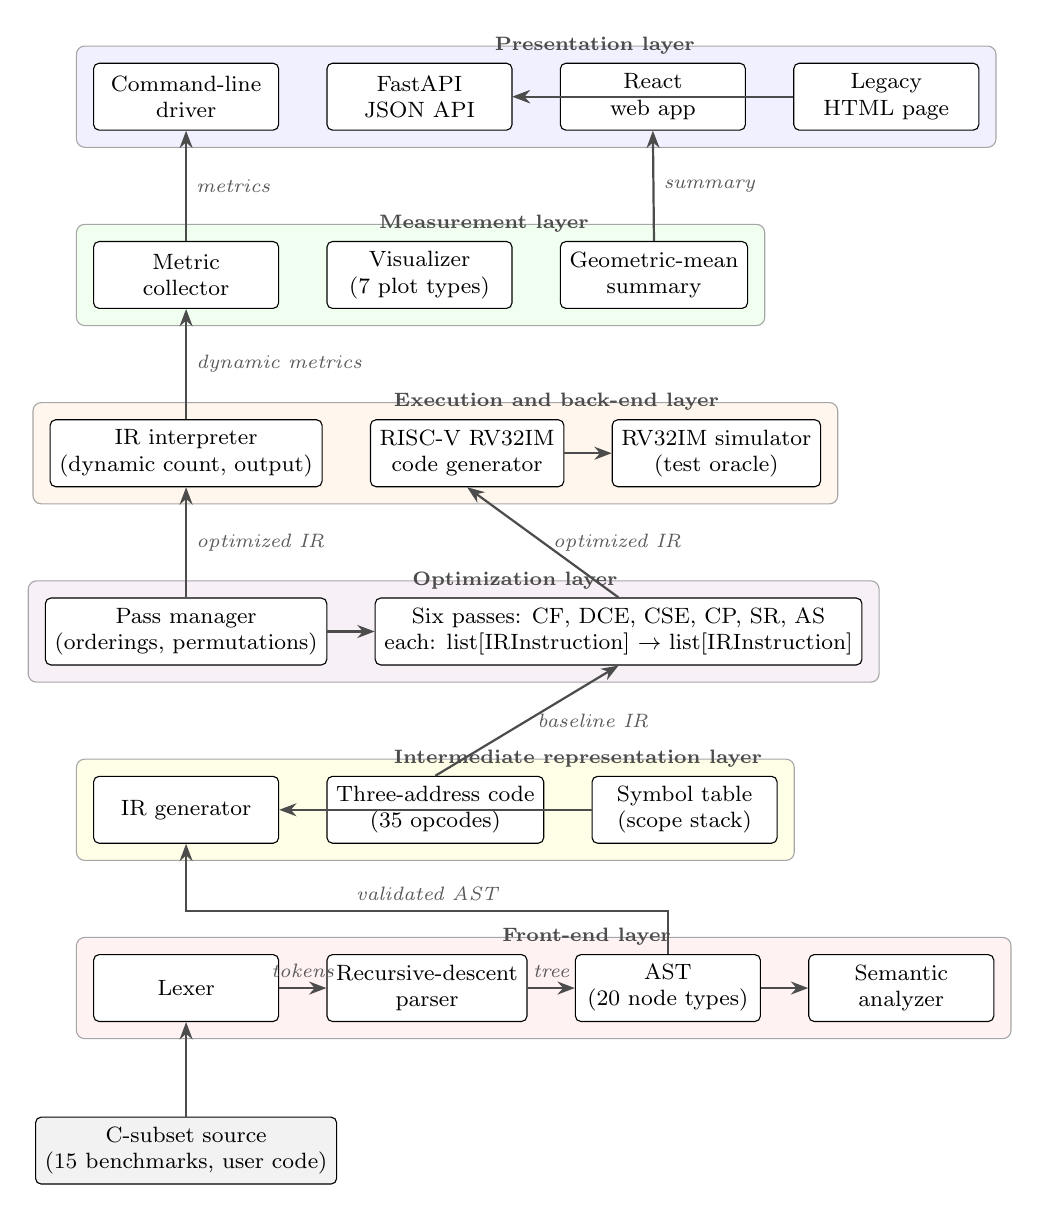
\begin{tikzpicture}[
  font=\footnotesize,
  layer/.style={draw=black!35, rounded corners=3pt, inner sep=6pt, fill=#1},
  comp/.style={draw, rounded corners=2pt, fill=white, minimum height=0.85cm, minimum width=2.35cm, align=center, font=\footnotesize},
  data/.style={font=\scriptsize\itshape, text=black!65},
  arr/.style={-{Stealth[length=2.2mm]}, thick, black!70},
  lbl/.style={font=\scriptsize\bfseries, text=black!70, anchor=west}]

% Presentation layer
\node[comp] (cli) at (0,0) {Command-line\\driver};
\node[comp, right=6mm of cli] (api) {FastAPI\\JSON API};
\node[comp, right=6mm of api] (react) {React\\web app};
\node[comp, right=6mm of react] (legacy) {Legacy\\HTML page};
\begin{scope}[on background layer]
\node[layer=blue!6, fit=(cli)(legacy), label={[lbl]above left:Presentation layer}] (L6) {};
\end{scope}
\draw[arr] (react) -- (api);
\draw[arr] (legacy) -- (api);

% Measurement layer
\node[comp, below=14mm of cli] (metrics) {Metric\\collector};
\node[comp, right=6mm of metrics] (viz) {Visualizer\\(7 plot types)};
\node[comp, right=6mm of viz] (geo) {Geometric-mean\\summary};
\begin{scope}[on background layer]
\node[layer=green!6, fit=(metrics)(geo), label={[lbl]above left:Measurement layer}] (L5) {};
\end{scope}

% Execution / backend layer
\node[comp, below=14mm of metrics] (interp) {IR interpreter\\(dynamic count, output)};
\node[comp, right=6mm of interp] (codegen) {RISC-V RV32IM\\code generator};
\node[comp, right=6mm of codegen] (sim) {RV32IM simulator\\(test oracle)};
\begin{scope}[on background layer]
\node[layer=orange!7, fit=(interp)(sim), label={[lbl]above left:Execution and back-end layer}] (L4) {};
\end{scope}
\draw[arr] (codegen) -- (sim);

% Optimization layer
\node[comp, below=14mm of interp] (pm) {Pass manager\\(orderings, permutations)};
\node[comp, right=6mm of pm, minimum width=5.1cm] (passes) {Six passes: CF, DCE, CSE, CP, SR, AS\\each: list[IRInstruction] $\to$ list[IRInstruction]};
\begin{scope}[on background layer]
\node[layer=violet!6, fit=(pm)(passes), label={[lbl]above left:Optimization layer}] (L3) {};
\end{scope}
\draw[arr] (pm) -- (passes);

% Middle layer
\node[comp, below=14mm of pm] (irgen) {IR generator};
\node[comp, right=6mm of irgen] (ir) {Three-address code\\(35 opcodes)};
\node[comp, right=6mm of ir] (symtab) {Symbol table\\(scope stack)};
\begin{scope}[on background layer]
\node[layer=yellow!10, fit=(irgen)(symtab), label={[lbl]above left:Intermediate representation layer}] (L2) {};
\end{scope}
\draw[arr] (symtab) -- (irgen);

% Front end
\node[comp, below=14mm of irgen] (lexer) {Lexer};
\node[comp, right=6mm of lexer] (parser) {Recursive-descent\\parser};
\node[comp, right=6mm of parser] (ast) {AST\\(20 node types)};
\node[comp, right=6mm of ast] (sema) {Semantic\\analyzer};
\begin{scope}[on background layer]
\node[layer=red!5, fit=(lexer)(sema), label={[lbl]above left:Front-end layer}] (L1) {};
\end{scope}
\draw[arr] (lexer) -- node[data, above]{tokens} (parser);
\draw[arr] (parser) -- node[data, above]{tree} (ast);
\draw[arr] (ast) -- (sema);

% Source
\node[comp, below=12mm of lexer, fill=gray!10] (src) {C-subset source\\(15 benchmarks, user code)};
\draw[arr] (src) -- (lexer);

% Vertical flows between layers
\draw[arr] (ast.north) -- ++(0,0.55) -| node[data, pos=0.25, above]{validated AST} (irgen.south);
\draw[arr] (ir.north) -- node[data, right]{baseline IR} (passes.south);
\draw[arr] (passes.north) -- node[data, right]{optimized IR} (codegen.south);
\draw[arr] (pm.north) -- node[data, right]{optimized IR} (interp.south);
\draw[arr] (interp.north) -- node[data, right]{dynamic metrics} (metrics.south);
\draw[arr] (metrics.north) -- node[data, right]{metrics} (cli.south);
\draw[arr] (geo.north) -- node[data, right]{summary} (react.south);
\end{tikzpicture}}
\caption[Layered architecture of the compiler infrastructure.]{Layered architecture of the compiler infrastructure. Every arrow carries a plain data structure; no layer depends on the internal state of another. The optimization layer is the subject of the study and is the only layer whose behaviour changes between experiments.}
\label{fig:architecture}
\end{figure}

\textbf{Front-end layer.} The front end turns source text into a validated abstract syntax tree. The lexer produces tokens with line and column positions. The recursive-descent parser produces the tree. The semantic analyzer walks the tree with its own scope stack, checks every rule that the grammar cannot express, and collects all violations. Only a tree that passes semantic analysis reaches the next layer, which means every later component may assume that names resolve, arities match, and arrays are used as arrays.

\textbf{Intermediate representation layer.} The IR generator walks the validated tree and emits a flat list of three-address instructions, allocating temporaries \code{t0}, \code{t1}, \ldots{} and labels \code{L0}, \code{L1}, \ldots{} as it goes, and consulting a scope-aware symbol table to map source names to unique IR names when shadowing occurs. The instruction list is the central data structure of the whole system: every optimization pass, the interpreter, the metric collector, and the code generator operate on it and nothing else.

\textbf{Optimization layer.} This is the layer under study. Six passes are registered by short name in a dictionary. The pass manager accepts an ordered list of names, validates it against the registry, and folds the IR through the passes in that order, copying the list first so that the baseline is never mutated. It also enumerates all full permutations of the registry. Each pass is a pure function; passes share no state and communicate only through the instruction list.

\textbf{Execution and back-end layer.} Two consumers of the optimized IR live here. The interpreter executes the IR directly, producing program output, a dynamic instruction count, and per-opcode frequencies; it is the oracle for correctness, since an ordering is accepted only if its output equals the baseline's. The RISC-V code generator lowers the IR to RV32IM assembly, and a small simulator executes that assembly in tests to confirm that lowering preserves behaviour.

\textbf{Measurement layer.} The metric collector computes static code size, an estimated cycle cost from a cost table, and an instruction-category breakdown for any instruction list, and combines them with the interpreter's dynamic results into a single record per ordering. The visualizer renders records into plots, and the summary module computes geometric means across programs.

\textbf{Presentation layer.} The command-line driver and the FastAPI server are two thin front doors to the same modules. The server exposes seven JSON endpoints and serves the pre-built React application; the legacy single-file page from Phase I remains available at a secondary route. Neither front door contains compiler logic.

\section{High Level Design}

Two workflows run through the architecture: the exhaustive benchmark experiment, which is a batch process driven from the command line, and the interactive session, which is a request-response process driven from the browser.

\begin{figure}[!htb]
\centering
\resizebox{\textwidth}{!}{%
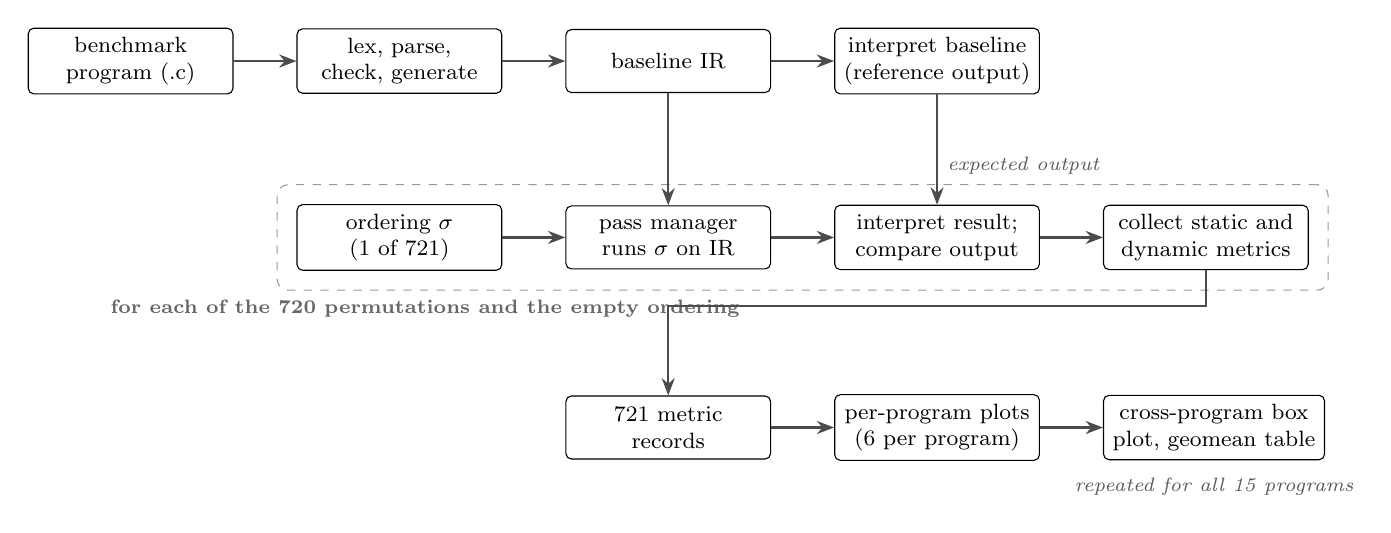
\begin{tikzpicture}[
  font=\footnotesize, node distance=5mm and 8mm,
  stp/.style={draw, rounded corners=2pt, fill=white, minimum height=0.8cm, minimum width=2.6cm, align=center},
  loop/.style={draw=black!40, dashed, rounded corners=4pt, inner sep=7pt},
  arr/.style={-{Stealth[length=2.2mm]}, thick, black!70},
  d/.style={font=\scriptsize\itshape, text=black!65}]
\node[stp] (s1) {benchmark\\program (.c)};
\node[stp, right=of s1] (s2) {lex, parse,\\check, generate};
\node[stp, right=of s2] (s3) {baseline IR};
\node[stp, right=of s3] (s4) {interpret baseline\\(reference output)};
\draw[arr] (s1) -- (s2); \draw[arr] (s2) -- (s3); \draw[arr] (s3) -- (s4);

\node[stp, below=14mm of s2] (l1) {ordering $\sigma$\\(1 of 721)};
\node[stp, right=of l1] (l2) {pass manager\\runs $\sigma$ on IR};
\node[stp, right=of l2] (l3) {interpret result;\\compare output};
\node[stp, right=of l3] (l4) {collect static and\\dynamic metrics};
\draw[arr] (l1) -- (l2); \draw[arr] (l2) -- (l3); \draw[arr] (l3) -- (l4);
\draw[arr] (s3.south) -- ++(0,-0.4) -| (l2.north);
\draw[arr] (s4.south) -- ++(0,-0.4) -| node[d, pos=0.75, right]{expected output} (l3.north);
\begin{scope}[on background layer]
\node[loop, fit=(l1)(l4), label={[font=\scriptsize\bfseries, text=black!60]below left:for each of the 720 permutations and the empty ordering}] {};
\end{scope}

\node[stp, below=16mm of l2] (r1) {721 metric\\records};
\node[stp, right=of r1] (r2) {per-program plots\\(6 per program)};
\node[stp, right=of r2] (r3) {cross-program box\\plot, geomean table};
\draw[arr] (l4.south) -- ++(0,-0.45) -| (r1.north);
\draw[arr] (r1) -- (r2); \draw[arr] (r2) -- (r3);
\node[d, below=1mm of r3] {repeated for all 15 programs};
\end{tikzpicture}}
\caption[High-level design of the exhaustive benchmark workflow.]{High-level design of the exhaustive benchmark workflow. The baseline IR is generated once per program and every ordering is applied to a copy of it. Each result is interpreted and its output compared with the baseline before its metrics are trusted.}
\label{fig:hld-benchmark}
\end{figure}

\textbf{Benchmark workflow.} For each of the fifteen programs, the driver reads the source, runs the front end once to obtain the baseline IR, and interprets the baseline to obtain the reference output. It then iterates over the 721 orderings. For each, it runs the pass manager on a copy of the baseline IR, interprets the optimized IR to obtain the dynamic instruction count, opcode frequencies, and output, compares the output with the reference, and hands the optimized IR and the dynamic results to the metric collector, which returns one record containing the ordering, its label, the static code size, the estimated cycles, the instruction breakdown, the dynamic count, and a correctness flag. After all orderings have been processed the visualizer produces six plots for the program; after all programs, it produces the cross-program box plot and the geometric-mean table, and the driver prints the best ordering per program and warns if any ordering anywhere produced incorrect output. The whole run takes about 24 seconds on the reference machine.

\begin{figure}[!htb]
\centering
\resizebox{\textwidth}{!}{%
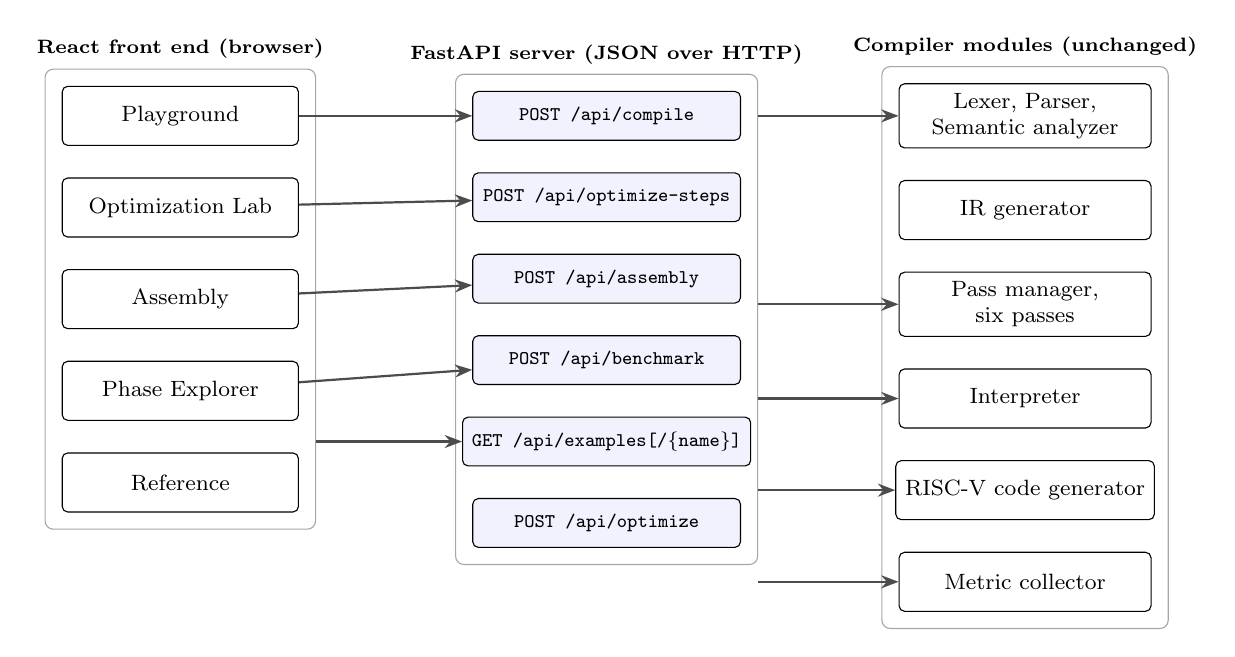
\begin{tikzpicture}[
  font=\footnotesize, node distance=4mm and 10mm,
  box/.style={draw, rounded corners=2pt, fill=white, minimum height=0.75cm, minimum width=3.0cm, align=center},
  ep/.style={draw, rounded corners=2pt, fill=blue!5, minimum height=0.62cm, minimum width=3.4cm, align=left, font=\scriptsize\ttfamily},
  arr/.style={-{Stealth[length=2.2mm]}, thick, black!70},
  grp/.style={draw=black!35, rounded corners=3pt, inner sep=6pt}]
\node[box] (pg) {Playground};
\node[box, below=of pg] (ol) {Optimization Lab};
\node[box, below=of ol] (as) {Assembly};
\node[box, below=of as] (ex) {Phase Explorer};
\node[box, below=of ex] (rf) {Reference};
\begin{scope}[on background layer]
\node[grp, fit=(pg)(rf), label={[font=\scriptsize\bfseries]above:React front end (browser)}] (FE) {};
\end{scope}

\node[ep, right=22mm of pg] (e1) {POST /api/compile};
\node[ep, below=of e1] (e2) {POST /api/optimize-steps};
\node[ep, below=of e2] (e3) {POST /api/assembly};
\node[ep, below=of e3] (e4) {POST /api/benchmark};
\node[ep, below=of e4] (e5) {GET /api/examples[/\{name\}]};
\node[ep, below=of e5] (e6) {POST /api/optimize};
\begin{scope}[on background layer]
\node[grp, fit=(e1)(e6), label={[font=\scriptsize\bfseries]above:FastAPI server (JSON over HTTP)}] (BE) {};
\end{scope}

\node[box, right=20mm of e1, minimum width=3.2cm] (m1) {Lexer, Parser,\\Semantic analyzer};
\node[box, below=of m1, minimum width=3.2cm] (m2) {IR generator};
\node[box, below=of m2, minimum width=3.2cm] (m3) {Pass manager,\\six passes};
\node[box, below=of m3, minimum width=3.2cm] (m4) {Interpreter};
\node[box, below=of m4, minimum width=3.2cm] (m5) {RISC-V code generator};
\node[box, below=of m5, minimum width=3.2cm] (m6) {Metric collector};
\begin{scope}[on background layer]
\node[grp, fit=(m1)(m6), label={[font=\scriptsize\bfseries]above:Compiler modules (unchanged)}] (CM) {};
\end{scope}

\draw[arr] (pg) -- (e1);
\draw[arr] (ol) -- (e2);
\draw[arr] (as) -- (e3);
\draw[arr] (ex) -- (e4);
\draw[arr] (FE.east |- e5) -- (e5);
\draw[arr] (BE.east |- m1) -- (m1);
\draw[arr] (BE.east |- m3) -- (m3);
\draw[arr] (BE.east |- m4) -- (m4);
\draw[arr] (BE.east |- m5) -- (m5);
\draw[arr] (BE.east |- m6) -- (m6);
\end{tikzpicture}}
\caption[High-level design of the interactive web application.]{High-level design of the interactive web application. Each page of the single-page React application calls one primary endpoint; the endpoints are thin adapters that call the same compiler modules the command-line driver uses and serialize the results to JSON.}
\label{fig:hld-web}
\end{figure}

\textbf{Interactive workflow.} The browser loads the React application from the FastAPI server. Each page issues JSON requests to one or two endpoints. The Playground calls \code{/api/compile}, which runs the front end and IR generator and returns tokens, a serialized syntax tree, the symbol list, and the IR both as structured records and as text; on failure it returns a structured error with the phase, message, line, and column, which the editor uses to underline the offending source. The Optimization Lab calls \code{/api/optimize-steps}, which applies the user's ordering one pass at a time and returns, for every stage, the IR text, a line diff against the previous stage, and the metrics. The Assembly page calls \code{/api/assembly}, which returns IR lines, assembly lines, and a mapping between them for hover linking. The Phase Explorer calls \code{/api/benchmark}, which runs all 721 orderings and returns their metrics for plotting in the browser. All pages share the example picker, which lists the fifteen benchmarks grouped by suite through \code{/api/examples}. Because the endpoints call the same modules as the command-line driver, any result seen in the browser is reproducible from the command line.

\section{Detailed Design}

This section describes each component in the order in which data flows through the system. Line counts are given to convey the scale of each module; the complete compiler core is about 4{,}000 lines of Python, the web layer about 1{,}200, the tests about 2{,}000, and the React front end about 1{,}900 lines of TypeScript and CSS.

\subsection{Lexer}

The lexer (\code{compiler/lexer.py}, 268 lines) is a hand-written scanner over the source string. It maintains a position, a line, and a column, and exposes a generator that yields tokens on demand. Each token is an immutable record with a type, the matched text, and the line and column where it began. There are 33 token types: two for literals and identifiers, seven keywords (\code{int}, \code{if}, \code{else}, \code{while}, \code{for}, \code{return}, \code{print}), five arithmetic operators, six comparison operators, three logical operators, assignment, eight delimiters, and an end-of-file marker. Two-character operators are recognized before one-character operators so that \code{<=} is never read as \code{<} followed by \code{=}. Both comment styles are skipped; an unterminated block comment and a digit sequence followed immediately by a letter are reported as lexical errors with the location of the offending construct. The lexer has no knowledge of the grammar and can be run and inspected independently, which the Playground's Tokens tab uses.

\subsection{Parser and abstract syntax tree}

The parser (\code{compiler/parser.py}, 444 lines) is a recursive-descent parser with one method per grammar production. The full grammar is given in Appendix~A. At the top level, a declaration whose third token is a left parenthesis is a function; otherwise it is a global variable. Inside a block, the first token of a statement selects the production: \code{int} for a declaration, which becomes an array declaration if a bracket follows the name; \code{if}, \code{while}, \code{for}, \code{return}, \code{print} for the corresponding statements; a brace for a nested block; and anything else for an assignment or expression statement, which is parsed as an expression and then reinterpreted as an assignment if an \code{=} follows, with the parsed expression required to be an identifier or an array access. An \code{else} followed by \code{if} wraps the nested conditional in an implicit block, giving \code{else if} chains without a dedicated grammar rule. The \code{for} statement allows any of its three clauses to be empty, and its initializer may be a declaration whose scope is the loop.

Expressions are parsed by precedence climbing through six levels: logical or, logical and, equality, comparison, additive, multiplicative, then unary minus and not, then primary expressions, which are integer literals, identifiers, function calls, array accesses, and parenthesized expressions. Every parse error raises an exception carrying the message, the expected construct, and the token actually found, so that a message such as ``Expected RPAREN after if condition (got SEMICOLON `;')'' with a line and column is produced.

The syntax tree (\code{compiler/ast\_nodes.py}, 173 lines) consists of twenty node types defined as Python dataclasses, all carrying a line and column: eight expression nodes (literal, identifier, binary, unary, call, assignment, array access, array assignment), nine statement nodes (variable declaration, array declaration, expression statement, block, if, while, for, return, print), and three top-level nodes (parameter, function declaration, program). The uniform dataclass representation allows the web layer to serialize any tree generically: each node becomes its type name, its scalar fields, and its child nodes in source order.

\subsection{Symbol table and semantic analyzer}

The symbol table (\code{compiler/symbol\_table.py}, 111 lines) is a stack of dictionaries, one per scope. Declaring a name that already exists in the innermost scope is an error; declaring a name that exists in an outer scope is shadowing, and the table assigns the inner variable a unique IR name by appending a counter, so that the flat IR can hold both variables without conflict. Each symbol records its kind (\code{int}, \code{array}, or \code{global}), its scope depth, its IR name, and, for arrays, its element count.

The semantic analyzer (\code{compiler/semantic\_analyzer.py}, 271 lines) runs between parsing and IR generation and enforces the rules listed in Table~\ref{tab:semantic-rules}. It first collects every function's name and arity so that calls may precede definitions, then walks each global and each function body with its own scope stack. Unlike the symbol table, which raises on the first error, the analyzer appends every violation to a list and raises a single exception carrying all of them at the end, so a user sees every problem in one compile. It was added in Phase II after the team observed that Phase I reported such errors from inside IR generation, one at a time and without source positions.

\begin{table}[!htb]
\centering\small
\caption[Rules enforced by the semantic analyzer.]{Rules enforced by the semantic analyzer}
\label{tab:semantic-rules}
\begin{tabular}{L{4.6cm} L{8.6cm}}
\toprule
\textbf{Rule} & \textbf{Reported as}\\
\midrule
Variable declared before use & Undeclared variable `x'\\
No duplicate name in one scope & Variable `x' already declared in this scope\\
Called function exists & Call to undefined function `f'\\
Argument count matches arity & Function `f' expects 2 arguments, got 3\\
No duplicate function definition & Function `f' is defined more than once\\
A \code{main} function exists & No main() function defined\\
Arrays are indexed, scalars are not & `a' is not an array; Array `a' cannot be used as a value\\
Array not assigned without index & Cannot assign to array `a' without an index\\
Global initializer is constant & Global `g' initializer must be a constant expression\\
Global does not shadow a function & Global `f' conflicts with a function of the same name\\
\bottomrule
\end{tabular}
\end{table}

\subsection{Intermediate representation}

The IR (\code{compiler/ir.py}, 253 lines) is a linear three-address code. Each instruction is a record with an opcode and up to three operand strings: a destination and two sources. Operands are variable names, temporary names, label names, or integer literals, and a helper distinguishes literals from names so that passes can treat constants uniformly. The 35 opcodes fall into eight groups, summarized in Table~\ref{tab:opcodes}; the complete reference is in Appendix~B.

\begin{table}[!htb]
\centering\small
\caption[Opcode groups of the three-address code.]{Opcode groups of the three-address code}
\label{tab:opcodes}
\begin{tabular}{L{3.2cm} L{6.0cm} L{3.9cm}}
\toprule
\textbf{Group} & \textbf{Opcodes} & \textbf{Form}\\
\midrule
Arithmetic & ADD, SUB, MUL, DIV, MOD, NEG & \code{d = a op b}, \code{d = -a}\\
Comparison & EQ, NEQ, LT, GT, LTE, GTE & \code{d = a cmp b} (0 or 1)\\
Logical & AND, OR, NOT & \code{d = a \&\& b}, \code{d = !a}\\
Data movement & COPY, LOAD\_CONST & \code{d = a}, \code{d = 5}\\
Control flow & LABEL, JUMP, JUMP\_IF\_TRUE, JUMP\_IF\_FALSE & \code{L:}, \code{goto L}, \code{if a goto L}\\
Functions & PARAM, CALL, RETURN, FUNC\_BEGIN, FUNC\_END, FUNC\_PARAM & \code{param a}, \code{d = call f, n}\\
Memory & ARR\_DECL, ARR\_LOAD, ARR\_STORE, GLOBAL\_DECL, GLOBAL\_LOAD, GLOBAL\_STORE & \code{d = a[i]}, \code{a[i] = v}, \code{d = @g}\\
Other & PRINT, NOP & \code{print a}\\
\bottomrule
\end{tabular}
\end{table}

Two design decisions in the IR are central to the safety of reordering. First, each instruction knows its own \emph{def} and \emph{use} sets: a method returns the variable the instruction writes, if any, and another returns the set of variables it reads, excluding literals. Every pass is written in terms of these two methods rather than in terms of opcodes, so adding an opcode requires updating only these methods for the passes to handle it correctly. Second, memory that outlives a basic block, arrays and global variables, is accessed only through dedicated opcodes. An array store is not a definition of any variable in the def-use sense and a global store is not either, so the local, block-scoped analyses used by the passes can never conclude that such a store is dead or that a value loaded from memory is still available after an intervening store. This is deliberately conservative; it trades some missed optimizations for the guarantee that the passes are correct without alias analysis.

\subsection{IR generator}

The IR generator (\code{compiler/ir\_generator.py}, 352 lines) walks the validated tree and emits instructions. Expressions return the name of the temporary or variable holding their value; literals are materialized with LOAD\_CONST, identifiers return their IR name directly (or a fresh temporary loaded from the global), binary operators emit one instruction into a fresh temporary, and calls emit one PARAM per argument followed by CALL. Control flow is lowered to labels and jumps in the standard way, as shown in Listing~\ref{lst:lowering}. Short-circuit operators are lowered to jumping code: the right operand is evaluated only when the left does not decide the result, and the result is normalized to 0 or 1 with a comparison against zero so that it agrees with the eager AND and OR opcodes. Functions are bracketed by FUNC\_BEGIN and FUNC\_END with one FUNC\_PARAM per parameter, and every variable declared without an initializer is set to zero, matching the zero-initialization of arrays.

\begin{lstlisting}[language=ThreeAC, caption={Lowering patterns used by the IR generator. Left: a while loop. Right: the short-circuit lowering of \code{a \&\& b}, in which \code{b} is evaluated only if \code{a} is true.}, label={lst:lowering}]
while (cond) { body }        |    r = a && b
                              |
L0:                           |      <code for a into ta>
  <code for cond into tc>     |      iffalse ta goto L2
  iffalse tc goto L1          |      <code for b into tb>
  <code for body>             |      r = tb != 0
  goto L0                     |      goto L3
L1:                           |    L2:
                              |      r = 0
                              |    L3:
\end{lstlisting}

\subsection{Interpreter}

The interpreter (\code{compiler/interpreter.py}, 307 lines) executes the IR directly. It indexes labels and function entry points once, then runs \code{main}. Each function call saves the caller's variables and arrays, binds arguments to the callee's FUNC\_PARAM slots, executes until RETURN or FUNC\_END, and restores the caller. Arguments are accumulated from PARAM instructions into a pending list consumed by the next CALL. Arithmetic uses Python integers; division and modulo by zero yield zero rather than raising, and array accesses outside bounds read zero and ignore writes, so that no valid program can crash the interpreter. Every instruction executed, including labels, increments a step counter and a per-opcode frequency table, and a limit of ten million steps guards against non-terminating input. The result record carries the return value, the list of printed integers, the step count, the frequency table, and whether the limit was reached. The step count is the project's dynamic instruction metric, and the printed output is the correctness oracle.

\subsection{Optimization passes}

Each pass lives in its own module under \code{compiler/optimizations/} and exports one function that takes an instruction list and returns a new one. None of them mutate their input. All six are local: they walk the list once (or to a fixed point) and reset any accumulated knowledge at every LABEL, JUMP, conditional jump, CALL, FUNC\_BEGIN, and FUNC\_END, because a value known before a label may be different when control arrives at the label from elsewhere. This is the classical basic-block restriction. It makes the passes weaker than their global counterparts, but it also makes their correctness independent of what ran before them, which is the property that permits arbitrary reordering.

\textbf{Constant folding (CF, 197 lines).} The pass first counts how many times each variable is defined. A variable defined exactly once by a LOAD\_CONST, or by a COPY from a known constant, is entered into a constant map. It then repeatedly substitutes constants into operands and folds any arithmetic, comparison, or logical instruction whose operands are both constant into a LOAD\_CONST, until no instruction changes. A COPY from a constant becomes a LOAD\_CONST; a conditional jump on a constant becomes an unconditional JUMP or a NOP; array and global stores have constants substituted into their operands but are never removed. Division by zero folds to zero, consistent with the interpreter. Because the substitution reaches every instruction, this pass is the principal \emph{enabler} in the system: after it runs, many temporaries that held constants have no remaining readers.

\textbf{Dead code elimination (DCE, 112 lines).} Two sub-passes. First, unreachable code: after an unconditional JUMP or a RETURN, every instruction until the next LABEL, FUNC\_BEGIN, or FUNC\_END is deleted. Second, dead assignments: the pass collects the union of all use sets, deletes every instruction whose defined variable is not in the union and which has no side effect, and repeats until nothing changes, because deleting one instruction can make the instructions that fed it dead in turn. PRINT, RETURN, PARAM, CALL, jumps, labels, array and global stores and declarations are never deleted. DCE is the principal \emph{consumer}: it removes only what other passes have made removable, and it finds almost nothing to do on the baseline IR of most benchmarks, where every temporary is read at least once.

\textbf{Common subexpression elimination (CSE, 158 lines).} The pass maintains a table from expression keys (opcode, first operand, second operand) to the variable holding the result. When an instruction's key is already in the table, the instruction is replaced by a COPY from the earlier result. Two invalidation maps make the table sound: one from each operand to the keys that depend on it, so that redefining an operand removes stale expressions, and one from each result variable to the keys it holds, so that redefining the result variable removes the expressions it used to hold. The second map was added in Phase I after a test exposed a stale-reuse bug. Array loads are excluded from the table because an intervening array store could have changed the element. CSE produces COPY instructions, which are exactly what copy propagation consumes.

\textbf{Copy propagation (CP, 123 lines).} The pass maintains a map from copied variables to their sources, resolving chains transitively. Every subsequent use of a copied variable is replaced by the source, and LOAD\_CONST destinations are entered into the map so that literals propagate as well. Redefining either side of a copy removes the entry. After CP, the COPY instructions themselves are usually dead, and the pass therefore hands work to DCE; it also exposes patterns such as \code{x - x} and \code{a == a} that algebraic simplification can fold, and turns \code{print sum1} into \code{print t18}, which lets DCE remove \code{sum1}.

\textbf{Strength reduction (SR, 166 lines).} A single-instruction rewrite: \code{x * 2} becomes \code{x + x}, \code{x * 1} becomes a COPY, \code{x * 0} and \code{0 / x} become the constant zero, \code{x * -1} becomes NEG, \code{x / 1} and \code{x + 0} and \code{x - 0} become COPY, \code{x \% 1} becomes zero, and \code{x / x}, \code{x \% x}, \code{x - x} become the constants one, zero, and zero. The pass never changes the number of instructions, so it never affects code size; it affects only the cycle estimate (a MUL costing three cycles becomes an ADD costing one) and, through the COPYs it creates, the opportunities available to CP and DCE.

\textbf{Algebraic simplification (AS, 110 lines).} Also a single-instruction rewrite: negation or logical-not of a constant folds to a constant, self-comparisons fold (\code{x == x} to 1, \code{x != x} to 0, \code{x <= x} to 1, and so on), \code{x \&\& 0} folds to 0 and \code{x || k} for non-zero \code{k} folds to 1. Rewrites such as \code{x \&\& 1} to \code{x} were removed in Phase I because they are unsound when \code{x} is not already normalized to 0 or 1. Like SR, AS never changes instruction count.

Listing~\ref{lst:pass-effects} shows the cumulative effect of the best ordering on the \code{main} function of the \code{factorial} benchmark, which was written to exercise all three kinds of opportunity: constant expressions, dead assignments, and a repeated subexpression.

\begin{lstlisting}[language=ThreeAC, caption={The \code{main} function of \code{factorial} before optimization (left, 22 instructions excluding markers) and after CF, CSE, CP, DCE, SR, AS (right, 5 instructions). CF folded \code{base} and \code{extra}; CSE turned the second \code{base + extra} into a copy; CP replaced uses of \code{val}, \code{sum1}, \code{sum2}, \code{t20} by their sources; DCE then removed everything unread.}, label={lst:pass-effects}]
func main:                     |   func main:
  t6 = 2                       |     param 5
  t7 = 3                       |     t12 = call factorial, 1
  t8 = t6 + t7                 |     print t12
  base = t8                    |     print 10
  t9 = 10                      |     print 10
  t10 = 5                      |     return 0
  t11 = t9 - t10               |   end func main
  extra = t11                  |
  param base                   |
  t12 = call factorial, 1      |
  val = t12                    |
  print val                    |
  t13 = 42                     |
  t14 = 2                      |
  t15 = t13 * t14              |
  unused = t15                 |
  t16 = 100                    |
  t17 = unused + t16           |
  also_unused = t17            |
  t18 = base + extra           |
  sum1 = t18                   |
  t19 = base + extra           |
  sum2 = t19                   |
  print sum1                   |
  print sum2                   |
  t20 = 0                      |
  return t20                   |
end func main                  |
\end{lstlisting}

\subsection{Pass manager}

The pass manager (\code{compiler/optimizations/pass\_manager.py}, 107 lines) is deliberately small. It holds a registry mapping the six short names to their functions and a second mapping to their full names. A manager is constructed with a list of names, which it validates, raising a clear error for an unknown name; its \code{run} method copies the input list and folds it through the passes in order; its \code{describe} method renders the ordering as ``Constant Folding -> Common Subexpression Elimination -> \ldots''. Two static methods enumerate orderings: one produces every permutation of every non-empty subset (1{,}956 orderings plus the baseline), and one, used for all reported experiments, produces the 720 full permutations plus the empty ordering. \fig{fig:passmanager} shows the control flow.

\begin{figure}[!htb]
\centering
\resizebox{\textwidth}{!}{%
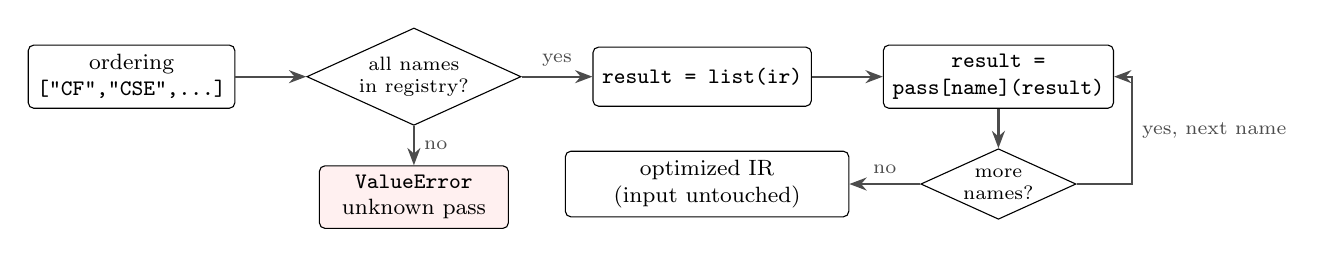
\begin{tikzpicture}[
  font=\footnotesize, node distance=5mm and 9mm,
  box/.style={draw, rounded corners=2pt, fill=white, minimum height=0.75cm, minimum width=2.4cm, align=center},
  dec/.style={draw, diamond, aspect=2.2, fill=white, inner sep=1pt, align=center, font=\scriptsize},
  arr/.style={-{Stealth[length=2.2mm]}, thick, black!70}]
\node[box] (a) {ordering\\\code{["CF","CSE",...]}};
\node[dec, right=of a] (b) {all names\\in registry?};
\node[box, right=of b] (c) {\code{result = list(ir)}};
\node[box, right=of c] (d) {\code{result =}\\\code{pass[name](result)}};
\node[dec, below=of d] (e) {more\\names?};
\node[box, left=of e, minimum width=3.6cm] (f) {optimized IR\\(input untouched)};
\node[box, below=of b, fill=red!6] (g) {\code{ValueError}\\unknown pass};
\draw[arr] (a) -- (b);
\draw[arr] (b) -- node[above, font=\scriptsize]{yes} (c);
\draw[arr] (b) -- node[right, font=\scriptsize]{no} (g);
\draw[arr] (c) -- (d);
\draw[arr] (d) -- (e);
\draw[arr] (e.east) -- ++(0.7,0) |- node[pos=0.25, right, font=\scriptsize]{yes, next name} (d.east);
\draw[arr] (e) -- node[above, font=\scriptsize]{no} (f);
\end{tikzpicture}}
\caption[Control flow of the pass manager.]{Control flow of the pass manager. The input list is copied before the first pass so that the baseline IR can be reused for every ordering; each pass receives the previous pass's output and returns a new list.}
\label{fig:passmanager}
\end{figure}

\subsection{Metric collector}

The metric collector (\code{compiler/benchmarks/metric\_collector.py}, 182 lines) defines the cost model in Table~\ref{tab:cost-model} and three functions over instruction lists. Code size counts instructions excluding labels, NOPs, function markers, parameter declarations, and global declarations, which produce no machine code. The cycle estimate sums the cost of every instruction, including labels at zero cost. The category breakdown counts instructions in eight groups for the stacked-bar plot. The collector combines these with the interpreter's dynamic count and frequency table and the correctness flag into a single record whose label is the ordering rendered as ``CF -> CSE -> \ldots'' or ``Baseline (none)''.

\begin{table}[!htb]
\centering\small
\caption[Per-instruction cost model used for the estimated-cycle metric (ARM Cortex-M class).]{Per-instruction cost model used for the estimated-cycle metric (ARM Cortex-M class)}
\label{tab:cost-model}
\begin{tabular}{L{7.4cm} C{2.2cm} L{3.6cm}}
\toprule
\textbf{Opcodes} & \textbf{Cost} & \textbf{Rationale}\\
\midrule
ADD, SUB, NEG, comparisons, AND, OR, NOT, COPY, LOAD\_CONST, PARAM & 1 & single-cycle ALU or move\\
MUL & 3 & multi-cycle multiplier\\
DIV, MOD & 12 & iterative hardware divider\\
JUMP, JUMP\_IF\_TRUE, JUMP\_IF\_FALSE & 2 & branch penalty\\
ARR\_LOAD, ARR\_STORE, GLOBAL\_LOAD, GLOBAL\_STORE & 2 & load/store\\
CALL & 5 & call overhead, register save\\
RETURN & 3 & return overhead\\
PRINT & 10 & output routine\\
LABEL, NOP, FUNC\_BEGIN, FUNC\_END, FUNC\_PARAM, ARR\_DECL, GLOBAL\_DECL & 0 & no code emitted\\
\bottomrule
\end{tabular}
\end{table}

\subsection{Visualizer}

The visualizer (\code{compiler/benchmarks/visualizer.py}, 560 lines) produces seven plot types with matplotlib: a scatter of code size against estimated cycles with the Pareto front overlaid; bars of size and cycles normalized to the baseline; a pairwise pass-interaction heatmap whose cell $(A, B)$ is the mean code size of orderings with $A$ before $B$ minus that of orderings with $B$ before $A$; stacked bars of the instruction-category breakdown; a heatmap of percentage reduction in all three metrics; paired bars of static against dynamic count; and a cross-program box plot of code-size reduction. Because hundreds of orderings produce identical outcomes, the scatter and reduction heatmap group orderings by outcome and plot one point or column per distinct outcome, labelled with a representative ordering and the number of orderings sharing it; this de-duplication was added in Phase II after the full-permutation plots became illegible. The module also computes the geometric-mean summary across programs.

\subsection{RISC-V back end and simulator}

The code generator (\code{compiler/codegen\_riscv.py}, 520 lines) lowers the IR to RV32IM assembly in GNU syntax for Linux user mode. It follows the classical course-compiler strategy: every variable, temporary, and array in a function receives a slot in the stack frame; operands are loaded into \code{t0} and \code{t1}, the result is computed into \code{t2}, and stored back. The frame layout is shown in \fig{fig:frame}. The return address and the caller's frame pointer are saved at the top of the frame, scalars follow at 4-byte offsets below the frame pointer, arrays follow the scalars, and the frame is rounded up to a multiple of 16 bytes as the RISC-V calling convention requires. Arguments are passed in \code{a0}--\code{a7}, so functions with more than eight parameters are rejected with a clear error. Offsets beyond the 12-bit immediate range are addressed through a scratch register.

\begin{figure}[!htb]
\centering
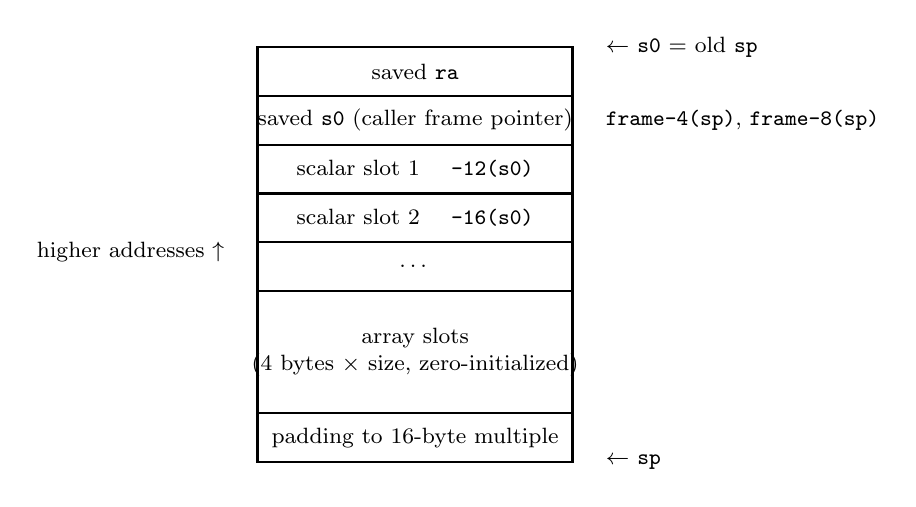
\begin{tikzpicture}[font=\footnotesize, yscale=0.62]
\draw[thick] (0,0) rectangle (4,1); \node at (2,0.5) {saved \code{ra}};
\draw[thick] (0,-1) rectangle (4,0); \node at (2,-0.5) {saved \code{s0} (caller frame pointer)};
\draw[thick] (0,-2) rectangle (4,-1); \node at (2,-1.5) {scalar slot 1 \quad \code{-12(s0)}};
\draw[thick] (0,-3) rectangle (4,-2); \node at (2,-2.5) {scalar slot 2 \quad \code{-16(s0)}};
\draw[thick] (0,-4) rectangle (4,-3); \node at (2,-3.5) {\ldots};
\draw[thick] (0,-6.5) rectangle (4,-4); \node[align=center] at (2,-5.25) {array slots\\(4 bytes $\times$ size, zero-initialized)};
\draw[thick] (0,-7.5) rectangle (4,-6.5); \node at (2,-7) {padding to 16-byte multiple};
\node[anchor=west] at (4.3,1) {$\leftarrow$ \code{s0} = old \code{sp}};
\node[anchor=west] at (4.3,-7.5) {$\leftarrow$ \code{sp}};
\node[anchor=west] at (4.3,-0.5) {\code{frame-4(sp)}, \code{frame-8(sp)}};
\node[anchor=east] at (-0.3,-3.2) {higher addresses $\uparrow$};
\end{tikzpicture}
\caption[Stack frame layout produced by the RISC-V back end for one function.]{Stack frame layout produced by the RISC-V back end for one function. Every IR name in the function receives a slot; no register allocation is performed.}
\label{fig:frame}
\end{figure}

Three semantic details are handled explicitly so that the assembly behaves exactly like the interpreter. Division and modulo are guarded by a branch that yields zero when the divisor is zero, because the hardware instructions would return $-1$ or the dividend. Comparisons are lowered to \code{slt}, \code{seqz}, \code{snez}, and \code{xori} sequences producing 0 or 1. Printing calls a built-in \code{print\_int} routine, emitted once per module, that converts a signed integer to decimal in a stack buffer and issues the Linux \code{write} system call; the program exits through the \code{exit} system call with \code{main}'s return value as status. Global variables are placed in a \code{.data} section and accessed with \code{la}/\code{lw}/\code{sw}. The generator also records, for every IR instruction, the range of assembly lines it produced, which the Assembly page uses for hover linking.

The simulator (\code{tests/riscv\_sim.py}, 213 lines) is a test oracle, not a general emulator. It parses exactly the instruction subset the generator emits, executes it with 32-bit wrap-around arithmetic, implements the two system calls, and captures standard output. A test compiles every benchmark under the best ordering and under no optimization, generates assembly, runs it in the simulator, and asserts that the printed integers and exit code equal the interpreter's. This closes the loop: an improvement measured on the IR is only reported if the lowered program still computes the same result.

\subsection{Web API and front end}

The FastAPI application (\code{compiler/web/app.py}, 495 lines, with Pydantic models in \code{api\_models.py}) exposes the endpoints in Table~\ref{tab:endpoints}. Every compile-like endpoint runs the front end and returns either the requested artefacts or a structured error record naming the phase (lexer, parser, semantic, IR generator, optimization, or runtime), the message, and the source line and column when known. Example names are validated against a strict pattern and resolved inside the benchmark directory only, so the file-serving endpoint cannot be used to read arbitrary files. The examples endpoint classifies each program as MiBench or PolyBench from its documentation comment and extracts that comment into a title and bullet points so the front end can present it.

\begin{table}[!htb]
\centering\small
\caption[HTTP endpoints exposed by the FastAPI server.]{HTTP endpoints exposed by the FastAPI server}
\label{tab:endpoints}
\begin{tabular}{L{4.3cm} L{8.9cm}}
\toprule
\textbf{Endpoint} & \textbf{Returns}\\
\midrule
\code{POST /api/compile} & tokens, serialized AST, symbols, IR records and text\\
\code{POST /api/optimize} & optimized IR, line diff, metrics, output, correctness, assembly\\
\code{POST /api/optimize-steps} & one stage per pass: IR text, diff against previous stage, size, cycles\\
\code{POST /api/assembly} & IR lines, assembly lines, IR-to-assembly line mapping\\
\code{POST /api/benchmark} & metrics for all 721 orderings and the baseline\\
\code{GET /api/examples} & name, description, and suite of each benchmark\\
\code{GET /api/examples/\{name\}} & source and structured documentation of one benchmark\\
\code{GET /}, \code{GET /legacy} & the React application; the zero-dependency legacy page\\
\bottomrule
\end{tabular}
\end{table}

The front end (\code{frontend/}, React 19 and TypeScript) is a single-page application with a sidebar and five pages. A typed API client mirrors the endpoint schemas. The shared editor component wraps CodeMirror 6 with a C language mode and a lint source that converts the server's error record into an underline at the reported position. A pipeline-rail component shows which stages of the pipeline a page exercises. The Playground compiles on load and offers tabs for tokens, a collapsible syntax tree, the symbol table, and the IR. The Optimization Lab presents the six passes as chips that can be dragged, or moved with the arrow keys for keyboard users, runs the ordering stage by stage, and shows the IR after any selected stage with removed lines struck through and added lines highlighted, together with the size and cycle deltas. The Assembly page shows IR and assembly side by side and highlights the assembly lines that correspond to the IR line under the cursor. The Phase Explorer runs all orderings and draws a scatter of size against cycles with the Pareto frontier highlighted and a bar chart of the ten smallest results; clicking a point reveals its ordering and metrics. The Reference page documents the passes, cost model, language, and pipeline. The build output is committed under \code{compiler/web/static/} so that the server works from a fresh clone without a JavaScript toolchain, and all fonts are bundled so the application works offline.

\subsection{Development history}

Table~\ref{tab:milestones} summarizes the development milestones as recorded in version control. The project was developed in two concentrated phases with a hardening step between them; 54 commits were made in total.

\begin{table}[!htb]
\centering\small
\caption[Development milestones recorded in version control.]{Development milestones recorded in version control}
\label{tab:milestones}
\begin{tabular}{L{2.4cm} L{10.8cm}}
\toprule
\textbf{Date} & \textbf{Milestone}\\
\midrule
11 Feb 2026 & Repository created; project proposal with the four-phase plan.\\
14 Apr 2026 & Design specification and implementation plan for the interactive tool. Lexer, parser, symbol table, IR, IR generator, interpreter, six passes, pass manager, metric collector, visualizer, eight MiBench-adapted benchmarks, command-line driver, single-file web UI, and first test suite delivered in one integration.\\
15--16 Apr 2026 & Hardening: fixed stale reuse in CSE, removed unsound boolean rewrites in AS, hardened the examples endpoint against path traversal, fixed the pass-interaction heatmap to use full-ordering data, added repository ignore rules.\\
5 Aug 2026 & Arrays added end to end: bracket tokens, AST nodes, symbol-table sizes, parsing, IR opcodes, IR generation, interpretation, array-aware passes, tests. Seven PolyBench-adapted array benchmarks added with documentation. Array cost model. Semantic analyzer, global variables, \code{for} loops, \code{else if}, short-circuit evaluation, shared error hierarchy, RISC-V RV32IM back end with simulator and 44 new tests. Web UI rebuilt as a React application with stepping, assembly, and explorer pages; examples grouped by suite. Documentation brought up to date.\\
6 Aug 2026 & Plot de-duplication for full-permutation datasets with regression tests; final benchmark plots regenerated.\\
\bottomrule
\end{tabular}
\end{table}

\section{Benchmark Dataset Description}

The dataset for this study is a suite of fifteen programs written in the supported C subset. Each is an adaptation of a kernel from a published benchmark suite, chosen so that the suite covers the control-flow and data-access patterns typical of embedded software (MiBench) and of numerical loop nests (PolyBench/C). The programs live in \code{compiler/benchmarks/programs/}, one file each, and every file begins with a documentation comment naming its source and the optimization opportunities it was designed to exercise. Table~\ref{tab:benchmarks} lists them with their baseline sizes.

\begin{table}[!htb]
\centering\small
\caption[The fifteen benchmark programs.]{The fifteen benchmark programs. Size is the static instruction count of the unoptimized IR; dynamic is the number of IR instructions executed by the interpreter.}
\label{tab:benchmarks}
\begin{tabular}{L{1.7cm} L{4.2cm} L{4.6cm} C{1.0cm} C{1.4cm}}
\toprule
\textbf{Program} & \textbf{Source kernel} & \textbf{Characteristic} & \textbf{Size} & \textbf{Dynamic}\\
\midrule
bitcount & MiBench automotive/bitcnts & loop, conditional, div/mod as shift/mask & 33 & 354\\
collatz & MiBench automotive patterns & unpredictable branching, mixed arithmetic & 42 & 4{,}712\\
factorial & MiBench basicmath & multiplication loop, planted dead code and CSE & 40 & 81\\
fibonacci & MiBench basicmath & iterative loop, rotating variable updates & 22 & 236\\
gcd & MiBench basicmath & Euclid's algorithm, modulo in loop & 21 & 45\\
isqrt & MiBench automotive/basicmath & Newton iteration, division-heavy & 50 & 347\\
power & MiBench security/blowfish & square-and-multiply modular exponentiation & 71 & 511\\
sha\_mix & MiBench security/sha & nested conditionals, modular mixing rounds & 106 & 2{,}522\\
jacobi1d & PolyBench stencils/jacobi-1d & array load/store, $i\pm1$ indexing, time steps & 76 & 1{,}064\\
jacobi2d & PolyBench stencils/jacobi-2d & flattened 2-D grid, five-point stencil & 144 & 2{,}787\\
gemm & PolyBench blas/gemm & triple loop, multiply-accumulate into array & 164 & 3{,}081\\
2mm & PolyBench kernels/2mm & two chained matrix products, five live arrays & 252 & 5{,}259\\
atax & PolyBench kernels/atax & two reductions sharing an intermediate array & 101 & 1{,}448\\
bicg & PolyBench kernels/bicg & two accumulators from one shared load & 94 & 1{,}283\\
gesummv & PolyBench blas/gesummv & two matrix-vector products plus scalar combine & 106 & 1{,}487\\
\bottomrule
\end{tabular}
\end{table}

\textbf{Adaptation rules.} The source language has no bitwise operators, no floating point, no two-dimensional arrays, and no input. The kernels were adapted under four rules. Bit operations are expressed with division and modulo by two, which are semantically identical for non-negative operands (\code{bitcount}). Floating-point kernels are made integer, with divisions used where the original averaged (\code{jacobi1d}, \code{jacobi2d}). Two-dimensional arrays are flattened to one dimension with explicit row-major index arithmetic \code{a[i * n + j]}, which is faithful to how a C compiler lays them out and which produces exactly the repeated index expressions that common subexpression elimination and strength reduction target. Inputs are fixed to small constant problem sizes (matrices of $4\times4$ or $5\times5$, vectors of 5 or 8 elements, a handful of time steps) initialized by simple arithmetic formulas, and results are printed so that the interpreter's output is a complete witness of the computation; every printed value participates in a checksum that is also returned. Listing~\ref{lst:jacobi1d} shows one adapted kernel in full.

\begin{lstlisting}[language=CSubset, caption={The \code{jacobi1d} benchmark, adapted from PolyBench/C stencils/jacobi-1d. Two buffers alternate over four time steps; each interior element becomes the integer mean of itself and its two neighbours.}, label={lst:jacobi1d}]
int main() {
    int n = 8;
    int steps = 4;
    int a[8];
    int b[8];

    int i = 0;
    while (i < n) {
        a[i] = (i * i) % 7 + 1;
        i = i + 1;
    }

    int t = 0;
    while (t < steps) {
        i = 1;
        while (i < n - 1) {
            b[i] = (a[i - 1] + a[i] + a[i + 1]) / 3;
            i = i + 1;
        }
        i = 1;
        while (i < n - 1) {
            a[i] = b[i];
            i = i + 1;
        }
        t = t + 1;
    }

    i = 0;
    while (i < n) {
        print(a[i]);
        i = i + 1;
    }
    return a[n / 2];
}
\end{lstlisting}

\textbf{Coverage.} The eight MiBench-derived programs are scalar: they exercise function calls, loops with data-dependent trip counts, conditionals, and integer arithmetic including expensive division and modulo. Two of them (\code{factorial} and \code{sha\_mix}) contain planted dead code and repeated subexpressions so that every pass has visible work on at least one program. The seven PolyBench-derived programs are array-based: they exercise array loads and stores, repeated affine index arithmetic, and deep loop nests, and they contain no planted opportunities; whatever the passes find in them is what a compiler would find in real numerical code. The two groups behave measurably differently under optimization, as Chapter 5 shows.

\section{Tools and Technologies used for Implementation}

\begin{itemize}
  \item \textbf{Python 3.12.} The compiler, interpreter, passes, back end, benchmark driver, and web server are written in Python with type annotations and dataclasses throughout. Python was chosen for readability, since the code is meant to be read by students, and for speed of development; its performance is more than sufficient, since the full 10{,}815-compilation benchmark runs in about 24 seconds.
  \item \textbf{FastAPI 0.141, Uvicorn 0.52, Pydantic 2.} The web server. FastAPI provides typed request and response models, automatic validation, and an interactive API description; Uvicorn is the ASGI server. The server serves both the JSON API and the static front end from one process.
  \item \textbf{React 19, TypeScript 6, Vite 8.} The front end. React components map naturally onto the pages and shared widgets; TypeScript's types mirror the Pydantic models so that API changes are caught at build time; Vite builds the application into the static directory served by FastAPI.
  \item \textbf{CodeMirror 6.} The source editor, with the C language mode for highlighting and the lint extension for underlining compiler errors at their reported positions.
  \item \textbf{Chart.js 4 with react-chartjs-2.} Interactive scatter and bar charts in the Phase Explorer, with hover tooltips and click-to-select.
  \item \textbf{matplotlib 3.11 and NumPy 1.26.} Publication-quality static plots from the benchmark driver, rendered headlessly with the Agg back end.
  \item \textbf{pytest 9.} The test framework; 185 test cases in three modules, including parametrized end-to-end tests over all benchmarks and all orderings.
  \item \textbf{RISC-V GNU toolchain and QEMU (optional).} The generated assembly is written for \code{riscv64-linux-gnu-gcc -march=rv32im -mabi=ilp32} and \code{qemu-riscv32}; they are not required because the bundled simulator validates the assembly in the test suite.
  \item \textbf{Git and GitHub.} Version control and collaboration; the repository history is summarized in Table~\ref{tab:milestones}.
  \item \textbf{Visual Studio Code, Linux Mint 22.2, Windows.} Development environments. The system runs unchanged on both operating systems.
  \item \textbf{Bundled fonts: Inter, JetBrains Mono, Space Grotesk.} Packaged with the front end so the application has no network dependency.
\end{itemize}

\chapter{Results and Discussion}

\section{Experimentation Environment Set Up}

All experiments reported in this chapter were produced by a single command, \code{python -m compiler.main --benchmark-all}, which compiles each of the fifteen benchmark programs under all 721 orderings, interprets every result, and writes the metrics, plots, and geometric-mean summary. The command is deterministic: the compiler uses no randomness, no timing, and no floating-point arithmetic in any decision, so repeated runs on any machine produce byte-identical intermediate code, assembly, and metric tables. The interactive results in Section~\ref{sec:gui} were produced by the same modules through the web application.

\begin{itemize}
  \item \textbf{Reference machine:} AMD Ryzen 7 7435HS (8 cores, 16 threads), 24 GB RAM, solid-state storage.
  \item \textbf{Operating system:} Linux Mint 22.2 (kernel 6.17). The system was also exercised on Windows during development; results are identical.
  \item \textbf{Runtime:} Python 3.12.3; NumPy 1.26.4; matplotlib 3.11.0; FastAPI 0.141.1; Uvicorn 0.52.1; Pydantic 2.13.4; pytest 9.1.1.
  \item \textbf{Front end build:} Node.js 20, Vite 8, TypeScript 6, React 19; the built bundle is committed and was served unchanged.
  \item \textbf{Browser for screenshots:} Chromium, 1440 $\times$ 900 viewport at 2$\times$ device scale.
  \item \textbf{Repository state:} commit \code{bce09e6} (6 August 2026) of the project repository, 54 commits, all 185 tests passing.
\end{itemize}

The exhaustive benchmark of all fifteen programs, 10{,}815 compile-and-execute runs plus plot generation, completed in 23.5 seconds. Per-program times range from 0.17 seconds for \code{gcd} to 5.21 seconds for \code{2mm}, the largest program at 252 baseline instructions and 5{,}259 executed instructions; the time is dominated by interpreting the 721 optimized programs, not by optimizing them. The full test suite completed in 3.98 seconds.

\section{Functional Requirements Results Achieved}

All twelve functional requirements defined in Chapter 3 were achieved. Table~\ref{tab:fr-status} records the status of each together with the evidence that establishes it.

\begin{table}[!htb]
\centering\small
\caption{Functional Requirements Status Table}
\label{tab:fr-status}
\begin{tabular}{L{1.4cm} L{5.0cm} L{1.6cm} L{5.2cm}}
\toprule
\textbf{FR} & \textbf{Functional requirement} & \textbf{Status} & \textbf{Evidence}\\
\midrule
FR-1 & Lexical analysis with positions and comment handling & Achieved & \code{TestLexer} (12 cases); Tokens tab in Playground\\
FR-2 & Recursive-descent parsing with precedence and located errors & Achieved & \code{TestParser}, \code{TestElseIf}, \code{TestForLoop}; AST tab\\
FR-3 & Semantic analysis collecting all violations & Achieved & \code{TestSemanticAnalyzer} (14 cases); editor underlines\\
FR-4 & Three-address code generation incl.\ arrays, globals, short-circuit & Achieved & \code{TestIRGenerator}, \code{TestArrays}, \code{TestGlobals}, \code{TestShortCircuit}\\
FR-5 & IR interpretation with dynamic counts and step limit & Achieved & \code{TestInterpreter} (9 cases)\\
FR-6 & Six correct, reorderable passes & Achieved & pass unit tests (33 cases); output equality on 10{,}815 runs\\
FR-7 & Pass manager with validation and full enumeration & Achieved & \code{TestPassManager}; 721 orderings per program\\
FR-8 & Static size, cycle estimate, category breakdown & Achieved & \code{TestMetrics} (6 cases)\\
FR-9 & Exhaustive benchmark with plots and geomean & Achieved & 91 plots and summary table generated; Section~\ref{sec:empirical}\\
FR-10 & RISC-V RV32IM generation with line mapping & Achieved & \code{TestRiscvBackend} (9 cases); all benchmarks match interpreter in simulator\\
FR-11 & Interactive web application (five pages) & Achieved & \code{test\_web.py} (24 cases); Section~\ref{sec:gui}\\
FR-12 & Command-line interface & Achieved & all flags exercised in this chapter\\
\bottomrule
\end{tabular}
\end{table}

\subsection*{Empirical results of the phase-ordering study}
\label{sec:empirical}

The remainder of this section presents the results that FR-9 produces, which are the scientific content of the project.

\subsubsection*{Effect of the best ordering on each program}

Table~\ref{tab:per-program} gives, for every program, the baseline metrics and the metrics of the best ordering, and \fig{fig:reduction-by-program} shows the reductions graphically. The best ordering is the same for every program: \ordering{CF $\to$ CSE $\to$ CP $\to$ DCE $\to$ SR $\to$ AS}, or any of the 29 other orderings equivalent to it (see below). It minimizes all three metrics simultaneously on all fifteen programs; there is no program on which the smallest code is not also the cheapest code.

\begin{table}[!htb]
\centering\small
\caption{Baseline and best-ordering metrics for each program}
\label{tab:per-program}
\begin{tabular}{L{1.7cm} C{0.9cm} C{0.9cm} C{1.15cm} C{0.95cm} C{0.95cm} C{1.15cm} C{1.05cm} C{1.05cm} C{1.15cm}}
\toprule
 & \multicolumn{3}{c}{\textbf{Static size}} & \multicolumn{3}{c}{\textbf{Est.\ cycles}} & \multicolumn{3}{c}{\textbf{Dynamic count}}\\
\cmidrule(lr){2-4}\cmidrule(lr){5-7}\cmidrule(lr){8-10}
\textbf{Program} & base & best & red.\ \% & base & best & red.\ \% & base & best & red.\ \%\\
\midrule
factorial & 40 & 16 & 60.0 & 81 & 55 & 32.1 & 81 & 53 & 34.6\\
isqrt & 50 & 27 & 46.0 & 153 & 120 & 21.6 & 347 & 294 & 15.3\\
bitcount & 33 & 19 & 42.4 & 88 & 74 & 15.9 & 354 & 235 & 33.6\\
fibonacci & 22 & 13 & 40.9 & 35 & 26 & 25.7 & 236 & 189 & 19.9\\
collatz & 42 & 26 & 38.1 & 113 & 97 & 14.2 & 4{,}712 & 3{,}193 & 32.2\\
sha\_mix & 106 & 68 & 35.8 & 255 & 217 & 14.9 & 2{,}522 & 1{,}897 & 24.8\\
jacobi1d & 76 & 50 & 34.2 & 139 & 102 & 26.6 & 1{,}064 & 755 & 29.0\\
jacobi2d & 144 & 95 & 34.0 & 251 & 166 & 33.9 & 2{,}787 & 2{,}053 & 26.3\\
power & 71 & 47 & 33.8 & 202 & 178 & 11.9 & 511 & 378 & 26.0\\
gcd & 21 & 14 & 33.3 & 51 & 44 & 13.7 & 45 & 35 & 22.2\\
gemm & 164 & 119 & 27.4 & 268 & 211 & 21.3 & 3{,}081 & 2{,}591 & 15.9\\
2mm & 252 & 185 & 26.6 & 401 & 316 & 21.2 & 5{,}259 & 4{,}420 & 16.0\\
gesummv & 106 & 78 & 26.4 & 180 & 144 & 20.0 & 1{,}487 & 1{,}207 & 18.8\\
atax & 101 & 78 & 22.8 & 157 & 134 & 14.6 & 1{,}448 & 1{,}261 & 12.9\\
bicg & 94 & 73 & 22.3 & 159 & 134 & 15.7 & 1{,}283 & 1{,}082 & 15.7\\
\midrule
\textbf{Geometric mean ratio} & & & \textbf{0.6426} & & & \textbf{0.7950} & & & \textbf{0.7679}\\
\bottomrule
\end{tabular}
\end{table}

\begin{figure}[!htb]
\centering
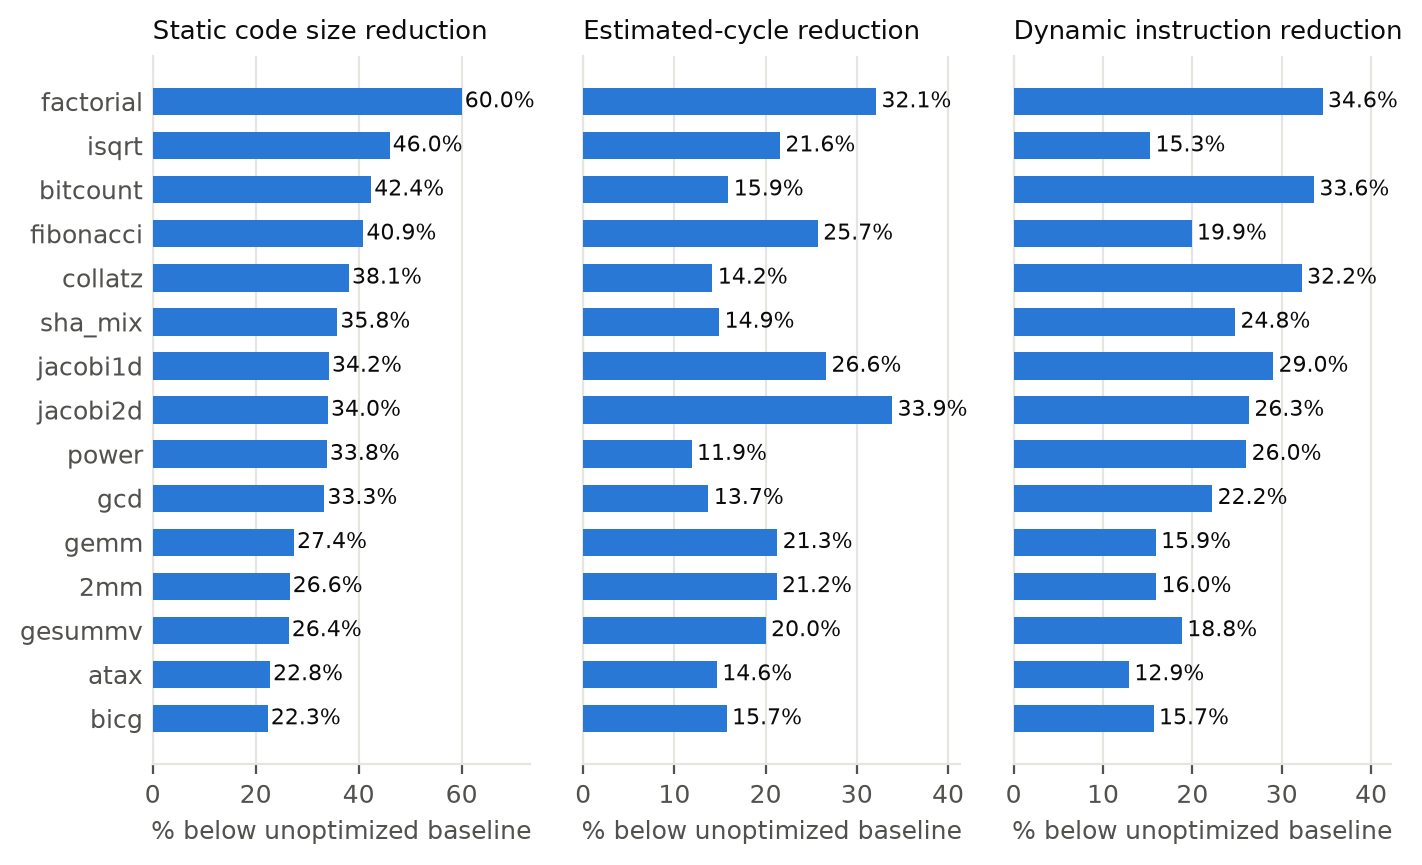
\includegraphics[width=\textwidth]{fig_reduction_by_program}
\caption[Reductions achieved by the best ordering on each program.]{Reductions achieved by the best ordering on each program, relative to the unoptimized baseline, for the three metrics. Programs are sorted by code-size reduction. The eight scalar MiBench-derived kernels occupy the top of the size ranking; the seven array-based PolyBench-derived kernels occupy the bottom.}
\label{fig:reduction-by-program}
\end{figure}

Across the fifteen programs the best ordering reduces static code size by a geometric mean of 35.7\%, the estimated cycle cost by 20.5\%, and the dynamic instruction count by 23.2\%. The size reduction ranges from 22.3\% on \code{bicg} to 60.0\% on \code{factorial}. Two groups are visible. The scalar MiBench-derived programs are reduced by 33\% to 60\% in size; the array-based PolyBench-derived programs by 22\% to 34\%. The reason is structural. In the scalar kernels, a large fraction of the baseline instructions are temporaries that hold literals (\code{t4 = 1} before \code{t5 = i + t4}) or copies from temporaries into named variables (\code{result = t0}); constant folding and copy propagation make those temporaries unread and dead code elimination removes them. In the array kernels, the loop bodies are dominated by array loads and stores and by index arithmetic on loop variables that are reassigned every iteration. Neither can be removed: memory operations are never deleted without alias analysis, and a variable that is assigned more than once is not a candidate for constant propagation. What remains removable in those kernels is the same class of literal-holding temporaries, which is a smaller share of the whole.

The cycle reductions are smaller than the size reductions everywhere except \code{jacobi2d}, and are smallest on the division-heavy programs \code{power} (11.9\%) and \code{gcd} (13.7\%). Division and modulo cost twelve cycles each in the model and are never eliminated, since their operands are loop-carried, so they dominate the cycle estimate before and after optimization. The dynamic reductions are large on the loop-heavy scalar programs (\code{bitcount} 33.6\%, \code{collatz} 32.2\%) because a single instruction removed from a loop body is removed from every iteration.

\fig{fig:box} shows the distribution of code-size reduction across all 720 orderings for each program. The boxes are narrow because most orderings fall into a few classes; the whiskers reach zero on thirteen programs because the worst orderings achieve nothing at all.

\begin{figure}[!htb]
\centering
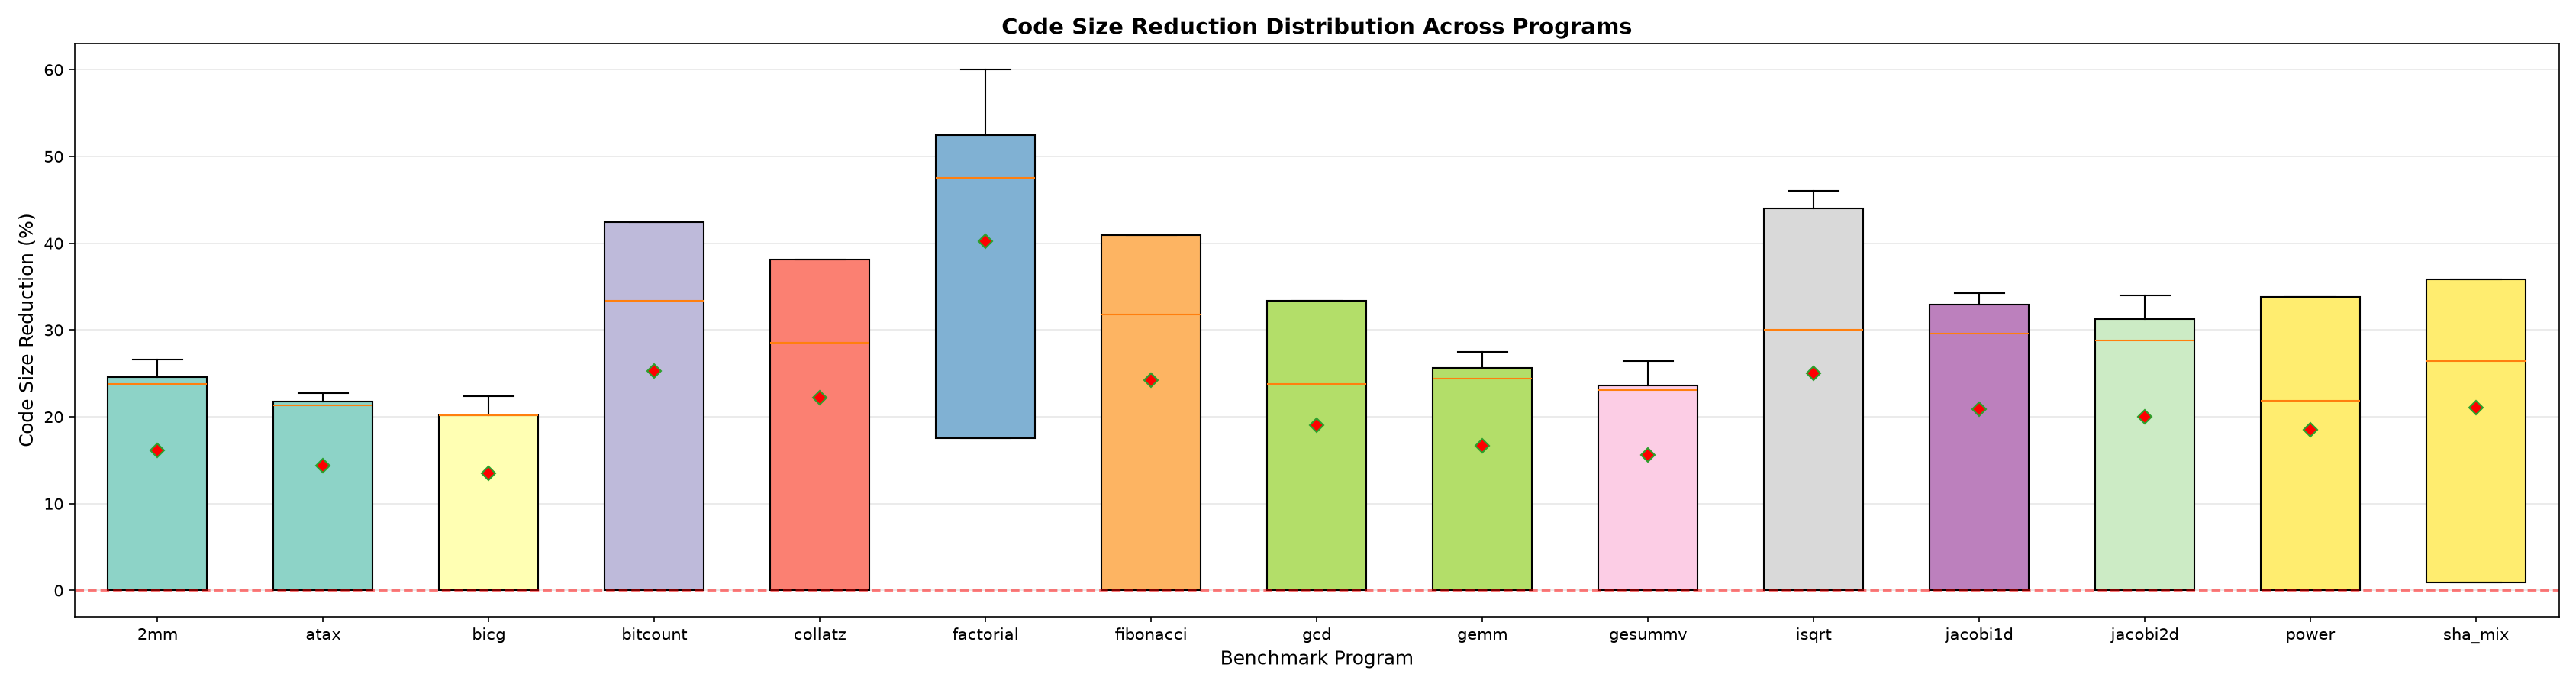
\includegraphics[width=\textwidth]{cross_program_box}
\caption[Distribution of code-size reduction across all 720 orderings, per program.]{Distribution of code-size reduction across all 720 orderings for each program, produced by the visualizer. Red diamonds mark the mean. The lower whisker touches zero on every program except \code{factorial} and \code{sha\_mix}, the two programs with planted dead code that DCE can remove without help.}
\label{fig:box}
\end{figure}

\subsubsection*{Aggregate effect of every ordering}

Aggregating with the geometric mean over the fifteen programs, the 720 orderings produce only nine distinct code-size outcomes, listed in Table~\ref{tab:classes} and plotted in \fig{fig:geomean-classes}. Each outcome is an \emph{equivalence class} of orderings that produce identical code on every program. The classes are determined entirely by the relative order of four passes, constant folding, common subexpression elimination, copy propagation, and dead code elimination; the positions of strength reduction and algebraic simplification are irrelevant to code size. The $4! = 24$ relative orders of the four passes each contain $720/24 = 30$ orderings, and the 24 relative orders map onto nine size classes, which is why the class sizes in the table are multiples of 30.

\begin{table}[!htb]
\centering\small
\caption{The nine equivalence classes of orderings, by geometric-mean normalized code size}
\label{tab:classes}
\begin{tabular}{C{0.7cm} L{6.3cm} C{1.2cm} C{1.1cm} C{1.7cm} C{1.2cm}}
\toprule
\textbf{Class} & \textbf{Relative order of CF, CSE, CP, DCE (one representative)} & \textbf{Orderings} & \textbf{Size ratio} & \textbf{Cycle ratio (range)} & \textbf{Dynamic ratio}\\
\midrule
1 & CF $\to$ CSE $\to$ CP $\to$ DCE & 30 & 0.6426 & 0.7950--0.7999 & 0.7679\\
2 & CSE $\to$ CF $\to$ CP $\to$ DCE & 30 & 0.6459 & 0.7984--0.8033 & 0.7729\\
3 & CF $\to$ CP $\to$ CSE $\to$ DCE (and CF, CP, DCE, CSE) & 60 & 0.6507 & 0.8006--0.8055 & 0.7820\\
4 & CSE $\to$ CP $\to$ CF $\to$ DCE & 30 & 0.6526 & 0.8007--0.8056 & 0.7750\\
5 & CP $\to$ CF $\to$ CSE $\to$ DCE (and two others with CP first, DCE after CF) & 90 & 0.6598 & 0.8039--0.8099 & 0.7850\\
6 & CSE $\to$ CP $\to$ DCE $\to$ CF & 30 & 0.6844 & 0.8179--0.8227 & 0.7866\\
7 & CP $\to$ CSE $\to$ DCE $\to$ CF (and two others with CP first, DCE before CF) & 90 & 0.6913 & 0.8210--0.8269 & 0.7965\\
8 & CF $\to$ CSE $\to$ DCE $\to$ CP (and three others in which CF precedes DCE and DCE precedes CP) & 120 & 0.7526 & 0.8393--0.8456 & 0.8147\\
9 & DCE before both CF and CP (eight relative orders) & 240 & 0.9866 & 0.9615--0.9675 & 0.9940\\
\midrule
 & Baseline (no optimization) & 1 & 1.0000 & 1.0000 & 1.0000\\
\bottomrule
\end{tabular}
\end{table}

\begin{figure}[!htb]
\centering
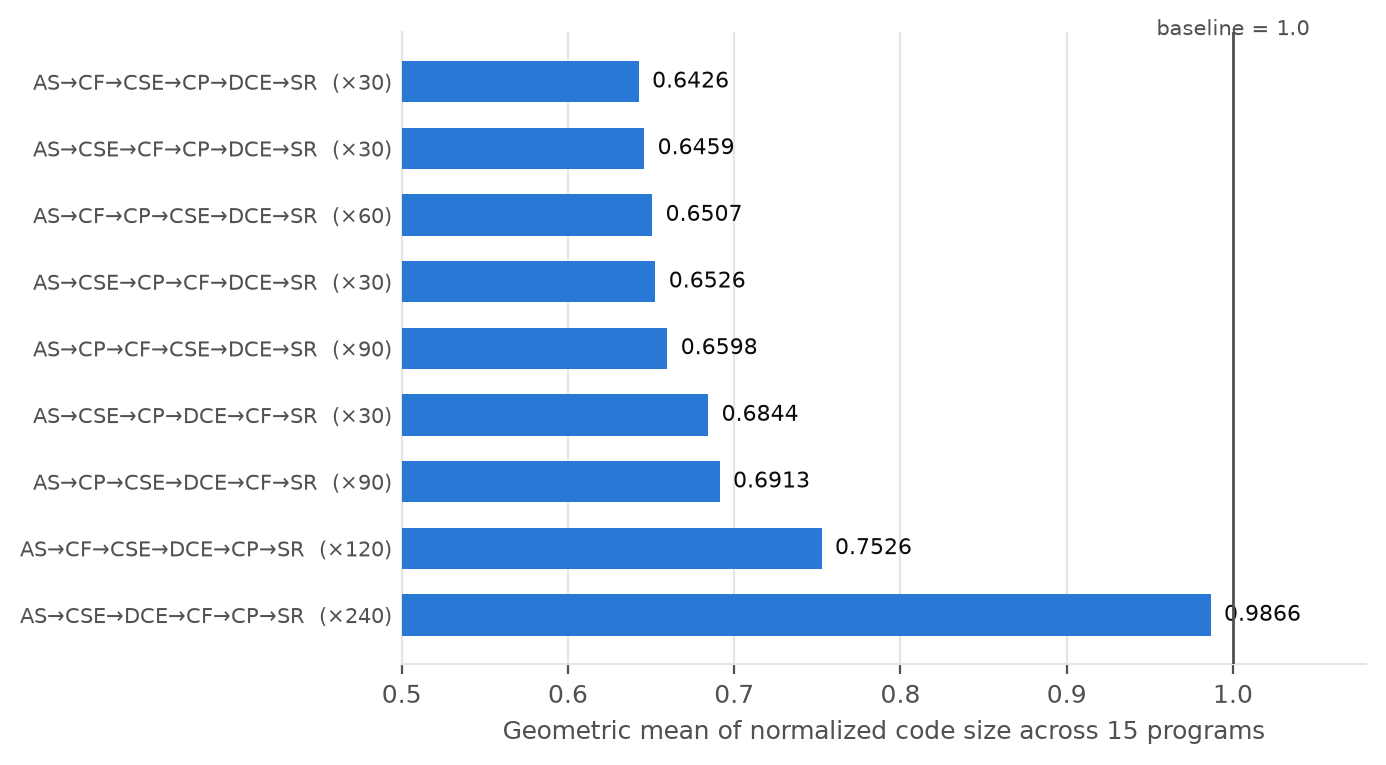
\includegraphics[width=0.95\textwidth]{fig_geomean_classes}
\caption[Geometric-mean normalized code size of the nine ordering classes.]{Geometric-mean normalized code size of the nine ordering classes, each labelled with one representative ordering and the number of orderings in the class. A third of all orderings (240) fall in the worst class and reduce code size by only 1.3\%.}
\label{fig:geomean-classes}
\end{figure}

The table reads as a set of rules. \textbf{Rule 1: DCE must come after CF and CP.} The eight relative orders in which DCE precedes both constant folding and copy propagation form class 9, a third of the whole space, with a size ratio of 0.9866: on thirteen of the fifteen programs these orderings leave the code completely unchanged, and the 1.3\% they do achieve comes entirely from the dead code planted in \code{factorial} and \code{sha\_mix}. DCE removes only instructions whose results are unread, and in the baseline IR every temporary is read at least once; it is constant folding and copy propagation that make temporaries unread, and DCE cannot benefit from what has not yet happened. \textbf{Rule 2: DCE after CF but before CP (class 8) loses a third of the benefit}, because copy propagation is what makes named-variable copies such as \code{sum1 = t18} unread, and without a later DCE those copies survive. \textbf{Rule 3: CF before CP is better than CP before CF} (class 1 against class 5, class 3 against class 5): constant folding substitutes constants through single-assignment variables in a fixed-point loop, whereas copy propagation only substitutes within a basic block, so running CF first exposes more. \textbf{Rule 4: CSE between CF and CP is best} (class 1 against classes 2, 3, and 4), for two reasons. CSE keys its table on the literal operand text, so it finds more matches after CF has replaced temporaries by literals; and CSE replaces a recomputation by a COPY, which only shrinks the code if CP subsequently propagates the copy and DCE deletes it. In class 3, where CP runs before CSE, the copies CSE creates are never propagated and CSE contributes nothing to size. \textbf{Rule 5: SR and AS are size-neutral.} Neither ever changes the instruction count; they only rewrite an instruction in place. Their position affects the cycle estimate alone, which is why the cycle ratio is a range within each class.

\subsubsection*{Structure of the ordering space}

\fig{fig:distinct} shows, per program, how many distinct (size, cycles, dynamic count) outcomes the 720 orderings produce and how many orderings reach the best size. The number of distinct outcomes ranges from 3 (\code{bitcount}, \code{collatz}, \code{gcd}, \code{power}, \code{sha\_mix}) to 23 (\code{2mm}); even for the largest program, 97\% of the orderings duplicate the outcome of some other ordering. The array kernels have more distinct outcomes because the order of SR relative to CF changes the number of multiplications that can be rewritten as additions, which changes the cycle estimate without changing the size.

\begin{figure}[!htb]
\centering
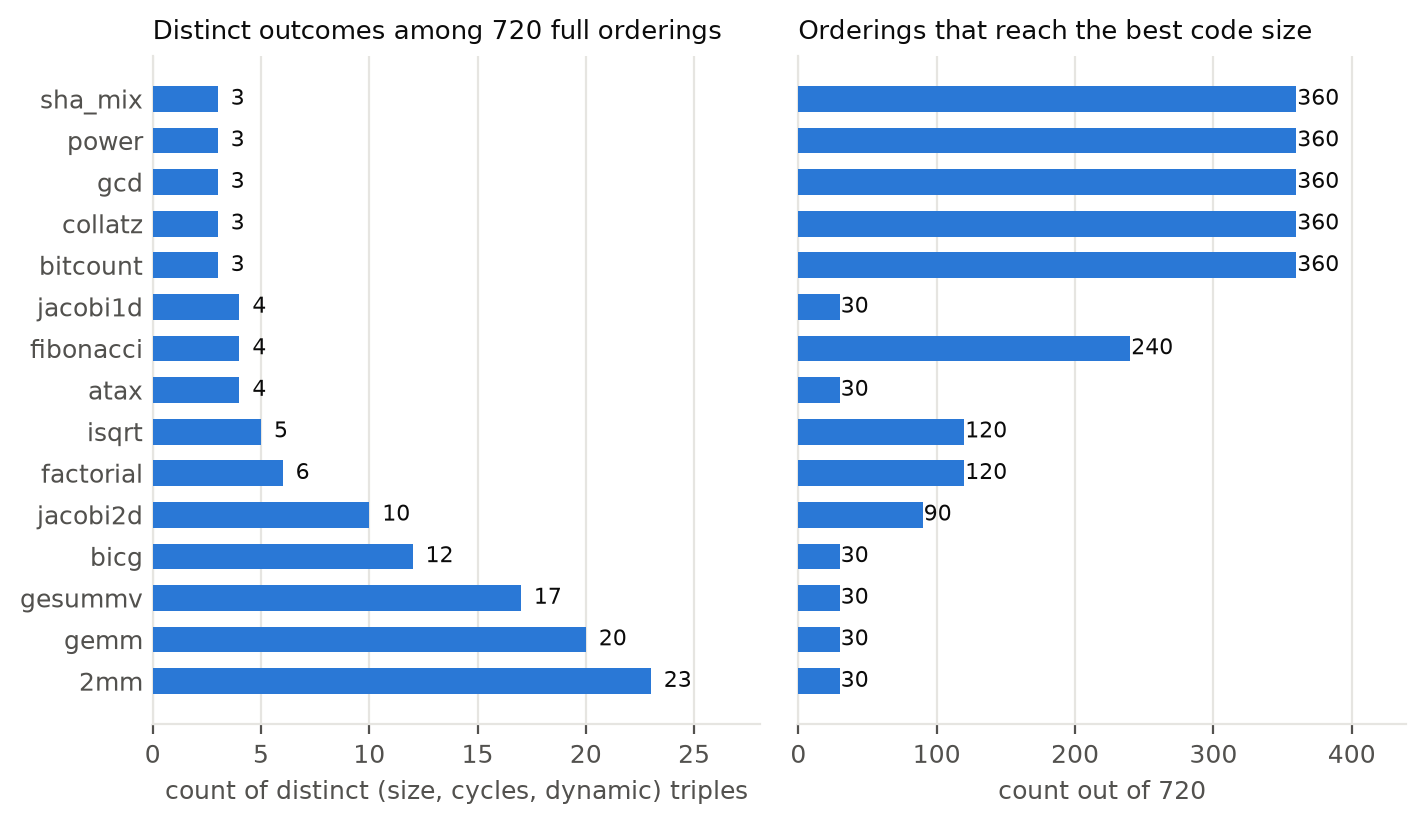
\includegraphics[width=\textwidth]{fig_distinct_outcomes}
\caption[Redundancy of the ordering space per program.]{Redundancy of the ordering space. Left: the number of distinct outcomes among the 720 full orderings; right: the number of orderings that reach the best code size. For the six most array-intensive kernels only one relative order of the four size-relevant passes, 30 orderings, reaches the optimum; for the simplest scalar kernels half of all orderings do.}
\label{fig:distinct}
\end{figure}

The right-hand panel exposes a practical consequence. On the simple scalar programs, 360 of 720 orderings, every ordering in which DCE follows both CF and CP, reach the best size; a compiler writer choosing an order by intuition would have an even chance of being optimal. On the six most array-intensive kernels, only 30 orderings, exactly the class-1 relative order, reach the optimum, and a randomly chosen ordering has a one-in-24 chance. The harder the program, the more precisely the passes must be sequenced.

\fig{fig:position} quantifies the same structure as a marginal effect: the mean normalized code size over all orderings in which a given pass runs first, against those in which it runs last. Moving DCE from first to last improves the mean ratio from 0.988 to 0.659; moving CP from last to first improves it from 0.873 to 0.681; CF from 0.841 to 0.707. CSE's position barely matters (0.789 against 0.793), and SR and AS have no effect at all.


\begin{figure}[!htb]
\centering
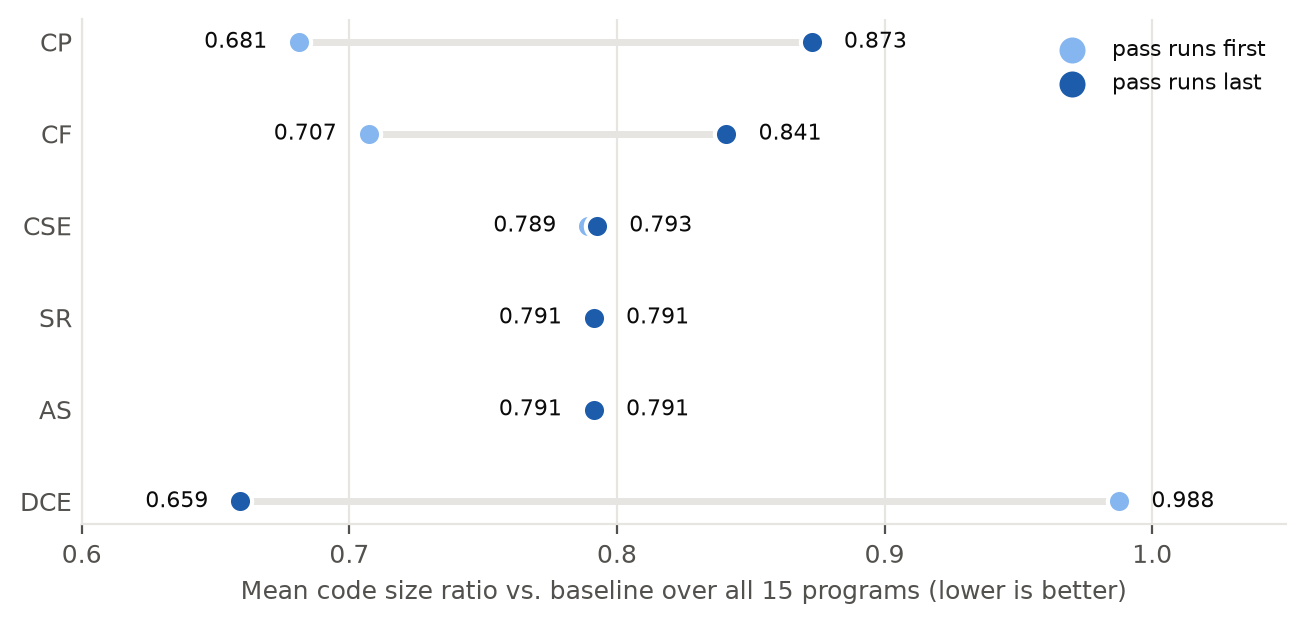
\includegraphics[width=0.92\textwidth]{fig_position_effect}
\caption[Marginal effect of each pass's position on code size.]{Marginal effect of each pass's position. Each row compares the mean normalized code size of the 120 orderings in which the pass runs first (light) with the 120 in which it runs last (dark). DCE is the only pass that should run late; CF and CP should run early; SR and AS do not affect size.}
\label{fig:position}
\end{figure}

\subsubsection*{Pairwise pass interactions}

Table~\ref{tab:interaction} shows the pairwise interaction matrix for \code{gemm}, computed by the visualizer as the mean code size of orderings with pass $A$ before pass $B$ minus that of orderings with $B$ before $A$; \fig{fig:interaction-heatmap} is the corresponding heatmap. A negative entry means $A$ should precede $B$.

\begin{table}[!htb]
\centering\small
\caption{Pairwise interaction matrix for \code{gemm}: mean code size with row pass before column pass minus the reverse (instructions)}
\label{tab:interaction}
\begin{tabular}{L{1.6cm} C{1.4cm} C{1.4cm} C{1.4cm} C{1.4cm} C{1.4cm} C{1.4cm}}
\toprule
\textbf{A $\downarrow$ before B $\rightarrow$} & \textbf{AS} & \textbf{CF} & \textbf{CP} & \textbf{CSE} & \textbf{DCE} & \textbf{SR}\\
\midrule
AS  & 0 & $+$8.1 & $+$6.0 & $+$0.4 & $-$14.4 & 0\\
CF  & $-$8.1 & 0 & $-$2.1 & $-$7.8 & $-$30.4 & $-$8.1\\
CP  & $-$6.0 & $+$2.1 & 0 & $-$5.3 & $-$26.8 & $-$6.0\\
CSE & $-$0.4 & $+$7.8 & $+$5.3 & 0 & $-$14.8 & $-$0.4\\
DCE & $+$14.4 & $+$30.4 & $+$26.8 & $+$14.8 & 0 & $+$14.4\\
SR  & 0 & $+$8.1 & $+$6.0 & $+$0.4 & $-$14.4 & 0\\
\bottomrule
\end{tabular}
\end{table}

\begin{figure}[!htb]
\centering
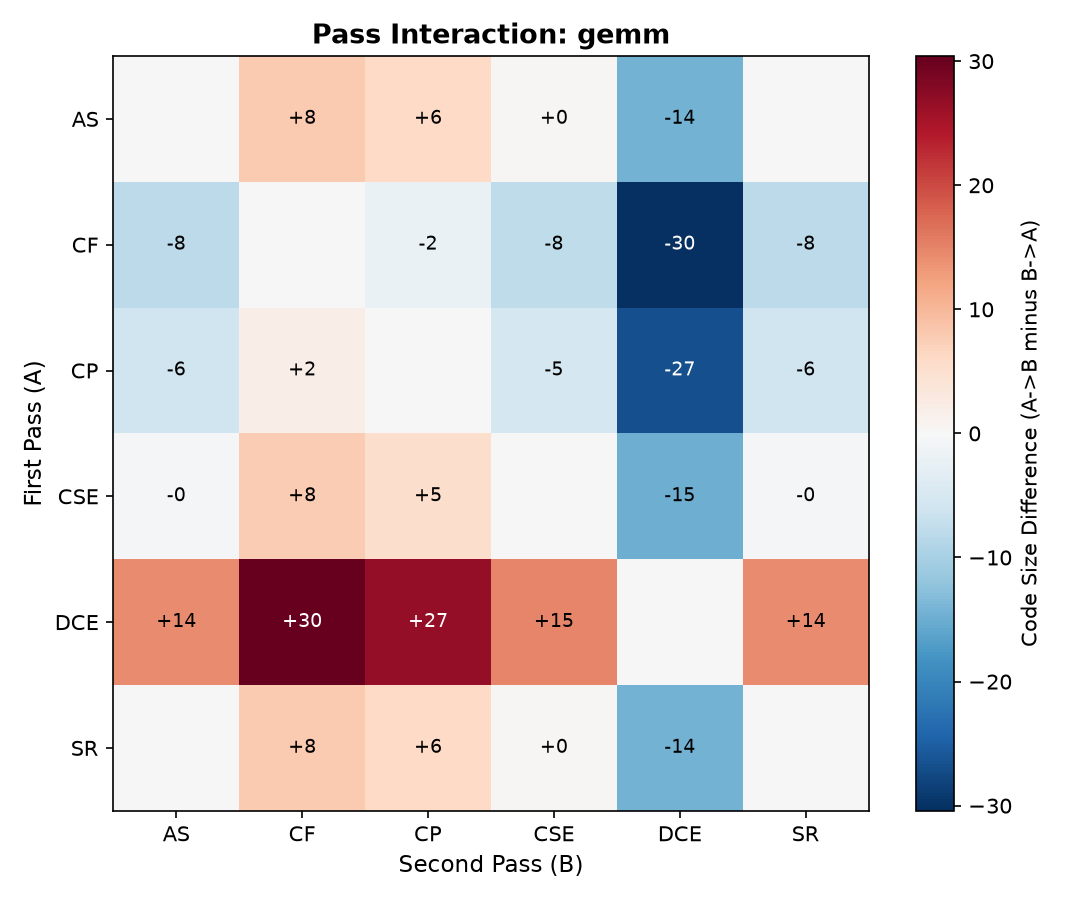
\includegraphics[width=0.55\textwidth]{gemm_pass_interaction}
\caption[Pass interaction heatmap for \code{gemm}.]{Pass interaction heatmap for \code{gemm} produced by the visualizer. Blue cells (negative) indicate that the row pass should run before the column pass; the CF and CP rows against the DCE column carry the largest effects.}
\label{fig:interaction-heatmap}
\end{figure}

The matrix confirms the rules with the direction and magnitude of each pair. Placing CF before DCE saves 30 instructions on average out of 164; CP before DCE saves 27; CSE before DCE saves 15; CF before CP saves 2. The matrix also illustrates a subtlety of marginal analysis. The AS and SR rows are identical and non-zero, even though neither pass ever changes the instruction count. Their entries are not causal: because the matrix averages over all orderings, ``AS before CF'' is correlated with ``DCE relatively later'' in the population of orderings, and the entry reflects the DCE effect rather than any effect of AS. The equivalence-class analysis above, which controls for the other passes, is the correct tool for attribution; the marginal matrix is the right tool for a quick view of which pairs matter most.

\subsubsection*{Where the reduction happens}

\fig{fig:stage-trace} follows the code size of \code{factorial} through each stage of three orderings. Under the best ordering the size stays at 40 through CF, CSE, and CP and drops to 16 at DCE. The enabling passes do not remove a single instruction; they replace instructions with equivalents (a folded expression becomes a LOAD\_CONST, a recomputation becomes a COPY, an operand is renamed) that leave other instructions unread. All of the visible reduction is booked by DCE, but almost none of it is DCE's own doing: run first, DCE removes only the seven planted dead instructions and the ordering ends at 33. Running DCE in the middle, after CF but before CSE and CP, ends at 21. The stage view makes the enabling and consuming roles of the passes visible in a way that final numbers alone cannot; the Optimization Lab page presents exactly this view for any program and ordering.

\begin{figure}[!htb]
\centering
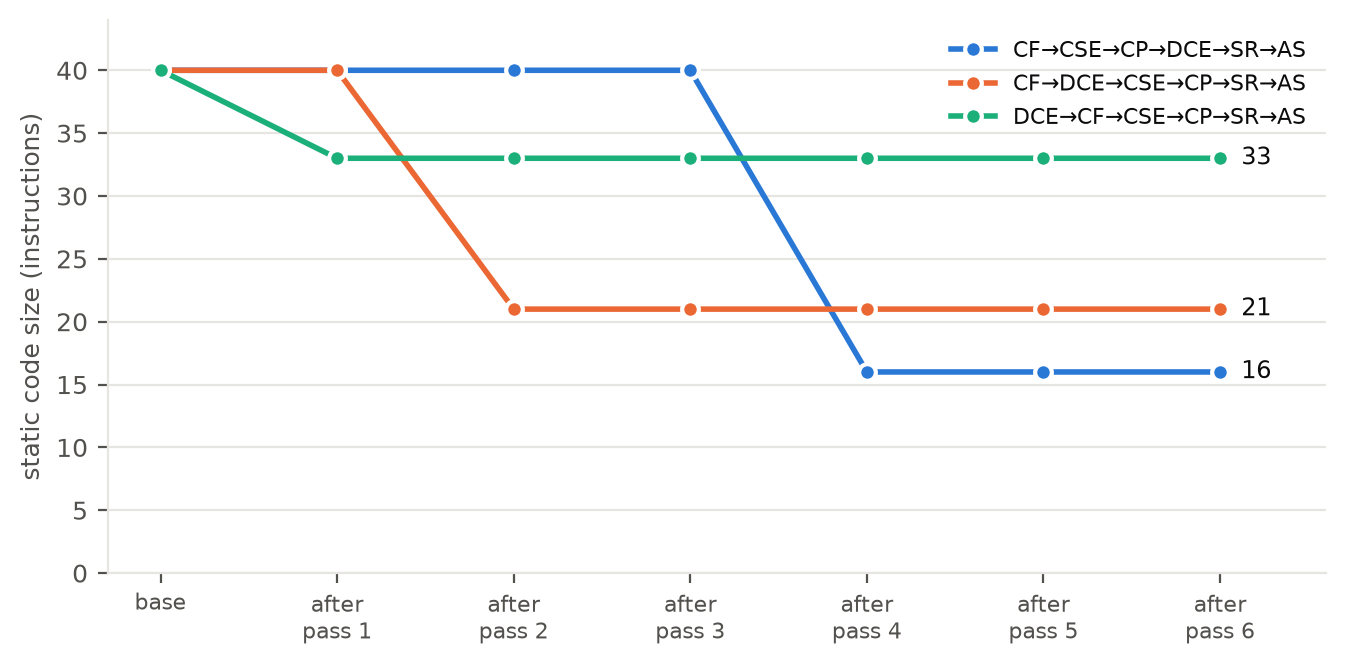
\includegraphics[width=0.9\textwidth]{fig_stage_trace_factorial}
\caption[Code size after each stage of three orderings on \code{factorial}.]{Code size of \code{factorial} after each stage of three orderings. Under the best ordering nothing shrinks until DCE runs; under a DCE-first ordering, DCE removes only the planted dead code and the enabling passes that follow find no consumer for what they expose.}
\label{fig:stage-trace}
\end{figure}

\subsubsection*{Trade-off between code size and estimated cycles}

\fig{fig:pareto} plots every distinct outcome for \code{gemm} in the size-against-cycles plane with the Pareto front drawn by the visualizer. Across all fifteen programs, the two metrics are strongly correlated across orderings: the class with the smallest code is also the class with the lowest cycle estimate and the lowest dynamic count, so in this study there is no trade-off to resolve at the level of classes. There is a residual trade-off within a class, visible as the cycle range in Table~\ref{tab:classes}. It is caused by strength reduction: SR rewrites \code{x * 2} as \code{x + x} (three cycles to one) only when the literal 2 is written in the instruction, and after IR generation the literal sits in a temporary (\code{t4 = 2; t5 = x * t4}). Only constant folding puts the literal into the multiplication, so SR must run after CF to see it. In class 1, orderings with SR after CF have a geometric-mean cycle ratio of 0.7950 and orderings with SR before CF have 0.7999. The Pareto front on \code{gemm} therefore contains points that differ only in cycles, and the front is short: the single best point dominates every other class.

\begin{figure}[!htb]
\centering
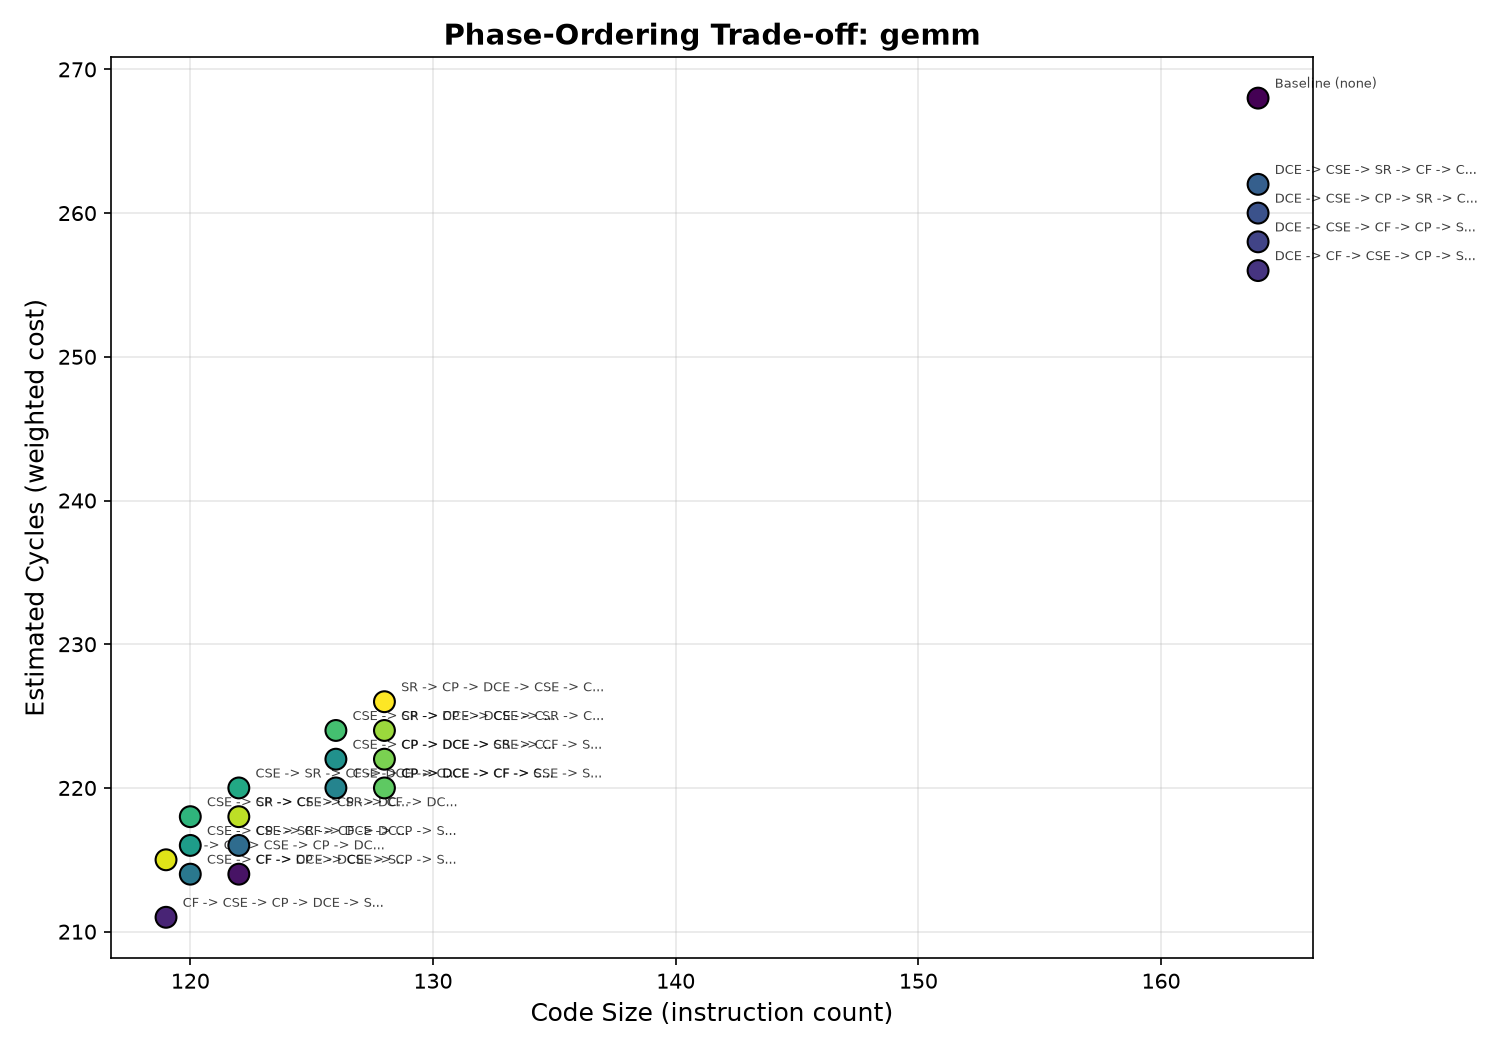
\includegraphics[width=0.78\textwidth]{gemm_tradeoff_scatter}
\caption[Size against estimated cycles for every distinct outcome on \code{gemm}.]{Static code size against estimated cycles for every distinct outcome of the 721 orderings on \code{gemm}, with the Pareto front. Twenty distinct outcomes exist; the best-size class is also the best-cycle class.}
\label{fig:pareto}
\end{figure}


\subsubsection*{Limits of block-local optimization}

The benchmark also quantifies what the block-local passes cannot do. In the optimized \code{factorial} (Appendix~C), the loop body still contains \code{t3 = result * i; result = t3} and \code{t5 = i + 1; i = t5}: the copies into \code{result} and \code{i} survive because both variables are assigned on every iteration, so they fail the single-assignment test for constant propagation, and copy propagation resets at the loop label so it cannot carry \code{t3} into the next iteration's use of \code{result}. A global analysis over a control-flow graph, or an SSA-based representation, would remove these two copies and one comparison temporary in every loop of every benchmark. The array kernels are affected most, since almost all of their instructions live in loop bodies. The measured reductions are therefore a lower bound on what the six transformations could achieve if implemented globally, and the phase-ordering structure found here would need to be re-examined in that setting.

\subsubsection*{Correctness and validation through the RISC-V back end}

Every one of the 10{,}815 optimized programs produced by the exhaustive benchmark printed exactly the same output as its unoptimized baseline, and every one terminated. This is asserted by the benchmark driver and independently by the test suite, which compiles every benchmark under every ordering and compares outputs. It is the strongest available evidence that the six passes are correct in every position, and it is what allows the results above to be interpreted as optimization rather than as accidental deletion.

Table~\ref{tab:asm} carries the size result through code generation. For each benchmark, the baseline IR and the class-1 optimized IR were lowered to RV32IM assembly, and the assembly instructions were counted, excluding labels, directives, and the constant runtime print routine. The reductions in assembly instruction count range from 13.5\% (\code{bicg}) to 50.4\% (\code{factorial}), with a geometric mean of 26.0\% against 35.7\% at the IR level. The assembly reduction is smaller than the IR reduction because the stack-slot back end spends several instructions on every IR instruction that touches memory, and those loads and stores dilute the effect; a register allocator would bring the two figures closer. The test suite verifies that, for all fifteen benchmarks, the assembly produced from the optimized IR prints the same values in the RV32IM simulator as the interpreter produces from the same IR, and returns the same exit status.

\begin{table}[!htb]
\centering\small
\caption{Static size at the IR level and at the RV32IM assembly level, baseline versus best ordering}
\label{tab:asm}
\begin{tabular}{L{1.8cm} C{1.5cm} C{1.5cm} C{1.6cm} C{1.6cm} C{1.6cm} C{1.9cm}}
\toprule
 & \multicolumn{2}{c}{\textbf{IR instructions}} & \multicolumn{3}{c}{\textbf{RV32IM instructions}} & \\
\cmidrule(lr){2-3}\cmidrule(lr){4-6}
\textbf{Program} & base & best & base & best & red.\ \% & \textbf{Simulator}\\
\midrule
2mm & 252 & 185 & 775 & 629 & 18.8 & output matches\\
atax & 101 & 78 & 340 & 292 & 14.1 & output matches\\
bicg & 94 & 73 & 342 & 296 & 13.5 & output matches\\
bitcount & 33 & 19 & 102 & 74 & 27.5 & output matches\\
collatz & 42 & 26 & 123 & 91 & 26.0 & output matches\\
factorial & 40 & 16 & 119 & 59 & 50.4 & output matches\\
fibonacci & 22 & 13 & 61 & 43 & 29.5 & output matches\\
gcd & 21 & 14 & 70 & 56 & 20.0 & output matches\\
gemm & 164 & 119 & 507 & 409 & 19.3 & output matches\\
gesummv & 106 & 78 & 385 & 323 & 16.1 & output matches\\
isqrt & 50 & 27 & 140 & 84 & 40.0 & output matches\\
jacobi1d & 76 & 50 & 254 & 191 & 24.8 & output matches\\
jacobi2d & 144 & 95 & 476 & 346 & 27.3 & output matches\\
power & 71 & 47 & 184 & 136 & 26.1 & output matches\\
sha\_mix & 106 & 68 & 290 & 214 & 26.2 & output matches\\
\midrule
\textbf{Geomean ratio} & & \textbf{0.6426} & & & \textbf{0.7402} & \\
\bottomrule
\end{tabular}
\end{table}

\section{Non Functional Requirements Results Achieved}

All eight non-functional requirements were met. Table~\ref{tab:nfr-status} gives the measured evidence for each.

\begin{table}[!htb]
\centering\small
\caption{Non Functional Requirements Status Table}
\label{tab:nfr-status}
\begin{tabular}{L{1.5cm} L{4.6cm} L{1.6cm} L{5.5cm}}
\toprule
\textbf{NFR} & \textbf{Requirement} & \textbf{Status} & \textbf{Measured result}\\
\midrule
NFR-1 & Correctness under every ordering and after lowering & Achieved & 10{,}815 of 10{,}815 optimized programs match baseline output; 15 of 15 benchmarks match in the RV32IM simulator\\
NFR-2 & Determinism and reproducibility & Achieved & Repeated runs and runs on Linux and Windows produce identical IR, assembly, and metric tables; no randomness in any module\\
NFR-3 & Performance: single-program exhaustive benchmark $<$ 10 s; all programs $<$ 60 s & Achieved & Slowest program (\code{2mm}) 5.21 s; fastest (\code{gcd}) 0.17 s; all fifteen programs with plots 23.5 s\\
NFR-4 & Transparency and readability & Achieved & Compiler core about 4{,}000 lines in 19 modules; largest module 560 lines; every module has an algorithm description at its head\\
NFR-5 & Portability and ease of installation & Achieved & Pure Python 3.10+ with five pip dependencies; pre-built front end committed; no database, network, or CDN dependency; verified on Linux and Windows\\
NFR-6 & Usability & Achieved & Keyboard reordering of passes; errors reported with phase, message, line, and column and underlined in the editor; compile and optimize responses well under one second for all benchmarks\\
NFR-7 & Maintainability and test coverage & Achieved & 185 test cases in 3 modules, all passing in 3.98 s; type annotations throughout; tests run before every merge\\
NFR-8 & Extensibility & Achieved & Adding a pass requires one module and one registry entry; verified when CP, SR, and AS were added after CF, DCE, and CSE with no change to the pass manager, benchmark, or API\\
\bottomrule
\end{tabular}
\end{table}

Two of the requirements deserve comment. NFR-3 was set so that the Phase-Ordering Explorer could run the exhaustive benchmark interactively in the browser; the measured 5.2 seconds for the largest program, most of it spent interpreting 721 optimized programs of 4{,}000 to 5{,}000 executed instructions each, leaves comfortable margin, and programs of the size a student would type run in well under a second. NFR-4 is the requirement that distinguishes this project from a study on a production compiler; the line counts per module reported in Chapter 4 are the evidence that it was met, and the fact that every result in this chapter can be traced by hand through the listings in Appendix~C is its practical consequence.

\section{Comparison of Results with Existing Works}

Direct numerical comparison with the literature is limited by two differences. The published studies use production or research compilers with tens to hundreds of passes, so their orderings and ours are not the same objects; and most of them report improvements over an already-optimized baseline such as \code{-O3} or \code{-Oz}, whereas this project reports improvements over unoptimized code, because the unoptimized IR is the only baseline that is independent of any ordering. The comparison in Table~\ref{tab:comparison} is therefore made on the structural findings, which are comparable, and the magnitudes are reported with their baselines stated.

\begin{table}[!htb]
\centering\small
\caption{Comparison of the findings of this project with existing work}
\label{tab:comparison}
\begin{tabular}{L{3.0cm} L{5.0cm} L{5.4cm}}
\toprule
\textbf{Work} & \textbf{Their finding} & \textbf{This project}\\
\midrule
Cooper et al.\ \cite{cooper1999} & Genetic search over 10 passes finds program-specific sequences that produce smaller code than the fixed default. & Exhaustive search over 6 passes: the best class is the \emph{same} for all 15 programs, so on this pass set a fixed sequence is optimal. Program specificity appears only in how many orderings are optimal (30 to 360 of 720).\\
Kulkarni et al.\ \cite{kulkarni2004,kulkarni2006} & Most phase sequences produce duplicate function instances; dormant phases are common; exhaustive enumeration of distinct instances is feasible. & 720 orderings produce 3 to 23 distinct outcomes per program (0.4\% to 3.2\%); SR and AS are dormant with respect to size on every program; the class structure is fully enumerated.\\
Muchnick \cite{muchnick1997} & Recommends constant folding early and dead code elimination as a late, repeated clean-up. & Quantified: DCE first gives a 1.2\% mean reduction, DCE last gives 34.1\%; CF first 29.3\% versus CF last 15.9\%.\\
Whitfield \& Soffa \cite{whitfield1997} & Transformations have enabling and disabling relationships that depend on the program. & Only enabling relationships were found among these six passes; no pass disables another on any program (no ordering is worse than the baseline).\\
Jain et al.\ \cite{jain2022} & Reinforcement learning improves code size over LLVM \code{-Oz} while holding execution time; size and time can conflict. & Size and both time proxies are minimized by the same class on all 15 programs; the only residual conflict is SR's position relative to CF, worth 0.5\% of cycles.\\
Cummins et al.\ \cite{cummins2023} & A learned model improves LLVM code size by about 3\% over \code{-Oz}. & 35.7\% over \emph{unoptimized} code; not comparable in magnitude, but the same metric (static instruction count) and the same objective.\\
Georgiou et al.\ \cite{georgiou2018} & On Cortex-M targets the default optimization level is often not the best; pass interactions are the cause. & Consistent: on the array kernels only 1 in 24 relative orders is optimal; a default chosen without measurement would be suboptimal 23 times in 24.\\
Click \& Cooper \cite{click1995} & Combining analyses can beat any sequence of separate passes. & The surviving loop-carried copies in every benchmark are exactly the cases a combined or global analysis would remove; identified as future work.\\
\bottomrule
\end{tabular}
\end{table}

The comparison supports three conclusions. First, the qualitative phenomena reported for production compilers, redundancy of the ordering space, dormancy of some passes, and the enabling role of constant propagation, are reproduced exactly, not approximately, on a six-pass infrastructure, which suggests that they are properties of the transformations themselves rather than of any particular compiler. Second, the program-specificity that motivates search and learning methods at production scale does not appear at this scale: with six local passes a single fixed sequence is optimal for every program tested. Program-specific ordering presumably emerges from the interactions of loop and interprocedural transformations that are absent here, and the infrastructure is positioned to test that hypothesis by adding them. Third, the magnitude of the effect, a factor of more than 25 between the best and worst classes in mean code-size reduction, is large enough that the phase-ordering problem deserves the attention it receives in the literature and in the classroom.

\section{Project GUI Snapshots}
\label{sec:gui}

The interactive application is the delivery vehicle for everything in this chapter. It is served by a single Python process and opens to the Playground. Its design uses a dark, editor-like theme with a monospaced face for code and a sans-serif face for controls, a persistent left sidebar for the five sections, and a ``pipeline rail'' at the top of every page that shows which compiler stages the page exercises. All interactions are available from the keyboard. The fifth section, Reference, documents the passes, the cost model, and the language so that the application is self-contained; the four working sections are shown below.

\subsubsection*{1. Playground}

The Playground (\fig{fig:gui-playground}) is the entry point. The user writes a program in the CodeMirror editor or loads one of the fifteen benchmarks from the example picker, which groups them by suite and shows each program's documentation comment as a title with bullet points. Compiling (button or Ctrl+Enter) fills the right-hand panel, whose tabs show the token stream as coloured chips, the syntax tree as a collapsible outline, the symbol table with scope depths and IR names, and the three-address code. When compilation fails, the badge next to the button names the phase and line, and the editor underlines the offending position; \fig{fig:gui-error} shows a semantic error reported for an undeclared variable.

\begin{figure}[!htb]
\centering
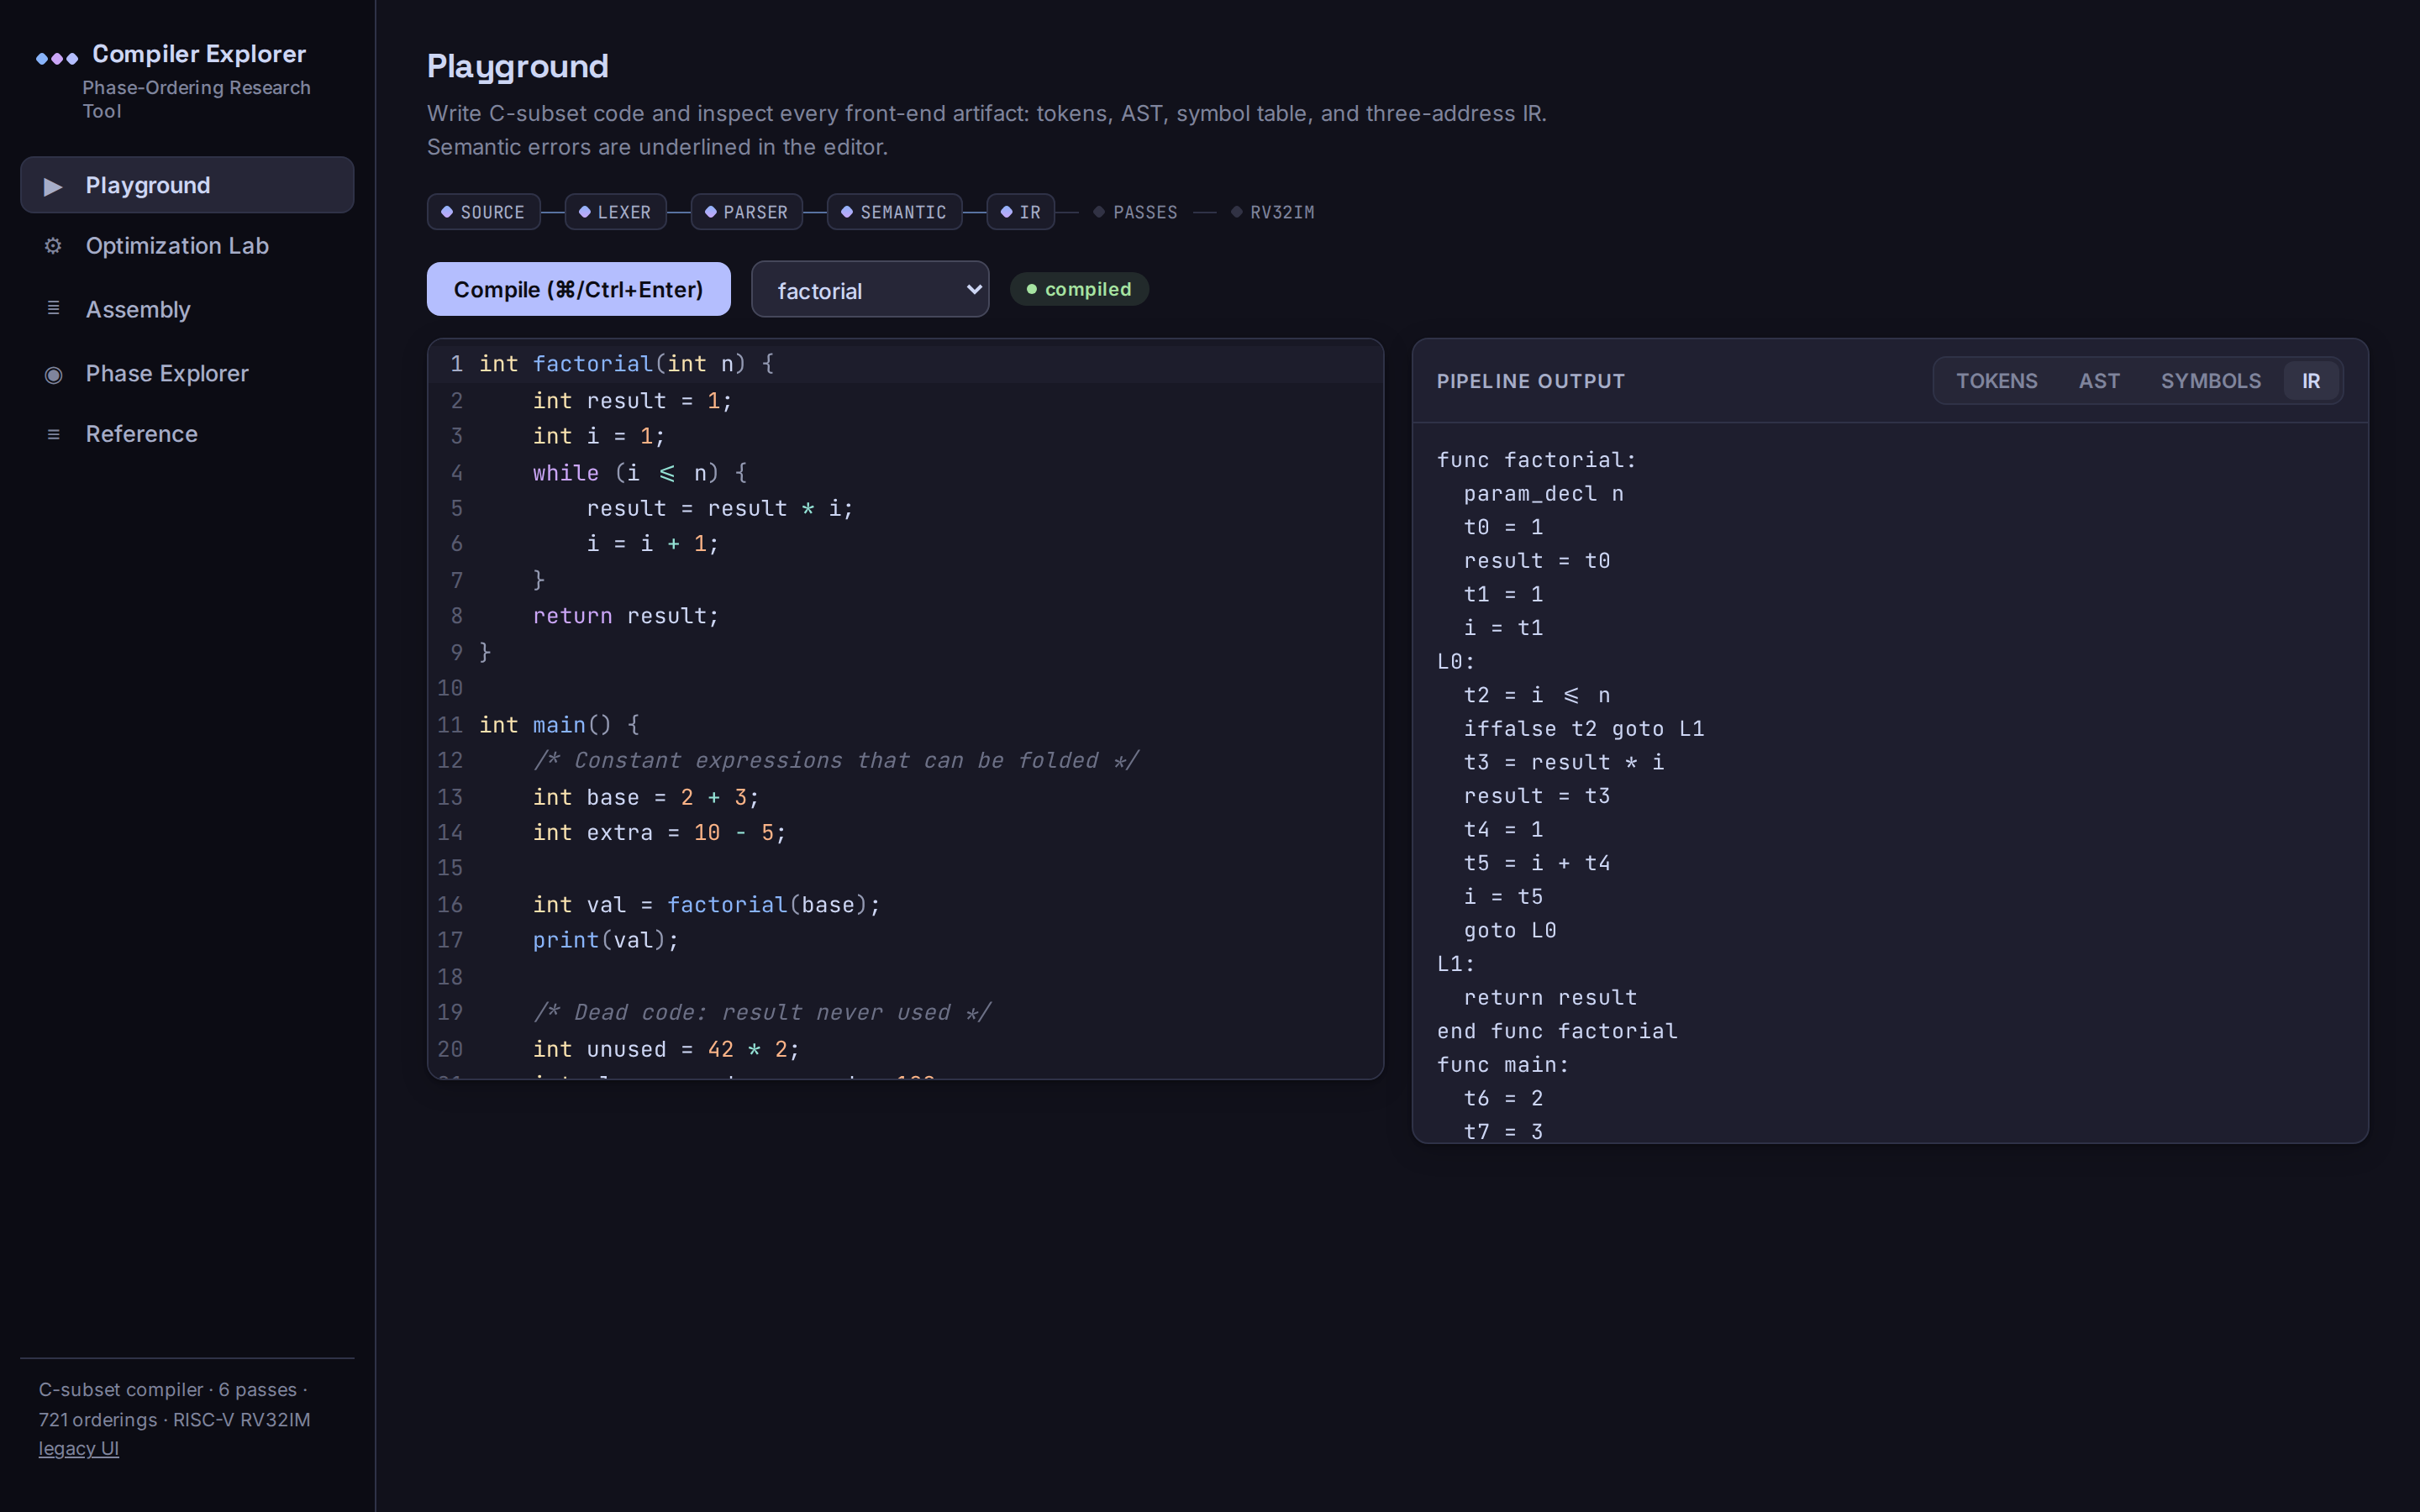
\includegraphics[width=0.82\textwidth]{gui_playground}
\caption[Playground page showing the IR of \code{factorial}.]{Playground page with the \code{factorial} benchmark loaded and compiled; the IR tab shows the three-address code with functions, labels, and temporaries.}
\label{fig:gui-playground}
\end{figure}

\begin{figure}[!htb]
\centering
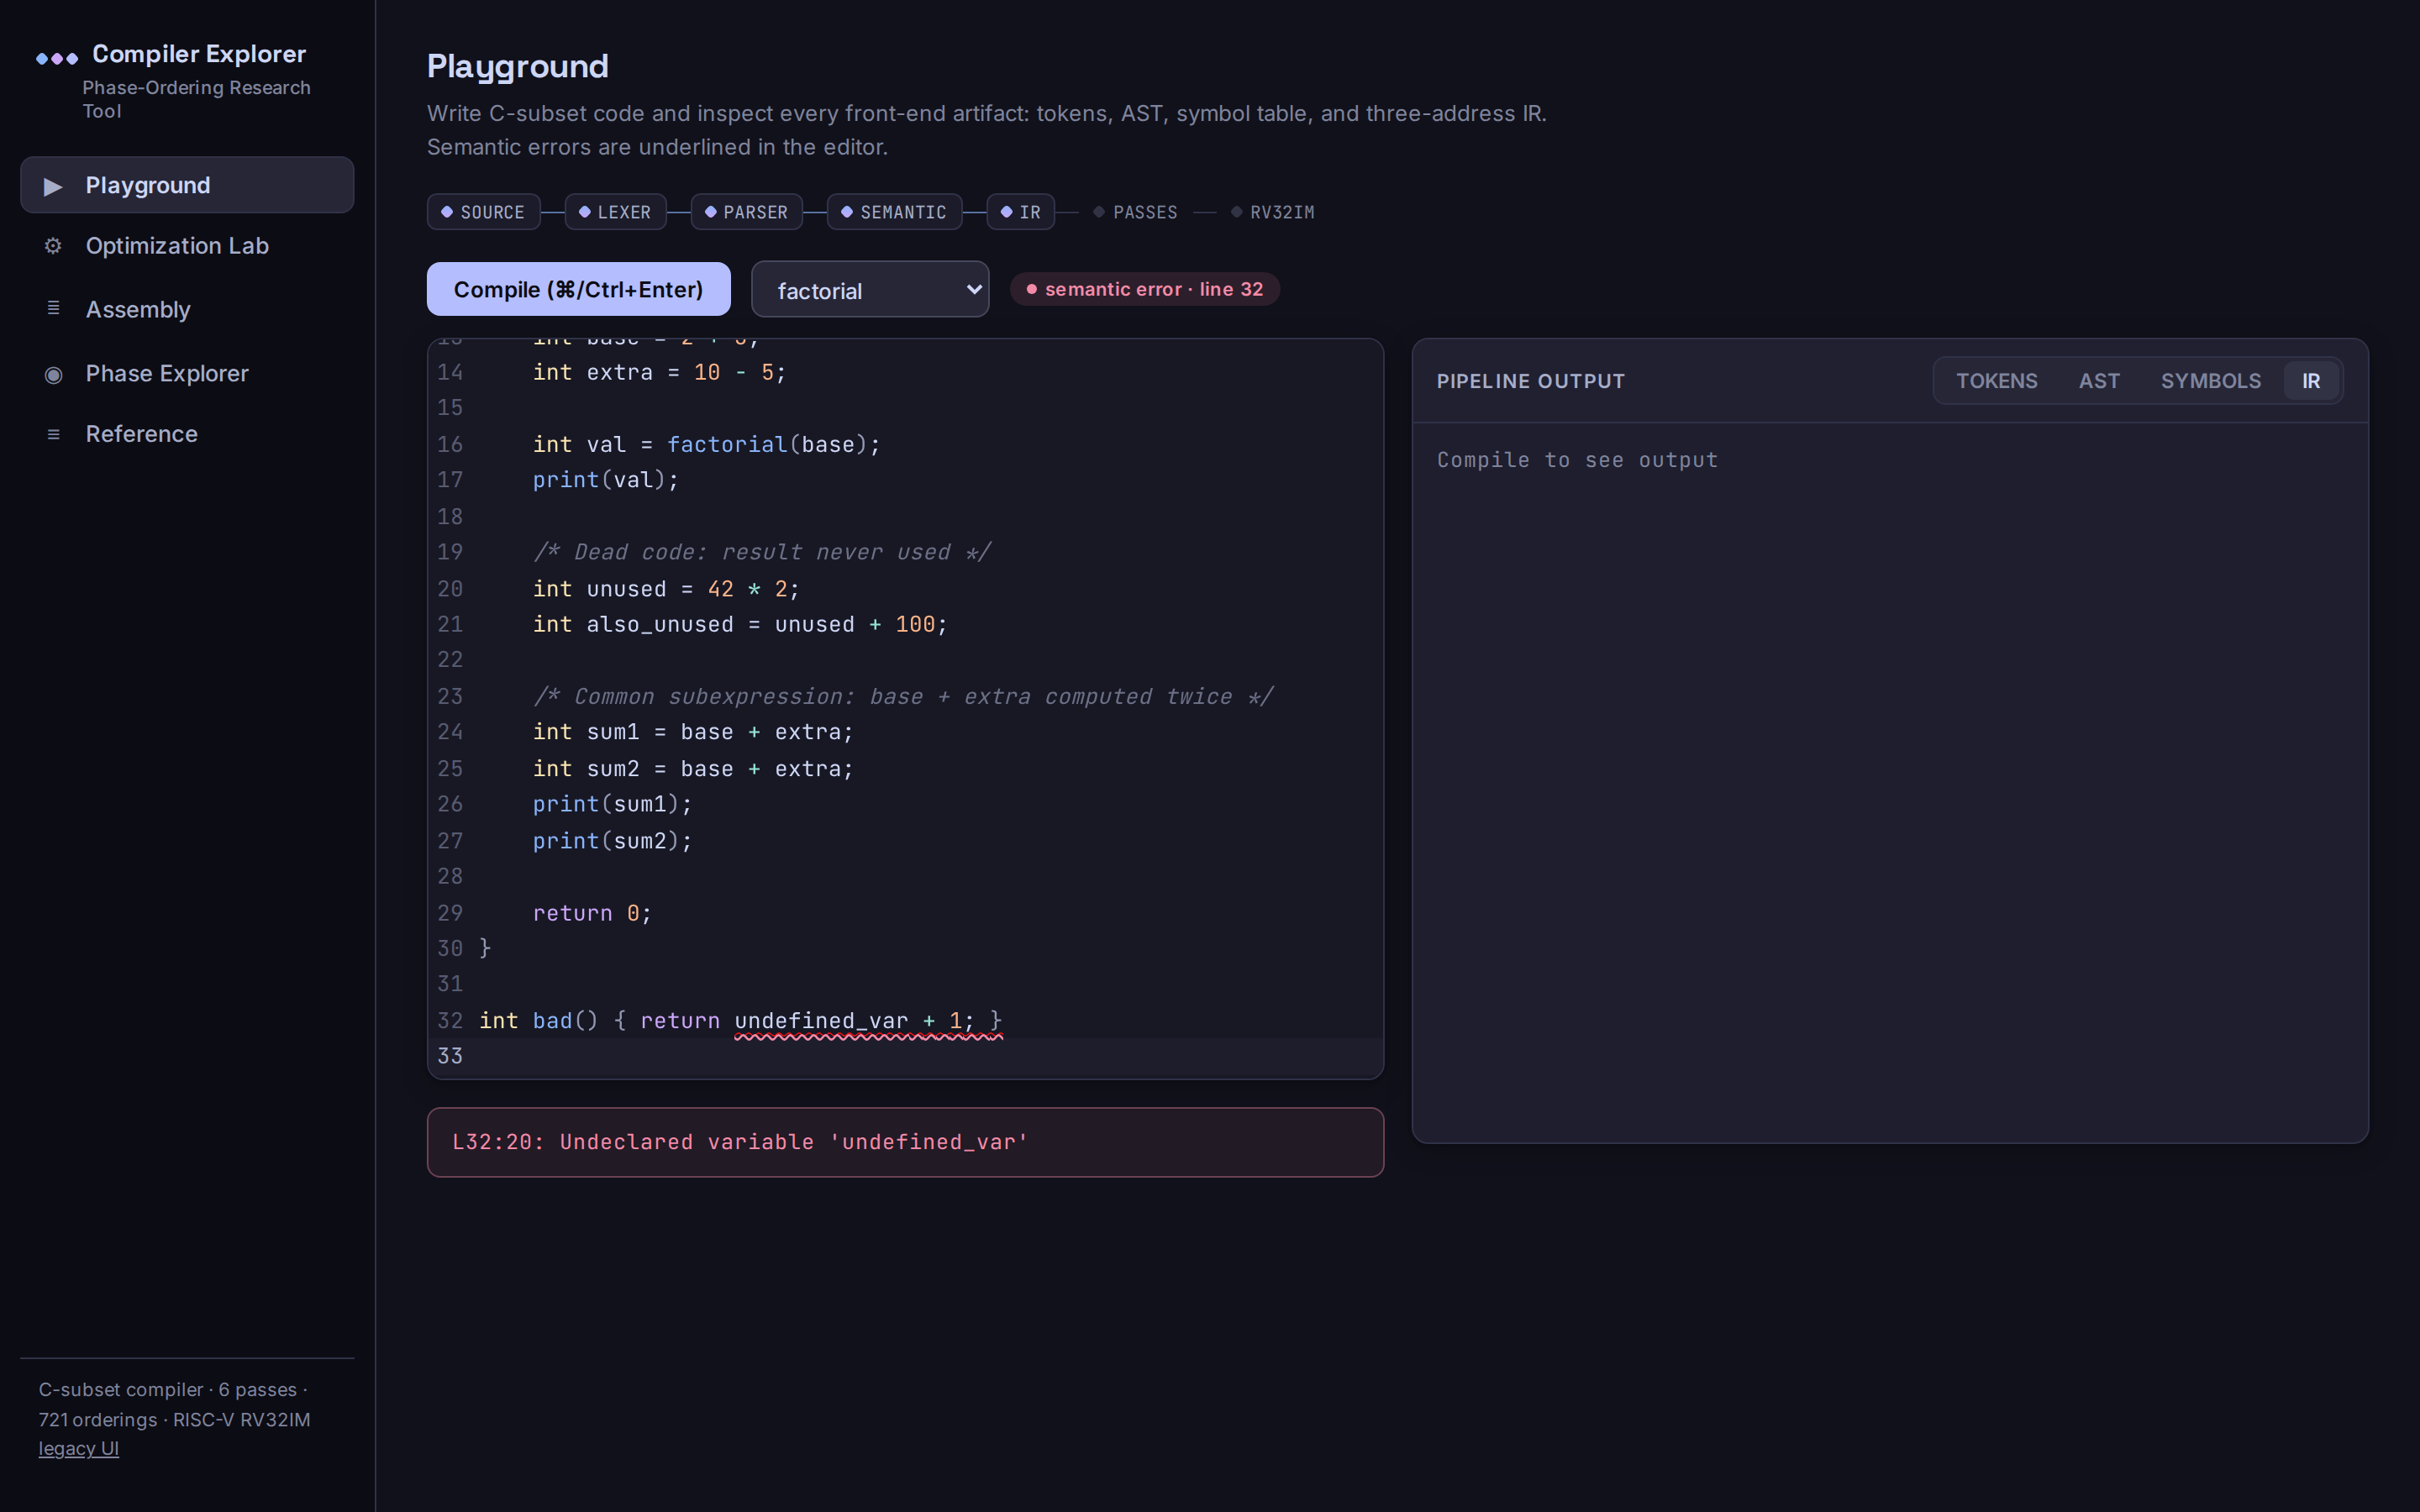
\includegraphics[width=0.82\textwidth]{gui_playground_error}
\caption[Playground page reporting a semantic error.]{Playground page reporting a semantic error. The badge names the phase and line, and the editor underlines the undeclared variable at the reported position.}
\label{fig:gui-error}
\end{figure}

\subsubsection*{2. Optimization Lab}

The Optimization Lab (\fig{fig:gui-optlab}) is the phase-ordering problem made interactive. The six passes appear as numbered chips that can be dragged into any order, or moved with the arrow keys. Running the pipeline produces one card per stage showing the code size after that stage and its delta; selecting a card displays the IR after that stage with lines removed by the pass struck through and lines added highlighted, and the three stat tiles report code size, estimated cycles, and the effect of the selected pass. In the figure, \code{factorial} has been run under the best ordering and the DCE stage is selected, showing the 24 instructions it removed and the strikethrough of the constant-holding temporaries that CF and CP made dead.

\begin{figure}[!htb]
\centering
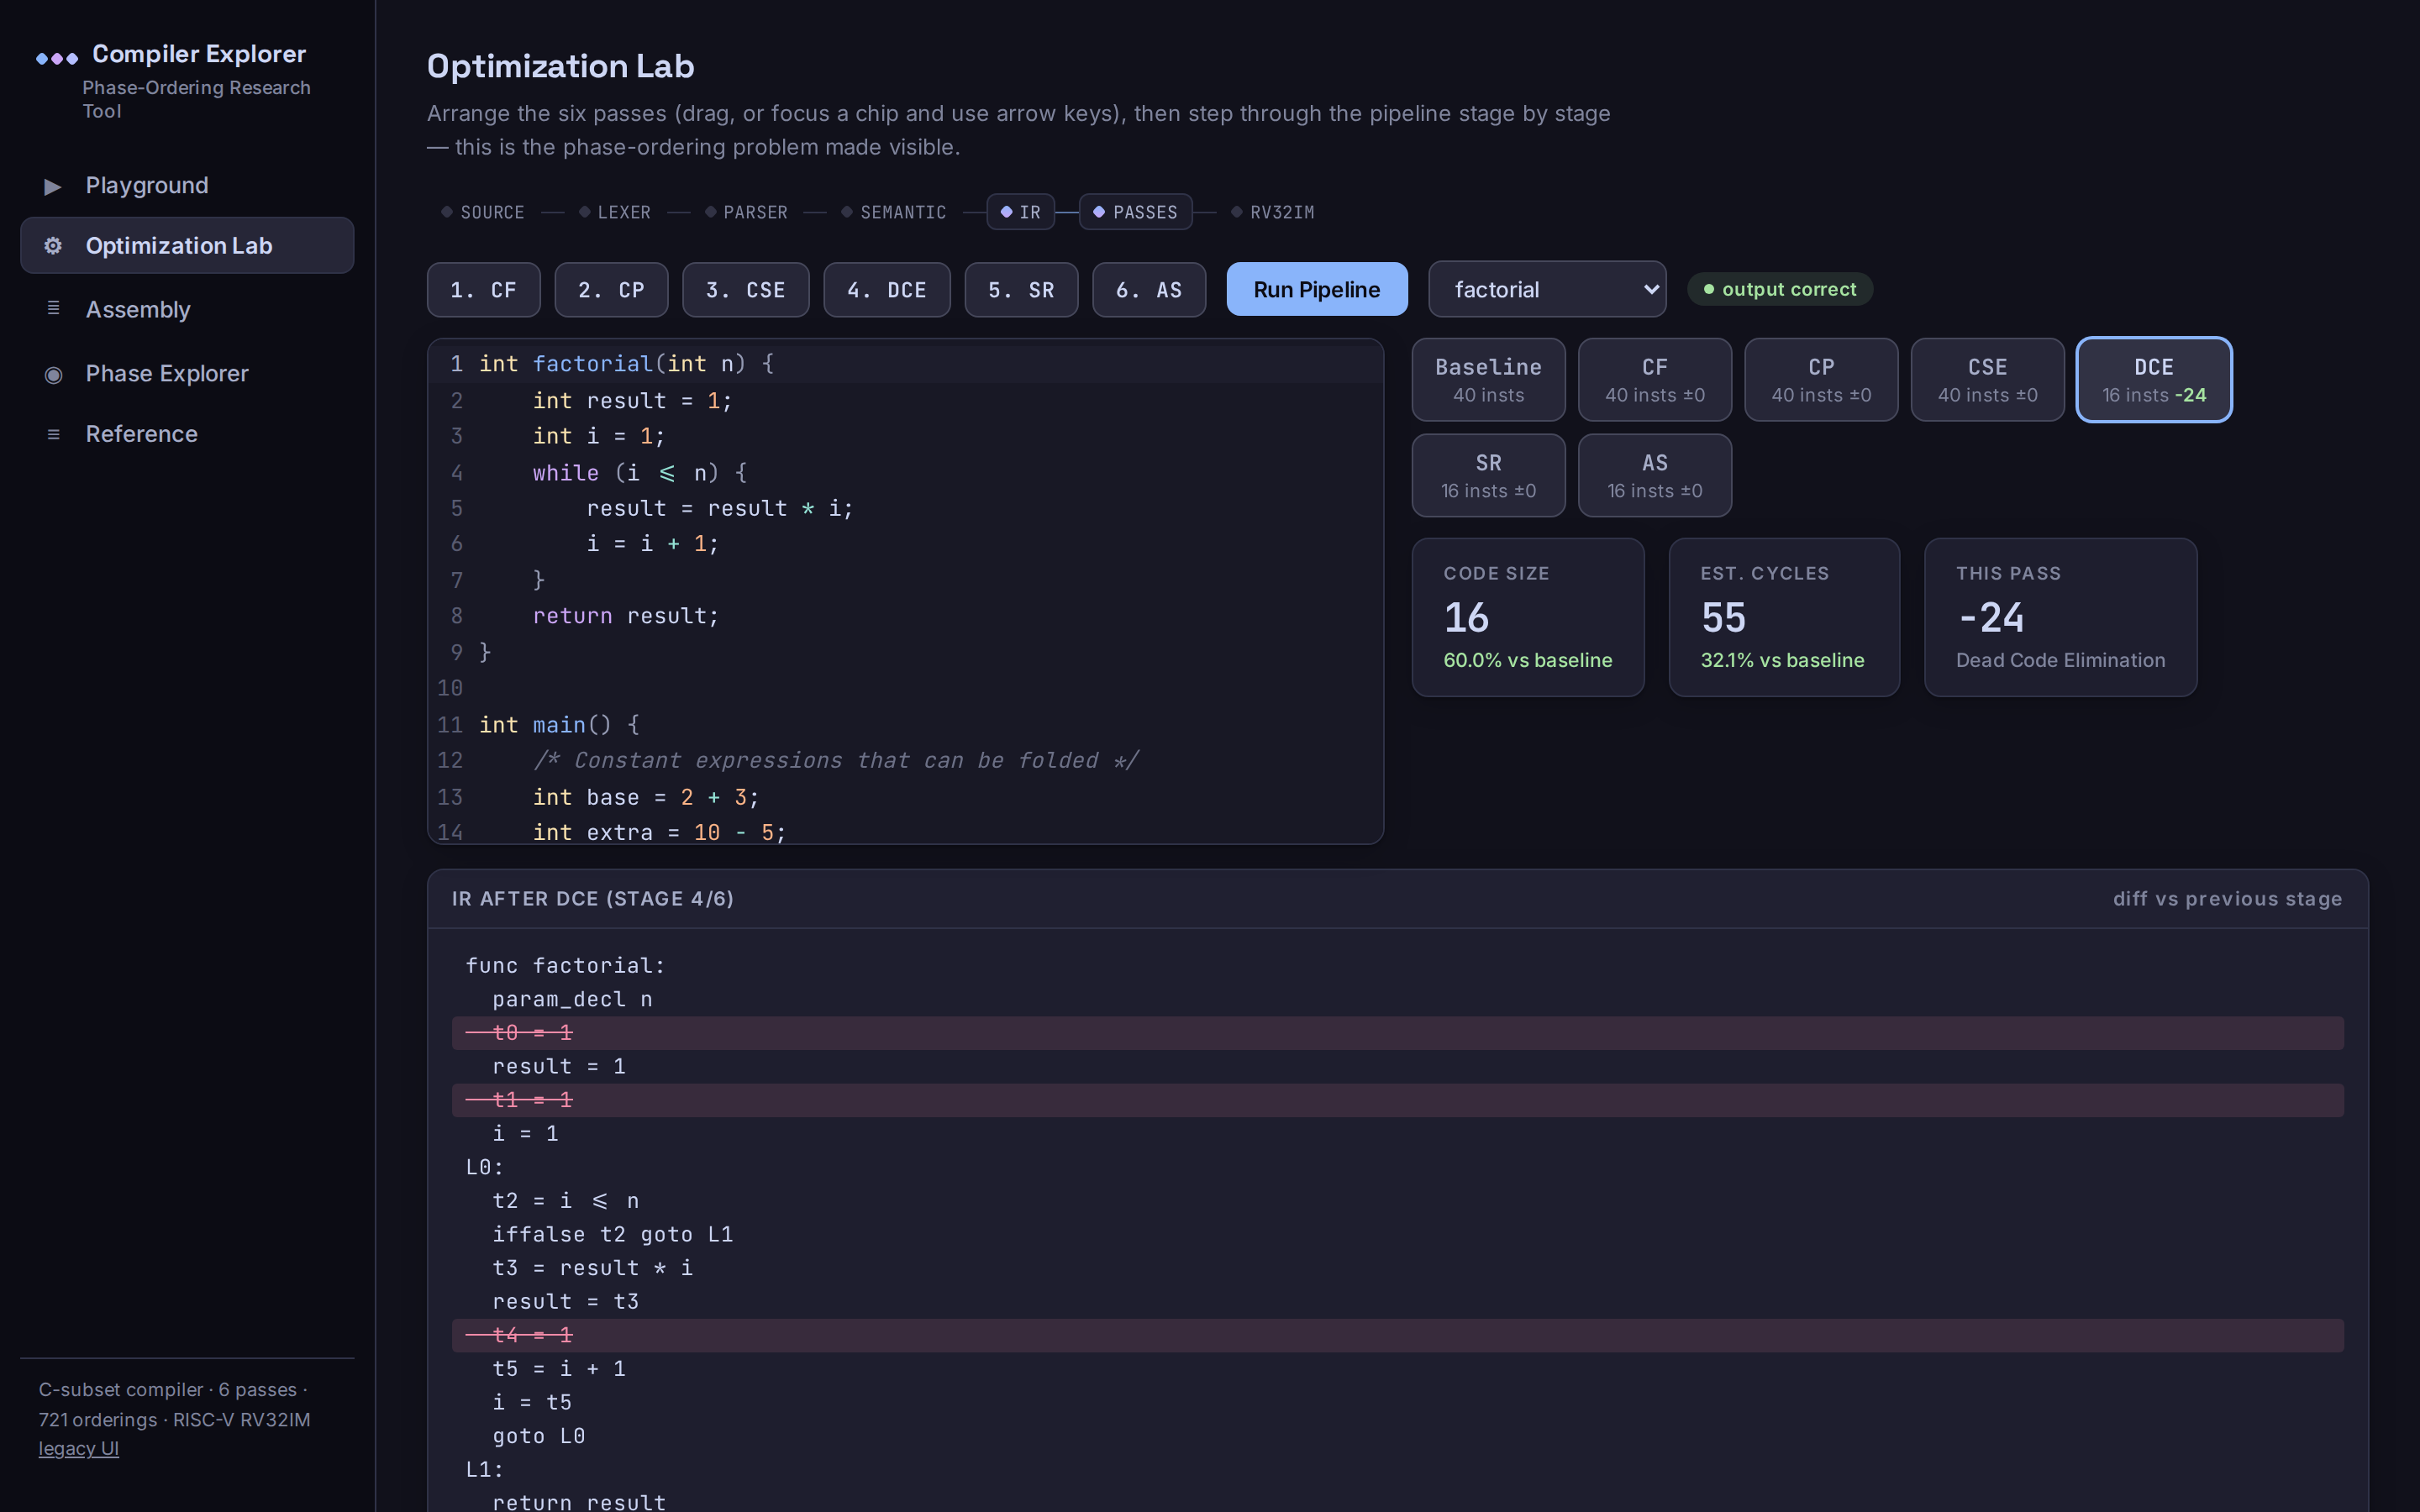
\includegraphics[width=0.82\textwidth]{gui_optlab_diff}
\caption[Optimization Lab page with the DCE stage of the best ordering selected.]{Optimization Lab page: \code{factorial} under CF, CP, CSE, DCE, SR, AS with the DCE stage selected. The stage cards show that no instruction is removed until DCE; the diff view strikes through the 24 instructions DCE removed.}
\label{fig:gui-optlab}
\end{figure}

\subsubsection*{3. Assembly}

The Assembly page (\fig{fig:gui-assembly}) shows the three-address code and the generated RV32IM assembly side by side, with a toggle for optimized or unoptimized input. Hovering over an IR line highlights the assembly lines it produced, using the mapping returned by the assembly endpoint, so that a student can see, for example, that a single \code{t2 = i <= n} becomes two loads, a \code{slt}, an \code{xori}, and a store.

\begin{figure}[!htb]
\centering
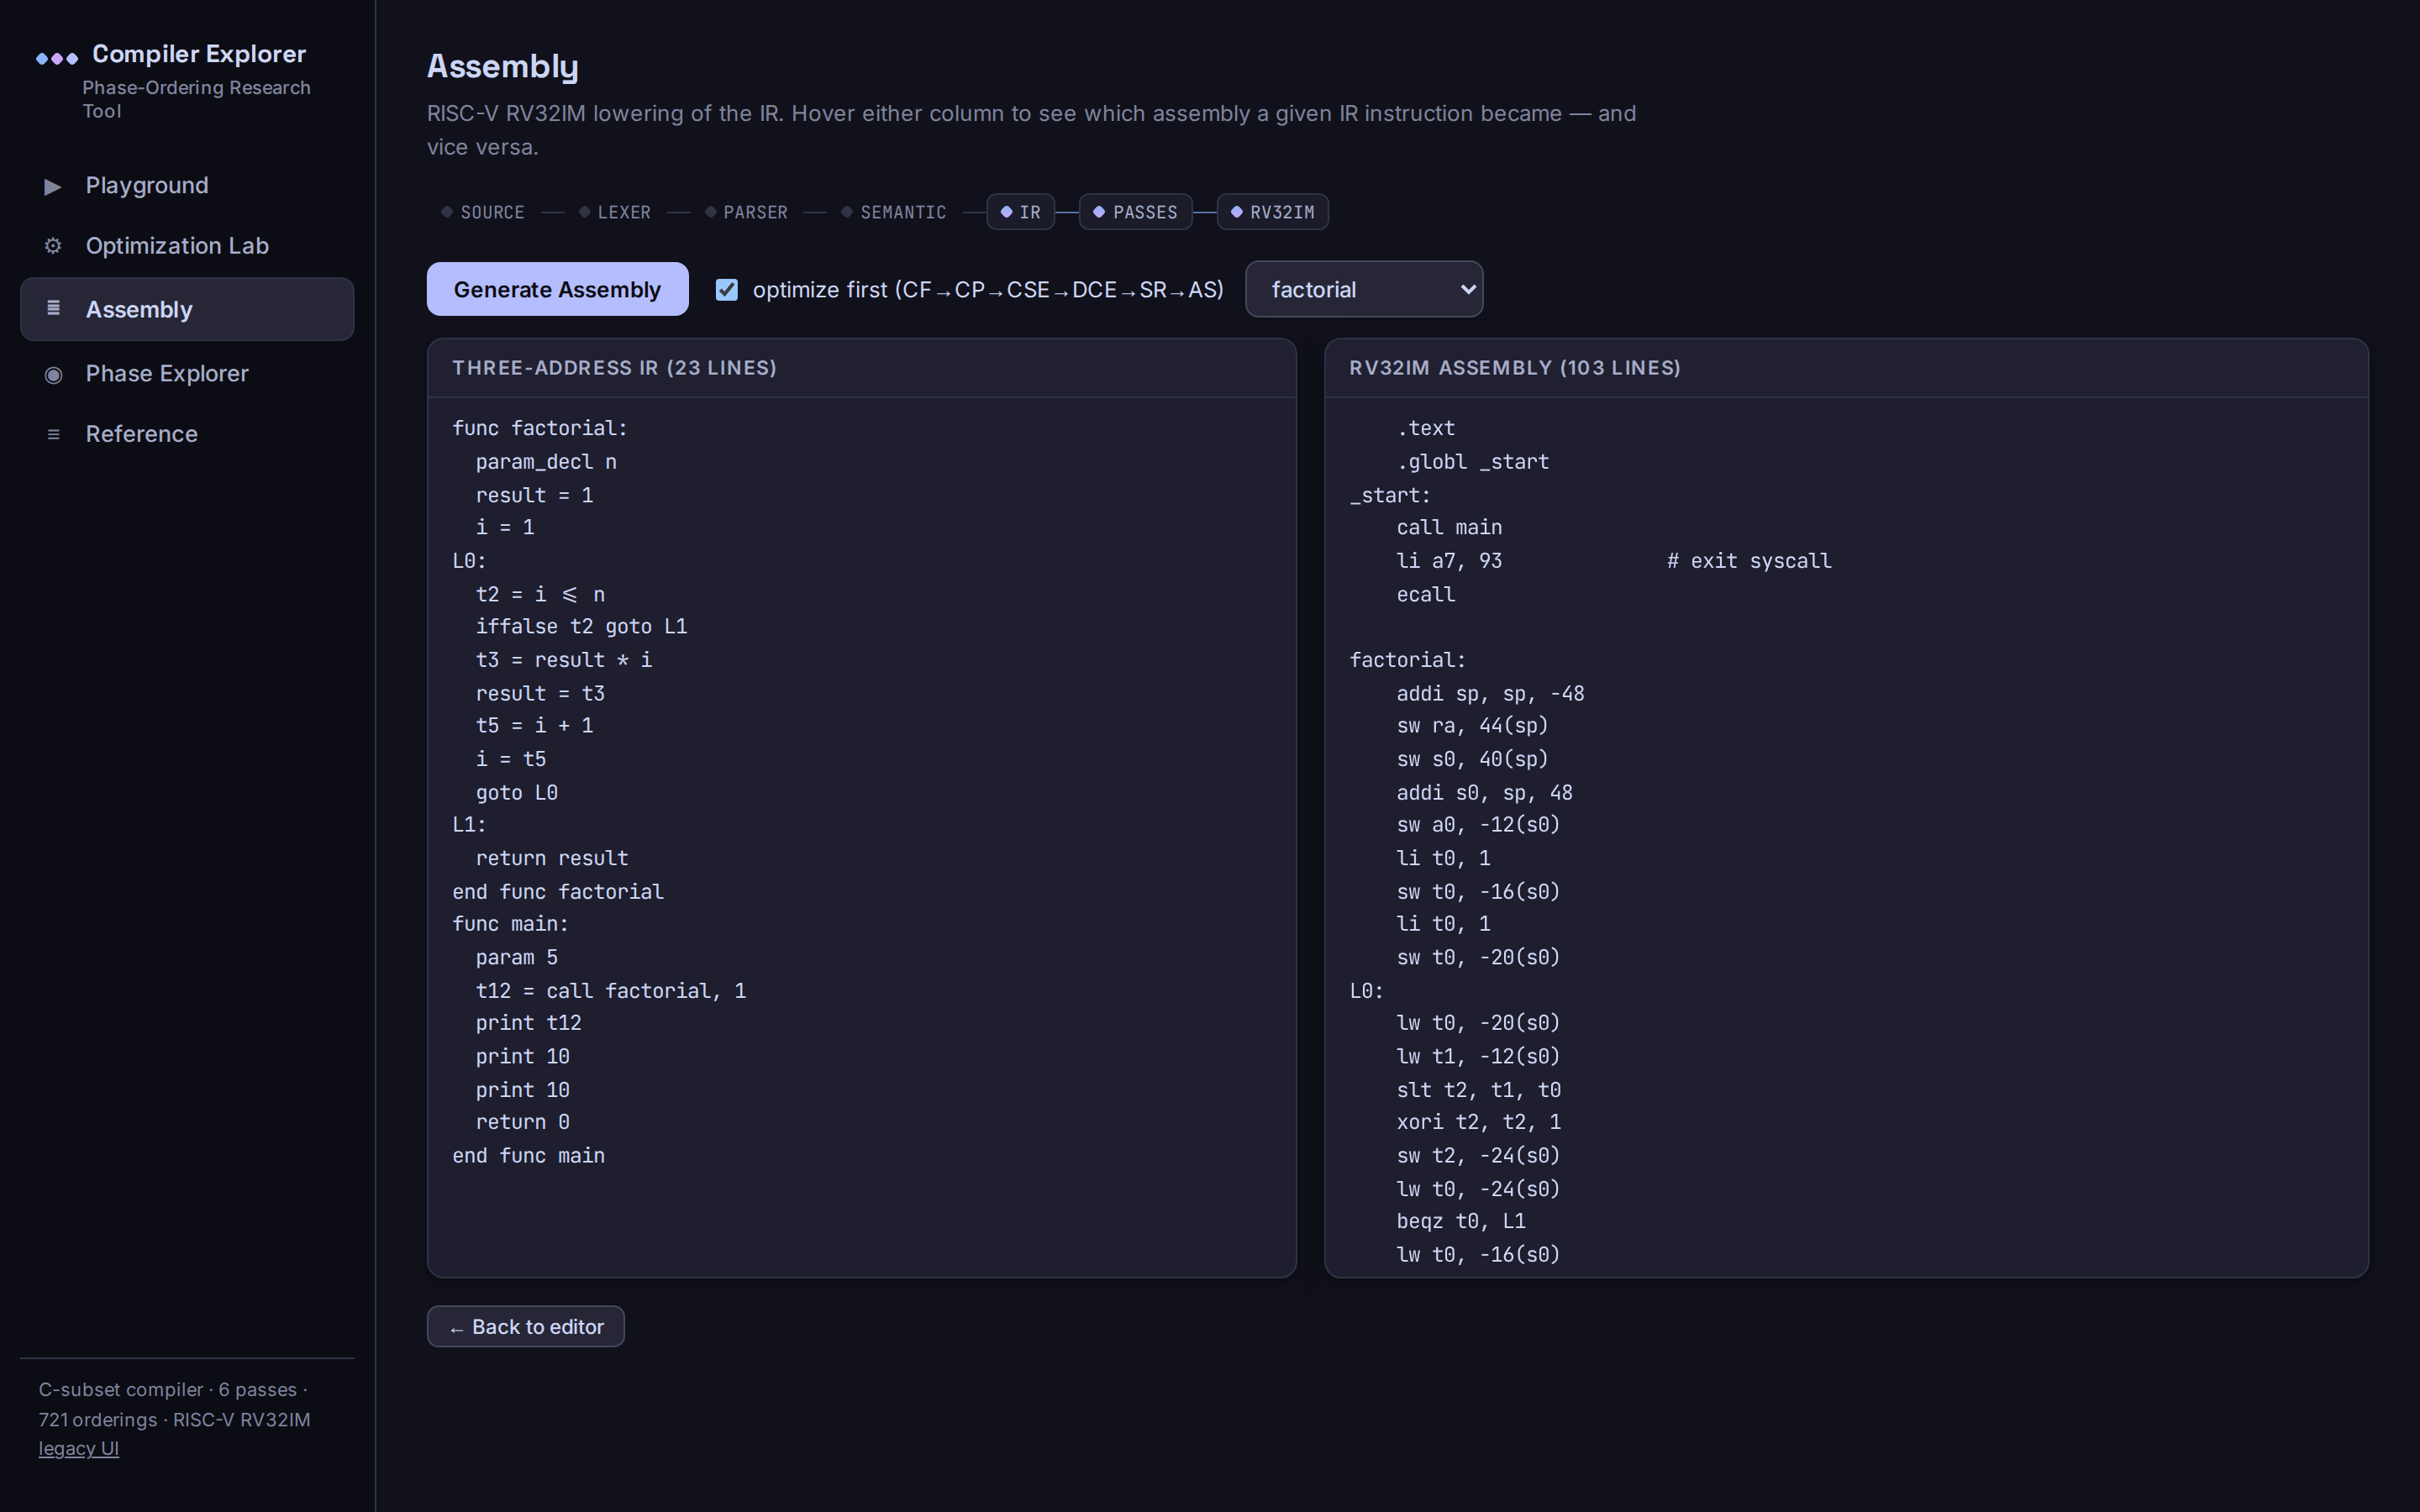
\includegraphics[width=0.82\textwidth]{gui_assembly}
\caption[Assembly page with hover-linked IR and RV32IM assembly.]{Assembly page for \code{factorial}: optimized IR on the left, RV32IM assembly on the right, with hover linking between corresponding lines.}
\label{fig:gui-assembly}
\end{figure}

\subsubsection*{4. Phase-Ordering Explorer}

The Phase-Ordering Explorer (\fig{fig:gui-explorer}) runs all 721 orderings on the current program in the server and plots the results in the browser: a scatter of static code size against estimated cycles with the Pareto-optimal orderings highlighted, and a bar chart of the ten smallest results. Clicking a point reveals its ordering and metrics. The badges report how many orderings are Pareto-optimal and confirm that every ordering's output was verified against the baseline. In the figure, \code{gemm} shows twenty distinct outcomes spread from 119 to 164 instructions, with the best class at the lower left.

\begin{figure}[!htb]
\centering
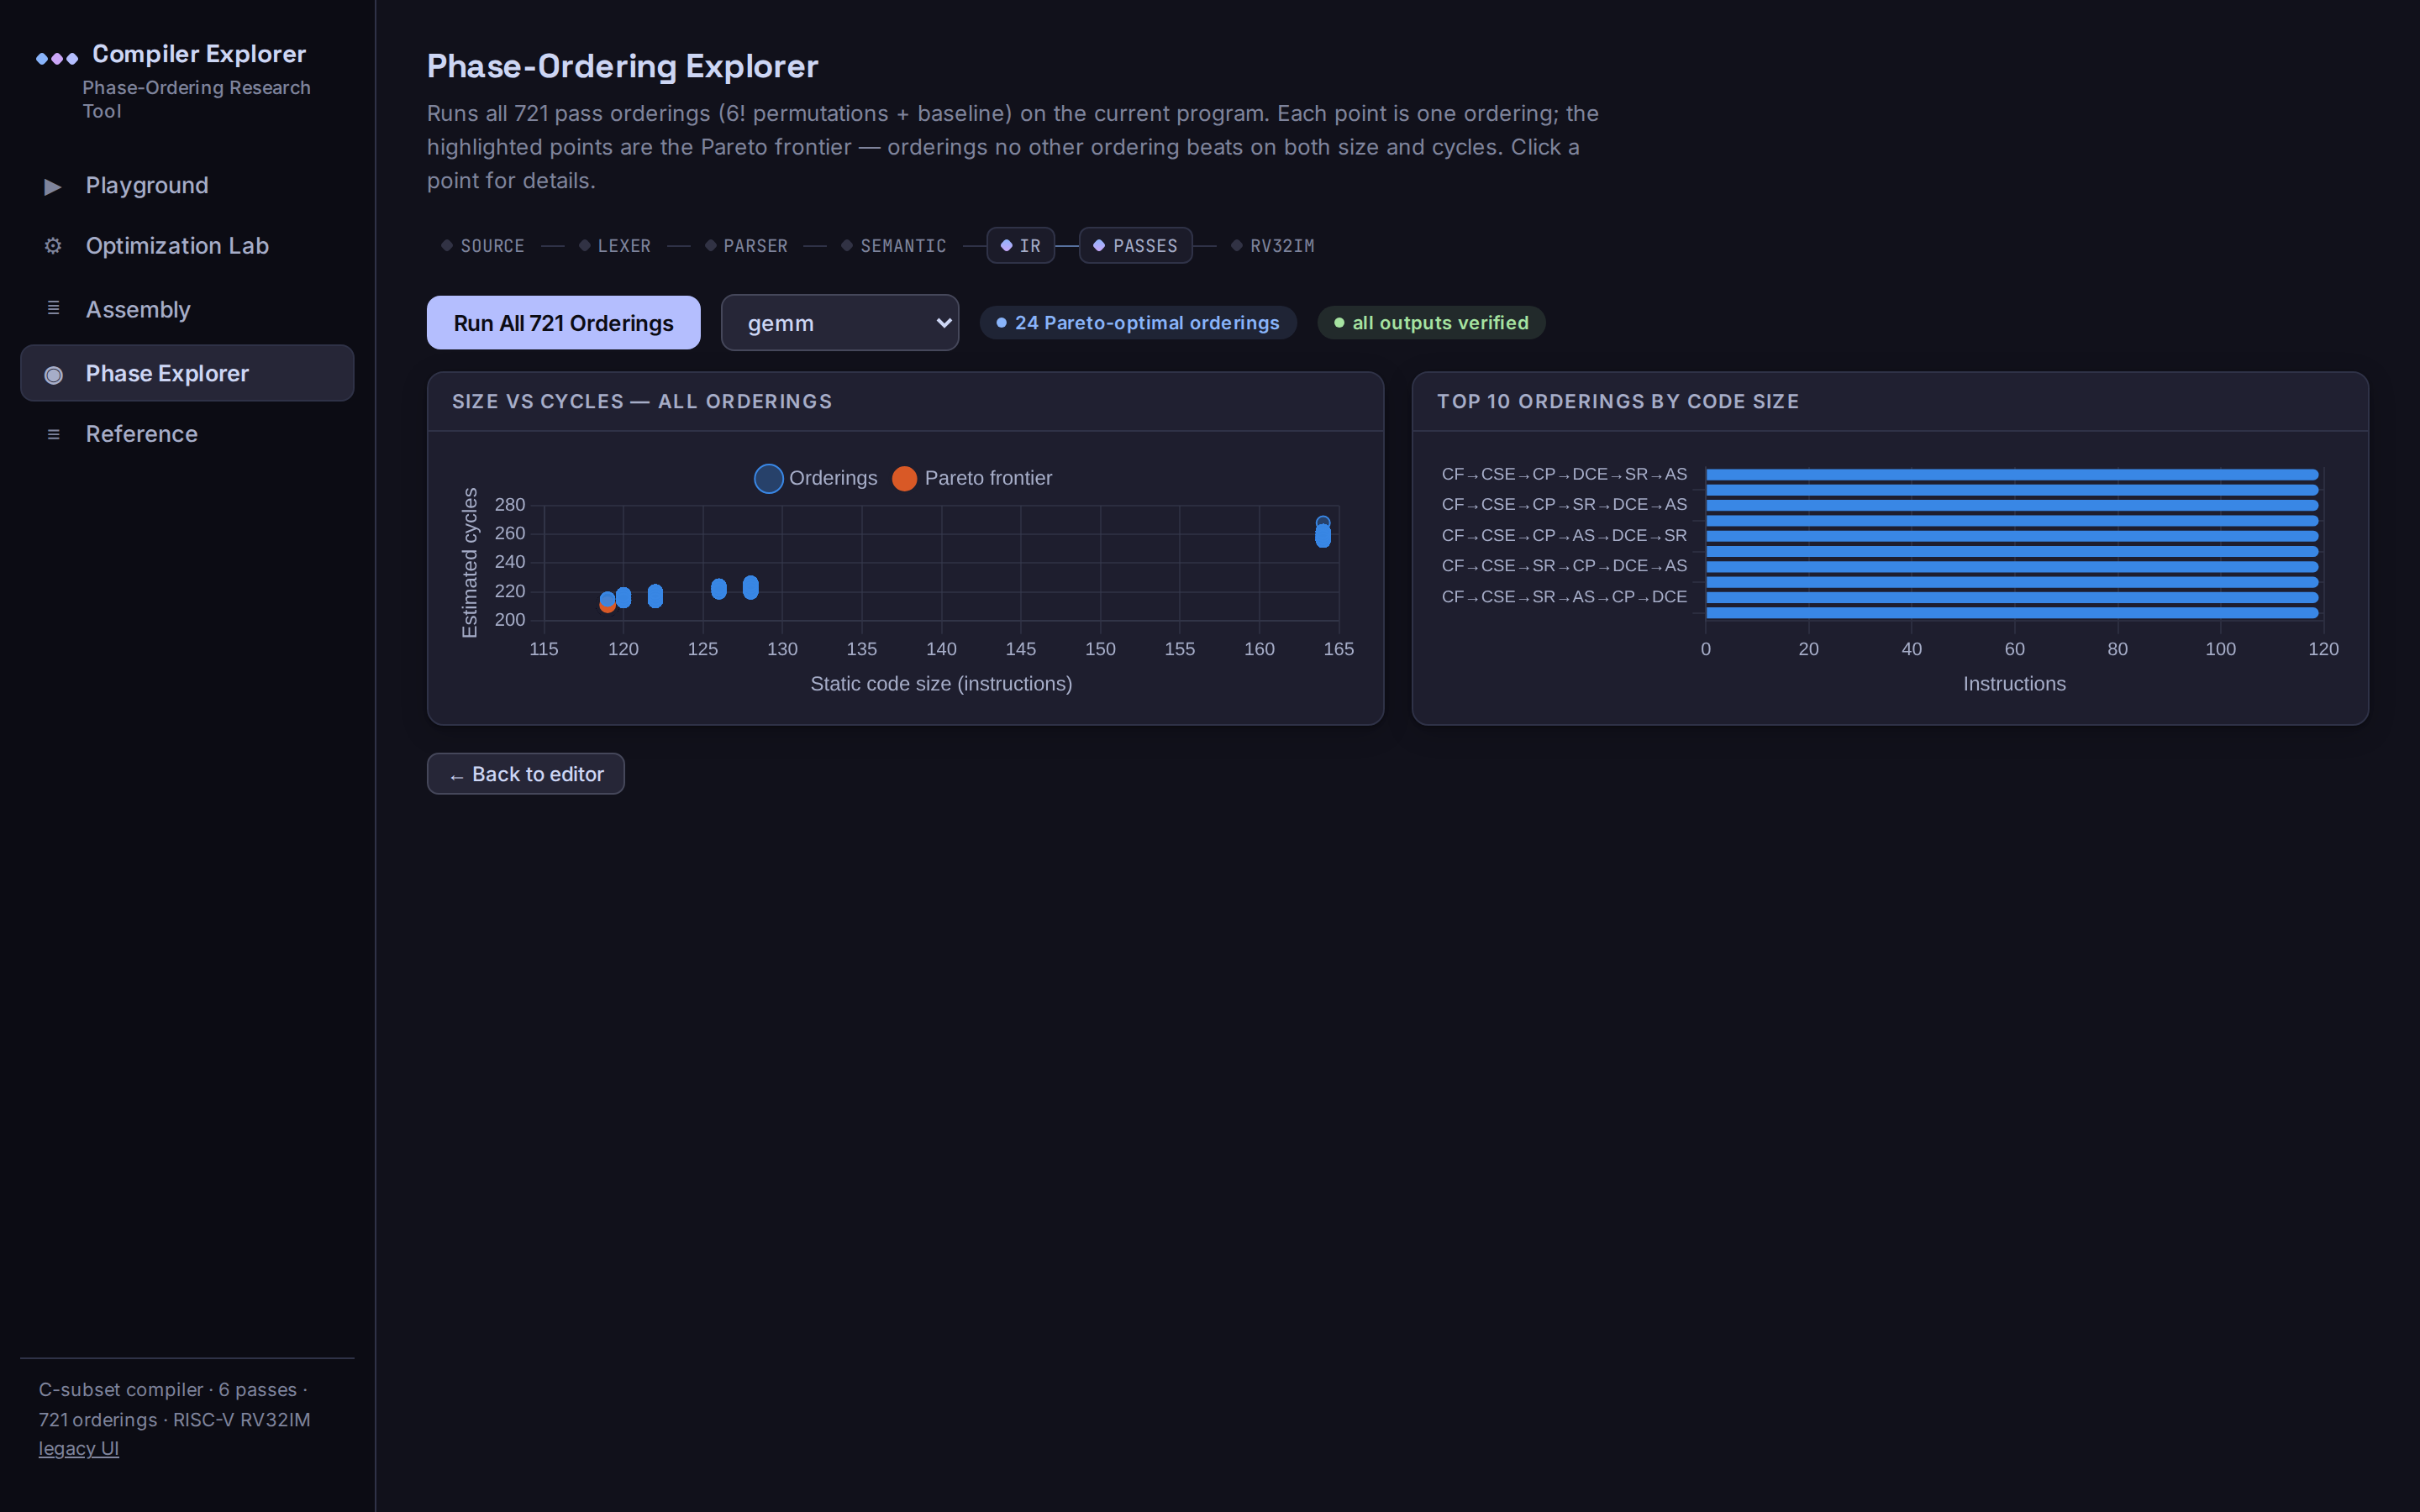
\includegraphics[width=0.82\textwidth]{gui_explorer}
\caption[Phase-Ordering Explorer page after running all 721 orderings on \code{gemm}.]{Phase-Ordering Explorer page after running all 721 orderings on \code{gemm}: size against cycles with the Pareto frontier highlighted, and the ten smallest orderings.}
\label{fig:gui-explorer}
\end{figure}

\section{Societal Impact of the Project}

The most immediate impact of the project is educational. Compiler construction is taught in every computer science programme, and optimization is the part of the course that students find most abstract, because the effects are indirect and the tools that exhibit them are too large to read. The web application turns the phase-ordering problem into something a student can manipulate in a browser within minutes: load a program, drag a pass, watch the code change. Because the whole compiler is about four thousand lines of readable Python, it also serves as a reference implementation that a student can study end to end, modify, and extend as a course project; the exhaustive results in this chapter give an instructor ground truth against which student-written passes or student-chosen orderings can be checked. The tool requires no installation beyond Python and runs offline, so it is usable in institutions with limited computing infrastructure.

The second impact is on the practice of embedded software development. India's manufacturing sector, and in particular its micro, small, and medium enterprises, increasingly builds products around low-cost microcontrollers, and the RISC-V instruction set targeted by this project's back end is becoming a common choice for such devices because it carries no licensing cost. On these devices code size determines whether a product can use a cheaper part with less flash, and executed instructions determine battery life. The study shows that on embedded-style kernels the difference between a good and a poor pass ordering is a factor of two or more in code-size reduction and a quarter of all executed instructions. A firmware team that understands this can evaluate its toolchain's options with a small effort, and the infrastructure provides a template for how such an evaluation, exhaustive, output-validated, and reported with geometric means, should be done. The longer-term prospect, identified in the future work, is an automatic ordering selector that a small manufacturer could apply without compiler expertise.

The third impact is on research practice. The project demonstrates that a complete, reproducible phase-ordering study can be carried out by an undergraduate team with a purpose-built infrastructure, and that the central phenomena reported for production compilers reproduce exactly at small scale. The repository, the benchmark suite, the results, and the tool are available for other students and researchers to build on, and the API makes the infrastructure usable as an environment for testing search and learning methods against exhaustive ground truth. Finally, the project has a modest environmental dimension: every instruction that a compiler removes from a program is energy that the program will not consume, on every device and every execution for the life of the product, and a better understanding of how to remove instructions is a small contribution to more efficient computing.

\section{SDG Mapped}

The project's objectives and outcomes align with the following United Nations Sustainable Development Goals.

\begin{itemize}
  \item \textbf{SDG 4: Quality Education.} The interactive application and the readable compiler are teaching instruments for one of the harder topics in the computer science curriculum. They are free, run offline on modest hardware, and are documented for self-study, which supports equitable access to technical education.
  \item \textbf{SDG 9: Industry, Innovation, and Infrastructure.} The project contributes tools and evidence for building more efficient embedded software on open hardware, and demonstrates a reproducible methodology for compiler evaluation that small engineering organizations can adopt. Its use of the open RISC-V architecture supports indigenous, license-free technology development.
  \item \textbf{SDG 8: Decent Work and Economic Growth.} By showing how compiler configuration affects the cost of embedded products, and by pointing towards automatic tuning that requires no compiler specialist, the project supports the productivity of micro, small, and medium enterprises that build electronic products.
  \item \textbf{SDG 7: Affordable and Clean Energy, and SDG 12: Responsible Consumption and Production (indirect).} Smaller and faster firmware consumes less energy and allows products to use smaller parts. The project quantifies one lever, pass ordering, for achieving both, and its future work targets measured energy directly.
  \item \textbf{SDG 17: Partnerships for the Goals.} The infrastructure is built on and gives back to open-source foundations, uses community benchmark suites, and is designed as a shared platform on which other institutions can run experiments and courses.
\end{itemize}

\chapter{Conclusion}

This project set out to answer a question that every compiler textbook raises and none settles quantitatively: how much does the order of optimization passes matter, and why? The answer was pursued by construction. Rather than probing a production compiler from the outside, the team built a complete compiler infrastructure for a subset of C in which six classical optimizations, constant folding, dead code elimination, common subexpression elimination, copy propagation, strength reduction, and algebraic simplification, are independent, reorderable, and individually correct passes over a three-address-code intermediate representation. Because the pass set is small, the ordering space of 720 permutations could be enumerated in full, and because the compiler is small, every result could be inspected by hand.

The empirical findings are clear. Across fifteen kernels adapted from the MiBench embedded suite and the PolyBench/C numerical suite, the best family of orderings reduces static code size by a geometric mean of 35.7\%, with per-program reductions from 22.3\% to 60.0\%, and reduces the estimated cycle cost by 20.5\% and the dynamic instruction count by 23.2\%. The worst family reduces code size by only 1.3\% and leaves thirteen of the fifteen programs entirely unchanged. Between these extremes lie only nine distinct aggregate outcomes, because the 720 orderings collapse into equivalence classes determined solely by the relative order of four passes: constant folding, copy propagation, common subexpression elimination, and dead code elimination. Strength reduction and algebraic simplification never change the instruction count and affect the cycle estimate only through their position relative to constant folding. The governing rule is simple and was confirmed on every program: the passes that expose opportunities, constant folding and copy propagation, must run before the pass that consumes them, dead code elimination, and dead code elimination should run last. Every one of the 10{,}815 optimized programs produced output identical to its baseline, and every benchmark lowered to RISC-V RV32IM assembly produced the same output in the simulator as in the interpreter, with the code-size improvement measured on the intermediate representation carried through to the assembly.

The engineering findings are equally definite. A compiler infrastructure of about four thousand lines of Python, with a hand-written lexer, a recursive-descent parser, a semantic analyzer, a linear intermediate representation with explicit def-use information, an interpreter, and a stack-slot RISC-V back end, is sufficient to conduct a complete phase-ordering study and is small enough for a student to read in full. The decision to keep every pass local to a basic block and to route all memory access through dedicated opcodes made the passes correct under arbitrary reordering without alias analysis, at a cost in optimization power that the study quantifies. The decision to validate every ordering by execution, and every lowering by simulation, caught three real bugs during development, in common subexpression elimination, in algebraic simplification, and in the interaction heatmap, that static reasoning had missed.

The interactive web application makes the study repeatable by anyone with a browser. A user can load any benchmark or write a new program, inspect every front-end artefact, drag the six passes into any order, watch the intermediate code change stage by stage with a diff and metric deltas, read the RISC-V assembly side by side with the intermediate code that produced it, and run the full exploration to see the Pareto front of size against cycles for their own code. The phase-ordering problem, which is usually described in a paragraph and then set aside, becomes something a learner can manipulate.

The results also situate the project within the literature. The observation that most orderings are redundant is the same observation that made the exhaustive enumerations of Kulkarni and colleagues feasible and that motivates the dormant-pass and dependence-modelling techniques of recent work. The rule that enabling passes must precede clean-up passes is the rule Muchnick stated from experience three decades ago, here given quantitative form on a small pass set. The strong but imperfect correlation between code size and estimated cycles across orderings mirrors the multi-objective framing of POSET-RL and COLE. The project does not claim to improve on any of these; it claims to make their central phenomena exact, visible, and teachable.

\section*{Future Scope}

The infrastructure was designed so that each of the following extensions requires adding to it rather than restructuring it.

\begin{itemize}
  \item \textbf{Global data-flow analysis.} The passes reset their state at every label. Building a control-flow graph and implementing iterative data-flow analysis for reaching definitions, live variables, and available expressions would let the same six passes work across basic blocks, and would raise a new phase-ordering question: whether the structural rules found here survive when the passes become global.
  \item \textbf{More passes and higher-order interactions.} Loop-invariant code motion, induction-variable strength reduction, function inlining, and a peephole pass over the assembly would extend the pass set to ten or more, at which point exhaustive enumeration becomes impractical and the infrastructure can serve as a test bed for the search and learning methods surveyed in Chapter 2, with the exhaustive six-pass results as ground truth.
  \item \textbf{Combined passes.} Following Click and Cooper, merging constant folding, copy propagation, and dead code elimination into a single sparse conditional constant propagation pass would test how much of the best ordering's benefit can be captured by one pass, dissolving part of the ordering problem rather than solving it.
  \item \textbf{Measured rather than estimated cost.} Running the generated assembly under a cycle-accurate simulator, or on a RISC-V development board with a cycle counter, would replace the static cost model with measurements and would allow energy to be studied directly.
  \item \textbf{Register allocation.} A linear-scan or graph-colouring allocator in the back end would remove most of the loads and stores in the generated assembly and would make the assembly-level effect of each ordering more pronounced.
  \item \textbf{Larger and real benchmarks.} Supporting more of C, in particular pointers, structures, and multi-dimensional arrays, would allow unmodified MiBench and PolyBench sources to be compiled, removing the adaptation step.
  \item \textbf{Automated ordering selection.} The equivalence-class structure found here suggests a cheap heuristic: compute the program's instruction-category profile, predict which class it falls in, and choose a representative ordering. Training such a predictor on many programs, and comparing it with the reinforcement-learning approaches in the literature, is a natural next research project.
  \item \textbf{Classroom deployment and evaluation.} The web application should be used in a compiler design course and its effect on students' understanding of pass interactions measured, in the manner of the VisOpt study.
\end{itemize}

With these extensions, the infrastructure can grow from a complete study of six passes into a general platform for phase-ordering research and teaching, while retaining the property that made this study possible: every component is small enough to read, and every result is small enough to check.


% ---------------------------------------------------------------------------
%  BACK MATTER
% ---------------------------------------------------------------------------
\clearpage
\pagestyle{backmatter}
\markboth{References}{}
\phantomsection
\addcontentsline{toc}{chapter}{References}
\begin{spacing}{1.15}
\begin{thebibliography}{99}
\setlength{\itemsep}{4pt}

\bibitem{aho2006} A. V. Aho, M. S. Lam, R. Sethi, and J. D. Ullman, \emph{Compilers: Principles, Techniques, and Tools}, 2nd ed. Boston, MA, USA: Pearson Addison-Wesley, 2006.

\bibitem{cooper2011} K. D. Cooper and L. Torczon, \emph{Engineering a Compiler}, 2nd ed. Burlington, MA, USA: Morgan Kaufmann, 2011.

\bibitem{muchnick1997} S. S. Muchnick, \emph{Advanced Compiler Design and Implementation}. San Francisco, CA, USA: Morgan Kaufmann, 1997.

\bibitem{touati2006} S.-A.-A. Touati and D. Barthou, ``On the decidability of phase ordering problem in optimizing compilation,'' in \emph{Proc. 3rd ACM Conference on Computing Frontiers (CF '06)}, Ischia, Italy, 2006, pp. 147--156.

\bibitem{lattner2004} C. Lattner and V. Adve, ``LLVM: A compilation framework for lifelong program analysis and transformation,'' in \emph{Proc. International Symposium on Code Generation and Optimization (CGO '04)}, Palo Alto, CA, USA, 2004, pp. 75--86.

\bibitem{guthaus2001} M. R. Guthaus, J. S. Ringenberg, D. Ernst, T. M. Austin, T. Mudge, and R. B. Brown, ``MiBench: A free, commercially representative embedded benchmark suite,'' in \emph{Proc. 4th IEEE International Workshop on Workload Characterization (WWC-4)}, Austin, TX, USA, 2001, pp. 3--14.

\bibitem{pouchet2016} L.-N. Pouchet and T. Yuki, ``PolyBench/C 4.2: The polyhedral benchmark suite,'' 2016. [Online]. Available: \url{https://sourceforge.net/projects/polybench/}

\bibitem{godbolt2019} M. Godbolt, ``Optimizations in C++ compilers: A practical journey,'' \emph{ACM Queue}, vol. 17, no. 5, pp. 69--100, 2019.

\bibitem{koitz2025} R. Koitz-Hristov, F. Mandl, and F. Wotawa, ``VisOpt: Visualization of compiler optimizations for computer science education,'' in \emph{Proc. 56th ACM Technical Symposium on Computer Science Education (SIGCSE TS 2025)}, Pittsburgh, PA, USA, 2025.

\bibitem{cooper1999} K. D. Cooper, P. J. Schielke, and D. Subramanian, ``Optimizing for reduced code space using genetic algorithms,'' in \emph{Proc. ACM SIGPLAN Workshop on Languages, Compilers, and Tools for Embedded Systems (LCTES '99)}, Atlanta, GA, USA, 1999, pp. 1--9.

\bibitem{almagor2004} L. Almagor, K. D. Cooper, A. Grosul, T. J. Harvey, S. W. Reeves, D. Subramanian, L. Torczon, and T. Waterman, ``Finding effective compilation sequences,'' in \emph{Proc. ACM SIGPLAN/SIGBED Conference on Languages, Compilers, and Tools for Embedded Systems (LCTES '04)}, Washington, DC, USA, 2004, pp. 231--239.

\bibitem{kulkarni2004} P. Kulkarni, S. Hines, J. Hiser, D. Whalley, J. Davidson, and D. Jones, ``Fast searches for effective optimization phase sequences,'' in \emph{Proc. ACM SIGPLAN Conference on Programming Language Design and Implementation (PLDI '04)}, Washington, DC, USA, 2004, pp. 171--182.

\bibitem{kulkarni2006} P. A. Kulkarni, D. B. Whalley, G. S. Tyson, and J. W. Davidson, ``Exhaustive optimization phase order space exploration,'' in \emph{Proc. International Symposium on Code Generation and Optimization (CGO '06)}, New York, NY, USA, 2006, pp. 306--318.

\bibitem{kulkarni2009} P. A. Kulkarni, D. B. Whalley, G. S. Tyson, and J. W. Davidson, ``Practical exhaustive optimization phase order exploration and evaluation,'' \emph{ACM Transactions on Architecture and Code Optimization}, vol. 6, no. 1, article 1, 2009.

\bibitem{ashouri2017} A. H. Ashouri, A. Bignoli, G. Palermo, C. Silvano, S. Kulkarni, and J. Cavazos, ``MiCOMP: Mitigating the compiler phase-ordering problem using optimization sub-sequences and machine learning,'' \emph{ACM Transactions on Architecture and Code Optimization}, vol. 14, no. 3, article 29, 2017.

\bibitem{hajali2020} A. Haj-Ali, Q. Huang, W. Moses, J. Xiang, I. Stoica, K. Asanovi\'{c}, and J. Wawrzynek, ``AutoPhase: Juggling HLS phase orderings in random forests with deep reinforcement learning,'' in \emph{Proc. 3rd Conference on Machine Learning and Systems (MLSys 2020)}, Austin, TX, USA, 2020.

\bibitem{jain2022} S. Jain, Y. Andaluri, S. VenkataKeerthy, and R. Upadrasta, ``POSET-RL: Phase ordering for optimizing size and execution time using reinforcement learning,'' in \emph{Proc. IEEE International Symposium on Performance Analysis of Systems and Software (ISPASS 2022)}, Singapore, 2022, pp. 121--131.

\bibitem{cummins2023} C. Cummins, V. Seeker, D. Grubisic, M. Elhoushi, Y. Liang, B. Roziere, J. Gehring, F. Gloeckle, K. Hazelwood, G. Synnaeve, and H. Leather, ``Large language models for compiler optimization,'' arXiv preprint arXiv:2309.07062, 2023.

\bibitem{georgiou2018} K. Georgiou, C. Blackmore, S. Xavier-de-Souza, and K. Eder, ``Less is more: Exploiting the standard compiler optimization levels for better performance and energy consumption,'' in \emph{Proc. 21st International Workshop on Software and Compilers for Embedded Systems (SCOPES '18)}, Sankt Goar, Germany, 2018, pp. 35--42.

\bibitem{bacon1994} D. F. Bacon, S. L. Graham, and O. J. Sharp, ``Compiler transformations for high-performance computing,'' \emph{ACM Computing Surveys}, vol. 26, no. 4, pp. 345--420, 1994.

\bibitem{whitfield1997} D. L. Whitfield and M. L. Soffa, ``An approach for exploring code improving transformations,'' \emph{ACM Transactions on Programming Languages and Systems}, vol. 19, no. 6, pp. 1053--1084, 1997.

\bibitem{click1995} C. Click and K. D. Cooper, ``Combining analyses, combining optimizations,'' \emph{ACM Transactions on Programming Languages and Systems}, vol. 17, no. 2, pp. 181--196, 1995.

\bibitem{triantafyllis2003} S. Triantafyllis, M. Vachharajani, N. Vachharajani, and D. I. August, ``Compiler optimization-space exploration,'' in \emph{Proc. International Symposium on Code Generation and Optimization (CGO '03)}, San Francisco, CA, USA, 2003, pp. 204--215.

\bibitem{hoste2008} K. Hoste and L. Eeckhout, ``Cole: Compiler optimization level exploration,'' in \emph{Proc. 6th IEEE/ACM International Symposium on Code Generation and Optimization (CGO '08)}, Boston, MA, USA, 2008, pp. 165--174.

\bibitem{agakov2006} F. Agakov, E. Bonilla, J. Cavazos, B. Franke, G. Fursin, M. F. P. O'Boyle, J. Thomson, M. Toussaint, and C. K. I. Williams, ``Using machine learning to focus iterative optimization,'' in \emph{Proc. International Symposium on Code Generation and Optimization (CGO '06)}, New York, NY, USA, 2006, pp. 295--305.

\bibitem{fursin2011} G. Fursin, Y. Kashnikov, A. W. Memon, Z. Chamski, O. Temam, M. Namolaru, E. Yom-Tov, B. Mendelson, A. Zaks, E. Courtois, F. Bodin, P. Barnard, E. Ashton, E. Bonilla, J. Thomson, C. K. I. Williams, and M. O'Boyle, ``Milepost GCC: Machine learning enabled self-tuning compiler,'' \emph{International Journal of Parallel Programming}, vol. 39, no. 3, pp. 296--327, 2011.

\bibitem{kulkarnicavazos2012} S. Kulkarni and J. Cavazos, ``Mitigating the compiler optimization phase-ordering problem using machine learning,'' in \emph{Proc. ACM International Conference on Object Oriented Programming Systems Languages and Applications (OOPSLA '12)}, Tucson, AZ, USA, 2012, pp. 147--162.

\bibitem{ashouri2018} A. H. Ashouri, W. Killian, J. Cavazos, G. Palermo, and C. Silvano, ``A survey on compiler autotuning using machine learning,'' \emph{ACM Computing Surveys}, vol. 51, no. 5, article 96, 2018.

\bibitem{cummins2022} C. Cummins, B. Wasti, J. Guo, B. Cui, J. Ansel, S. Gomez, S. Jain, J. Liu, O. Teytaud, B. Steiner, Y. Tian, and H. Leather, ``CompilerGym: Robust, performant compiler optimization environments for AI research,'' in \emph{Proc. IEEE/ACM International Symposium on Code Generation and Optimization (CGO 2022)}, Seoul, Republic of Korea, 2022, pp. 92--105.

\bibitem{venkatakeerthy2020} S. VenkataKeerthy, R. Aggarwal, S. Jain, M. S. Desarkar, R. Upadrasta, and Y. N. Srikant, ``IR2Vec: LLVM IR based scalable program embeddings,'' \emph{ACM Transactions on Architecture and Code Optimization}, vol. 17, no. 4, article 32, 2020.

\bibitem{nobre2016} R. Nobre, L. G. A. Martins, and J. M. P. Cardoso, ``A graph-based iterative compiler pass selection and phase ordering approach,'' in \emph{Proc. 17th ACM SIGPLAN/SIGBED Conference on Languages, Compilers, Tools, and Theory for Embedded Systems (LCTES 2016)}, Santa Barbara, CA, USA, 2016, pp. 21--30.

\bibitem{han2024} R. Han and H. Kim, ``Exponentially expanding the phase-ordering search space via dormant information,'' in \emph{Proc. 33rd ACM SIGPLAN International Conference on Compiler Construction (CC 2024)}, Edinburgh, UK, 2024.

\bibitem{liu2024} J. Liu et al., ``Efficient compiler optimization by modeling passes dependence,'' \emph{CCF Transactions on High Performance Computing}, 2024.

\bibitem{chen2025} Y. Chen, H. Chen, Y. Yao, P. Yu, F. Xu, and X. Ma, ``Exploiting booster pass chain for compiler phase ordering,'' \emph{ACM Transactions on Embedded Computing Systems}, 2025.

\bibitem{fleming1986} P. J. Fleming and J. J. Wallace, ``How not to lie with statistics: The correct way to summarize benchmark results,'' \emph{Communications of the ACM}, vol. 29, no. 3, pp. 218--221, 1986.

\bibitem{waterman2019} A. Waterman and K. Asanovi\'{c}, Eds., \emph{The RISC-V Instruction Set Manual, Volume I: Unprivileged ISA}, Document Version 20191213. RISC-V Foundation, 2019.

\bibitem{arm2010} ARM Limited, \emph{Cortex-M3 Technical Reference Manual}, Revision r2p1, 2010.

\bibitem{nystrom2021} R. Nystrom, \emph{Crafting Interpreters}. Genever Benning, 2021.

\bibitem{sandler2024} N. Sandler, \emph{Writing a C Compiler: Build a Real Programming Language from Scratch}. San Francisco, CA, USA: No Starch Press, 2024.

\end{thebibliography}
\end{spacing}


\appendix
\renewcommand{\chaptermark}[1]{\markboth{Appendix \thechapter}{}}
\chapter{Grammar of the Source Language}
\lstset{basicstyle=\ttfamily\scriptsize}

The grammar below is the one implemented by the recursive-descent parser, written in an informal EBNF. Terminals are in quotation marks or upper case; braces denote repetition and square brackets denote optional parts.

\begin{lstlisting}[numbers=none, caption={EBNF grammar of the C subset}, label={lst:grammar}]
program         = { global_decl | function_decl } ;
global_decl     = "int" IDENT [ "=" [ "-" ] NUMBER ] ";" ;
function_decl   = "int" IDENT "(" [ param_list ] ")" block ;
param_list      = "int" IDENT { "," "int" IDENT } ;
block           = "{" { statement } "}" ;
statement       = var_decl | array_decl | if_stmt | while_stmt | for_stmt
                | return_stmt | print_stmt | block | assign_or_expr_stmt ;
var_decl        = "int" IDENT [ "=" expr ] ";" ;
array_decl      = "int" IDENT "[" NUMBER "]" ";" ;
if_stmt         = "if" "(" expr ")" block [ "else" ( block | if_stmt ) ] ;
while_stmt      = "while" "(" expr ")" block ;
for_stmt        = "for" "(" [ var_decl | simple_stmt ";" ] [ expr ] ";"
                  [ simple_stmt ] ")" block ;
return_stmt     = "return" [ expr ] ";" ;
print_stmt      = "print" "(" expr ")" ";" ;
assign_or_expr_stmt = simple_stmt ";" ;
simple_stmt     = expr [ "=" expr ] ;
                  (* assignment target must be IDENT or IDENT "[" expr "]" *)
expr            = or_expr ;
or_expr         = and_expr { "||" and_expr } ;
and_expr        = equality { "&&" equality } ;
equality        = comparison { ( "==" | "!=" ) comparison } ;
comparison      = addition { ( "<" | ">" | "<=" | ">=" ) addition } ;
addition        = multiplication { ( "+" | "-" ) multiplication } ;
multiplication  = unary { ( "*" | "/" | "%" ) unary } ;
unary           = ( "-" | "!" ) unary | primary ;
primary         = NUMBER
                | IDENT [ "(" [ expr { "," expr } ] ")" | "[" expr "]" ]
                | "(" expr ")" ;
\end{lstlisting}

Tokens: \code{NUMBER} is a non-empty sequence of decimal digits not immediately followed by a letter or underscore; \code{IDENT} is a letter or underscore followed by letters, digits, or underscores, excluding the seven keywords \code{int}, \code{if}, \code{else}, \code{while}, \code{for}, \code{return}, and \code{print}. Whitespace and both comment forms (\code{//} to end of line and \code{/* ... */}) are ignored between tokens.

\chapter{Intermediate Representation Opcode Reference}

Table~\ref{tab:opcode-ref} lists every opcode with its printed form, the variable it defines, the variables it uses, and its cost in the cycle model. Operands written in lower case are variable, temporary, or label names; \code{k} is an integer literal. Instructions marked ``side effect'' are never removed by dead code elimination.

\begin{table}[!ht]
\centering\scriptsize\renewcommand{\arraystretch}{1.0}
\caption{Complete opcode reference}
\label{tab:opcode-ref}
\begin{tabular}{L{2.6cm} L{3.6cm} L{1.2cm} L{1.4cm} C{1.3cm} L{3.4cm}}
\toprule
\textbf{Opcode} & \textbf{Printed form} & \textbf{Defines} & \textbf{Uses} & \textbf{Cost} & \textbf{Notes}\\
\midrule
ADD, SUB, MUL, DIV, MOD & \code{d = a op b} & d & a, b & 1, 1, 3, 12, 12 & DIV, MOD by 0 give 0\\
NEG & \code{d = -a} & d & a & 1 & \\
EQ, NEQ, LT, GT, LTE, GTE & \code{d = a cmp b} & d & a, b & 1 & result 0 or 1\\
AND, OR & \code{d = a \&\& b}, \code{d = a || b} & d & a, b & 1 & eager; result 0 or 1\\
NOT & \code{d = !a} & d & a & 1 & \\
COPY & \code{d = a} & d & a & 1 & \\
LOAD\_CONST & \code{d = k} & d & -- & 1 & \\
LABEL & \code{L:} & -- & -- & 0 & structural; resets pass state\\
JUMP & \code{goto L} & -- & -- & 2 & side effect\\
JUMP\_IF\_TRUE & \code{if a goto L} & -- & a & 2 & side effect\\
JUMP\_IF\_FALSE & \code{iffalse a goto L} & -- & a & 2 & side effect\\
PARAM & \code{param a} & -- & a & 1 & side effect; queued for CALL\\
CALL & \code{d = call f, n} & d & -- & 5 & side effect; resets pass state\\
RETURN & \code{return [a]} & -- & a & 3 & side effect\\
FUNC\_BEGIN & \code{func f:} & -- & -- & 0 & structural\\
FUNC\_END & \code{end func f} & -- & -- & 0 & structural\\
FUNC\_PARAM & \code{param\_decl p} & -- & -- & 0 & binds argument to p\\
PRINT & \code{print a} & -- & a & 10 & side effect; output oracle\\
ARR\_DECL & \code{arr a[k]} & -- & -- & 0 & zero-initialized\\
ARR\_LOAD & \code{d = a[i]} & d & i & 2 & never cached by CSE\\
ARR\_STORE & \code{a[i] = v} & -- & i, v & 2 & side effect\\
GLOBAL\_DECL & \code{global g = k} & -- & -- & 0 & .data in back end\\
GLOBAL\_LOAD & \code{d = @g} & d & -- & 2 & \\
GLOBAL\_STORE & \code{@g = a} & -- & a & 2 & side effect\\
NOP & \code{nop} & -- & -- & 0 & from folded jumps; not printed\\
\bottomrule
\end{tabular}
\end{table}

\chapter{Complete Compilation Trace of the factorial Benchmark}

This appendix shows every artefact the compiler produces for the \code{factorial} benchmark under the best ordering, so that the numbers reported in Chapter 5 can be checked by hand.

\begin{lstlisting}[language=CSubset, caption={Source of the factorial benchmark}, label={lst:factorial-src}]
int factorial(int n) {
    int result = 1;
    int i = 1;
    while (i <= n) {
        result = result * i;
        i = i + 1;
    }
    return result;
}

int main() {
    /* Constant expressions that can be folded */
    int base = 2 + 3;
    int extra = 10 - 5;

    int val = factorial(base);
    print(val);

    /* Dead code: result never used */
    int unused = 42 * 2;
    int also_unused = unused + 100;

    /* Common subexpression: base + extra computed twice */
    int sum1 = base + extra;
    int sum2 = base + extra;
    print(sum1);
    print(sum2);

    return 0;
}
\end{lstlisting}

\begin{lstlisting}[language=ThreeAC, caption={Unoptimized three-address code: 40 instructions counted for code size, 81 estimated cycles, 81 instructions executed. Output: 120, 10, 10.}, label={lst:factorial-base}]
func factorial:
  param_decl n
  t0 = 1
  result = t0
  t1 = 1
  i = t1
L0:
  t2 = i <= n
  iffalse t2 goto L1
  t3 = result * i
  result = t3
  t4 = 1
  t5 = i + t4
  i = t5
  goto L0
L1:
  return result
end func factorial
func main:
  t6 = 2
  t7 = 3
  t8 = t6 + t7
  base = t8
  t9 = 10
  t10 = 5
  t11 = t9 - t10
  extra = t11
  param base
  t12 = call factorial, 1
  val = t12
  print val
  t13 = 42
  t14 = 2
  t15 = t13 * t14
  unused = t15
  t16 = 100
  t17 = unused + t16
  also_unused = t17
  t18 = base + extra
  sum1 = t18
  t19 = base + extra
  sum2 = t19
  print sum1
  print sum2
  t20 = 0
  return t20
end func main
\end{lstlisting}

\begin{lstlisting}[language=ThreeAC, caption={After CF, CSE, CP, DCE, SR, AS: 16 instructions, 55 estimated cycles, 53 instructions executed. Output: 120, 10, 10 (identical).}, label={lst:factorial-opt}]
func factorial:
  param_decl n
  result = 1
  i = 1
L0:
  t2 = i <= n
  iffalse t2 goto L1
  t3 = result * i
  result = t3
  t5 = i + 1
  i = t5
  goto L0
L1:
  return result
end func factorial
func main:
  param 5
  t12 = call factorial, 1
  print t12
  print 10
  print 10
  return 0
end func main
\end{lstlisting}

Note that the loop body of \code{factorial} is not shortened: \code{result = t3} and \code{i = t5} survive because \code{result} and \code{i} are redefined on every iteration, so the single-assignment condition for constant propagation does not hold and the copies cannot be propagated across the loop label. This is the cost of block-local analysis, discussed in Chapter 5.

The RV32IM assembly generated from the optimized program is 59 instructions long against 119 for the unoptimized program; it can be viewed with \code{python -m compiler.main compiler/benchmarks/programs/factorial.c -O CF,CSE,CP,DCE,SR,AS --emit-asm} or on the Assembly page of the web application (\fig{fig:gui-assembly}).

\chapter{Test Suite Summary}

The test suite is run with \code{python -m pytest}; all 185 test cases pass in about four seconds on the reference machine. Tables~\ref{tab:tests} and~\ref{tab:tests2} summarize the suite by test class.

\begin{table}[H]
\centering\scriptsize\renewcommand{\arraystretch}{1.0}
\caption{Automated test suite by module and class: compiler core}
\label{tab:tests}
\begin{tabular}{L{2.4cm} L{5.0cm} C{0.9cm} L{5.0cm}}
\toprule
\textbf{Module} & \textbf{Test class} & \textbf{Cases} & \textbf{What is verified}\\
\midrule
\code{test\_compiler.py}
 & TestLexer & 12 & tokens, comments, positions, lexical errors\\
 & TestParser & 11 & every statement form, precedence, parse errors\\
 & TestSymbolTable & 5 & scopes, shadowing, duplicates\\
 & TestIRGenerator & 8 & lowering of each construct, IR formatting\\
 & TestConstantFolding & 3 & folding, propagation, non-folding of variables\\
 & TestDeadCodeElimination & 3 & dead assignments, unreachable code, liveness\\
 & TestCommonSubexpression\-Elimination & 4 & reuse, invalidation on redefinition\\
 & TestPassManager & 5 & orderings, validation, description\\
 & TestVisualizer & 3 & interaction matrix, plot de-duplication\\
 & TestMetrics & 6 & code size, cycles, array costs, breakdown\\
 & TestEndToEnd & 3 & all orderings valid; optimization never grows code\\
 & TestCopyPropagation, TestStrength\-Reduction, TestAlgebraic\-Simplification & 19 & each rewrite rule; unsound rules absent\\
 & TestInterpreter & 9 & arithmetic, loops, calls, recursion, dynamic count\\
 & TestCrossPassIntegration, TestArrays & 12 & all benchmarks under all orderings; array pipeline\\
\bottomrule
\end{tabular}
\end{table}

\begin{table}[H]
\centering\scriptsize\renewcommand{\arraystretch}{1.0}
\caption{Automated test suite by module and class (continued): language features, back end, and web API}
\label{tab:tests2}
\begin{tabular}{L{2.4cm} L{5.0cm} C{0.9cm} L{5.0cm}}
\toprule
\textbf{Module} & \textbf{Test class} & \textbf{Cases} & \textbf{What is verified}\\
\midrule
\code{test\_new\_features.py}
 & TestSemanticAnalyzer & 14 & every semantic rule; all benchmarks pass analysis\\
 & TestElseIf, TestForLoop & 7 & parsing and execution; orderings preserve output\\
 & TestShortCircuit & 4 & right operand skipped; 0/1 normalization\\
 & TestGlobals & 7 & cross-function state; DCE never removes stores\\
 & TestRiscvBackend & 9 & structure, exit code, printing, division by zero, recursion, arrays, globals; all benchmarks match interpreter in the simulator\\
 & TestErrorHierarchy & 2 & all phase errors share one base class\\
\midrule
\code{test\_web.py}
 & TestCompileEndpoint, TestOptimizeEndpoint & 7 & success and structured error responses\\
 & TestExamplesEndpoint & 7 & listing, suite classification, doc extraction, path traversal rejected\\
 & TestBenchmarkEndpoint, TestIndexPage & 4 & 721 results; React and legacy pages served\\
 & TestSemanticPhase, TestAssemblyField & 6 & semantic errors via API; assembly and mapping endpoints\\
\bottomrule
\end{tabular}
\end{table}


\end{document}
